% !TEX encoding = UTF-8 Unicode
% preamble for the RiTeh thesis template

\documentclass[botnum,a4paper,11,oneside,final]{tex_aux/rithesis}
%\usepackage[latin1]{inputenc}
%\usepackage[T1]{fontenc}
%\usepackage[english]{babel}
%%%%%%% adjustment for croatian
\usepackage[croatian]{babel}
\usepackage[cp1250]{inputenc}	% this ensures croatian special letters are correctly printed with Windows

\usepackage{graphicx}	% this enables import of graphics
\usepackage[labelsep=space,format=hang]{caption}  % adjusts caption style
\usepackage{subfig}	% this enables use of subfigures
\usepackage{amsmath}
\usepackage{amssymb}
%\usepackage{fancyhdr}
\usepackage{amsfonts}
%\usepackage{amsthm}
%\usepackage{pdfsync}
% This package is used to tell TeXShop where things are in the PDF file.
% Command-click at any spot in the PDF and it will jump to the corresponding
% location in the source file.
\usepackage{epsfig}		% to use eps figures; maybe not necessary to use here with Mac
\usepackage{epstopdf}	% this automatically converts any eps-figure into a pdf-figure
\usepackage[section]{placeins} % da slika ne upada u sljedeci section

\hyphenation{sko-ko-vi-toj}

\DeclareGraphicsRule{.tif}{png}{.png}{`convert #1 `dirname #1`/`basename #1 .tif`.png}	% this converts any tif-figure into a png-figure (Mac directly supports pdf, jpg, png, and mps formats, but additionally can use tif and eps when they are automatically converted in png, and pdf, respectively, using the above two packages
\DeclareGraphicsExtensions{.pdf,.jpeg,.jpg,.png}  % ekstenzije koje ne treba pisati uz ime slike
\graphicspath{{slike/}}   % mjesto gdje su smjestene slike

%\usepackage{makeidx}	% this enables creation of index
%\usepackage{showidx}
%\makeindex			% this makes index automatically, based on author's entries

%\usepackage{eufrak}
%\usepackage[mathcal]{euscript}
\usepackage{psfrag}
%\usepackage{url} 
\usepackage{hyperref}
\hypersetup{
breaklinks,
colorlinks=true,
linkcolor=black,
citecolor=black,
filecolor=black,
urlcolor=black
}

\setcounter{topnumber}{1} \setcounter{bottomnumber}{1}

\newcommand{\navod}[1]{``#1''}


\begin{document}

\frontmatter   % - ne dirati

% upisati naziv studija
\degreesubject{Diplomski studij ra\v{c}unarstva} % upisati odgovarajuci naziv studija

% upisati vrstu rada
\documenttype{Diplomski rad}  % Zavrsni rad ili Diplomski rad

\title{Ispitivanje Near Field Communication i Bluetooth Low Energy tehnologija na Android ure\dj ajima}   % upisati specificni naslov rada

\date{Svibanj, \thisyear.}   % upisati samo aktualni mjesec predaje rada

\author{Dino Biki\'{c}}  % upisati svoje ime i prezime
\jmbag{0069053128}  % upisati vlastiti JMBAG
\maketitle		% ne dirati

%\makecopyright

% Okruzenje za pisanje posvete. Maknuti komentare ukoliko se želi napisati posvetu.
%\begin{dedication}
	%Ovo je posveta nekome
%\end{dedication}

% Okruzenje za pisanje zahvale
%\begin{acknowledgments} % maknuti komentare ukoliko se želi napisati zahvalu
	%\include{Zahvala}  
	% tekst upisati u datoteku ``Zahvala'' i ukloniti komentar ili ga upisati izravno ovdje
%\end{acknowledgments}

\mentor{Miroslav Joler}   % zamijeniti podacima o svojem mentoru
\maketitleabstract

% kreira mjesto za umetnuti stranicu s opisom zadatka - ne dirati
\begin{assignmentpage}
\end{assignmentpage}

% kreira mjesto za umetnuti stranicu s izjavom o samostalnoj izradbi zadatka - ne dirati
\begin{honestystatementpage}
\end{honestystatementpage}

% kreiranje popisa sadrzaja, slika i tabela - ništa ne dirati
\tableofcontents
\listoffigures


% Lista kratica koristenih u tekstu. Kratice upisati u datoteku ``Kratice.tex'' koja je prilozena u paketu.
% Nije obavezno. Ako se ne zeli koristiti, onda ovaj blok staviti u komentar pomocu znaka %
\begin{glossary}{Longest string}
	% ovo je primjer koristenja, a student neka to zamijeni svojim kraticama i doda sve koje zeli
% ako se ne zeli deklarirati popis kratica, onda ga staviti pod komentar u glavnoj datoteci

   \item[{\bf 3DES}]	Triple Data Encryption Algorithm
   \item[{\bf AES}]	Advanced Encryption Standard
   \item[{\bf API}]	Application Program Interface
   \item[{\bf ART}]	Android Runtime
   \item[{\bf ASK}]	Amplitude-Shift Keying
   \item[{\bf BLE}]	Bluetooth Low Energy
   \item[{\bf BLP}]	Blood Pressure Profile 
   \item[{\bf CMS}]	Content Management System
   \item[{\bf CSCP}]	Cycling Speed and Cadence Profile
   \item[{\bf CSS}]	Cascading Style Sheets
   \item[{\bf ESN}]	Electronic Serial Number
   \item[{\bf FAB}]	Floating Action Button
   \item[{\bf FeliCa}]	Felicity Card
   \item[{\bf FMP}]	Find Me Profile
   \item[{\bf GAP}]	Generic Access Profile
   \item[{\bf GATT}]	Generic Attribute Profile 
   \item[{\bf GFSK}]	Gaussian Frequency Shift Modulation
   \item[{\bf GSM}]	Global System for Mobile Communications
   \item[{\bf GLP}]	Glucose Profile
   \item[{\bf HID }]	Human Interface Device
   \item[{\bf HOGP }]	HID over GATT Profile
   \item[{\bf HRP }]	Heart Rate Profile 
   \item[{\bf HTML }]	Hypertext Markup Language
   \item[{\bf HTTP }]	Hypertext Transfer Protocol
   \item[{\bf IMEI }]	International Mobile Station Equipment Identity
   \item[{\bf JSON }]	JavaScript Object Notation
   \item[{\bf MEID}]	Mobile Equipment Identifier
   \item[{\bf MVP}]	Model View Presenter
   \item[{\bf NDEF}]	NFC Data Exchange Format
   \item[{\bf NFC}]	Near Field Communication
   \item[{\bf PHP}]	Hypertetxt Preprocessor
   \item[{\bf POI}]	Point of Interes
   \item[{\bf PXP}]	Proximity Profile
   \item[{\bf RFID}]	Radio-Frequency Identification
   \item[{\bf SDK}]	Software Developtment Kit 
   \item[{\bf SFTP}]	Secure File Transfer Protocol
   \item[{\bf SIG}]	Bluetooth Special Interest Group
   \item[{\bf SQL}]	Structured Querry Language
   \item[{\bf URI}]	Uniform Resource Identifier
   \item[{\bf XML}]	Extensible Markup Language
   \item[{\bf VM}]	Virtual Machine
\end{glossary}

% kreiranje glavnoga dijela rada
\mainmatter		% ne dirati


% Ovdje pomoæu include funkcije ucitavati kreirana poglavlja. Poglavljima dajte logicna imena s obzirom na sadrzaj prikazan u njima (bez razmaka u imenu).

%\chapter{Kako koristiti paket za pisanje Zavr�noga rada u \LaTeX-u}
Ovo su uvodne napomene za kori�tenje predlo�ka za pisanje Zavr�noga ili Diplomskoga rada studenata Tehni�koga fakulteta u Rijeci.

Paket je pripremljen tako da student �to prije mo�e pisati vlastiti tekst u ve� pripremljenom predlo�ku koji �e, uz minimalno u�enje sintakse \LaTeX-a, studentu olak�ati urediti svoj rad. U paketu su uklju�ene potrebne upute i sintakti�ke strukture koje bi trebale udovoljiti potrebama ve�ine studenta, a dodatne informacije postoje u priru�nicima odnosno na web stranicama na internetu koje su posve�ene \LaTeX-u (vidi u nastavku).

{\color{red} POZOR: paket treba biti prekopiran negdje na disk ne mijenjaju�i originalnu strukturi mapa (foldera) i ne mijenjaju�i nazive datoteka koje su u mapi \emph{tex\_aux}!}

\section{Opis sadr�aja paketa}
Paket se sastoji od
\begin{itemize}
 \item datoteke \href{UPUTE.pdf}{\emph{UPUTE.pdf}} koja sadr�i postupak instalacije potrebnih alata na ra�unalo te kori�tenja paketa. \emph{UPUTE} su bazirane na Windows OS, a korisnici drugih OS si na nazna�enim web lokacijama samo trebaju na�i instalacije za njihov OS.
 \item \verb|JMBAG_Ime_Prezime.tex| datoteke koja je sredi�nja datoteka koja povezuje sve cjeline i kompajliranjem koje se dobije izlazni \verb|JMBAG_Ime_Prezime.pdf| dokument.\\ U ovoj se datoteci inicijalno nalaze i upute za kori�tenje paketa kao i primjeri osnovne uporabe naj�e��ih sintakti�kih struktura u \LaTeX-u koje bi trebale biti dovoljne ve�ini studenata za pisanje rada.
 %
 \item \verb|tex_aux| mape u kojoj su interne datoteke koje definiraju stilove i dr. Student s njima ne treba \emph{ni�ta} raditi, ali one trebaju biti u \verb|tex_aux| mapi pod glavnom mapom Zavr�noga rada, kao �to je postavljeno u ovom paketu
 %
 \item mape \emph{slike} u koju student treba pohraniti sve slike koje �e koristiti u radu. Ime mape se ne smije preimenovati bez boljega poznavanja sintakse \LaTeX-a jer ovaj paket da bi ispravno radio o�ekuje ba� takvo ime mape
 %
 \item datoteke \verb|sintaksa_cestih_struktura.tex| koja ne sudjeluje izravno u kompajliranju pdf dokumenta, nego slu�i kao repozitorij u kojem su sadr�ane naj�e��e potrebne sintakti�ke strukture koje su spremne za kopiranje uz minimalnu prilagodbu parametara u studentovu radu
 %
 \item mape \href{run:manuals}{{\color{blue}manuals}} u kojoj se nalazi nekoliko najpopularnijih priru�nika za uporabu \LaTeX-a. 
\end{itemize}
%%%%%%%%%%%%%%%%%%%%%%%%%%%%%%%%%%%%%%%%%%%%%%%%%%%%%%%%%%%%%%%

\section{�ime se opremiti za pisanje rada}
Da bi se rad napisao pomo�u \LaTeX-a (a vrijedi svake lipe!), najprije je na ra�unalo potrebno instalirati (barem) \LaTeX~ software, a uz to, premda nije nu�an za pisanje rada, preporu�am i \emph{JabRef} software koji pomo�u intuitivnih su�elja korisniku omogu�ava kreiranje popisa literature na vrlo sofisticirani na�in. 

\subsection{Instalacija \LaTeX-a}
\begin{enumerate}
	\item odite na sredi�nji \LaTeX~ portal: \url{http://www.latex-project.org/}
	\item kliknite na poveznicu \href{http://www.latex-project.org/ftp.html}{Getting LaTeX} i potom uo�ite i povucite instalaciju koja odgovara va�em OSu (npr.\ proTeXt za Windows, MacTeX za Mac, TeX Live za Linux). Pozor: download je velik i mo�e du�e potrajati �ak i na brzoj vezi---dajte si dovoljno vremena za obaviti download.
	\item Instalirajte \LaTeX~ nabavljen u prethodnoj to�ki slijede�i upute koje su date za tu instalaciju (npr. proTeXt za Windowse daje kratki pdf s uputama koje vas vode kroz instalaciju korak po korak).
	\item Instalirajte si tekst-editor koji je pogodan za pisanje \LaTeX~ koda (npr.\ za Windows je popularan TeXnicCenter i dolazi ve� upakiran u proTeXt-u, za Mac je kvalitetan TeXShop koji sada tako�er dolazi u paketu s MacTeX-om).
\end{enumerate}

\subsection{Instalacija \emph{JabRef} softvera}
\emph{JabRef} je legalno besplatno dostupni softver za Windows OS (za druge OS �ete isto na�i takve programe) koji nam omogu�ava opisivanje literature na lak na�in pomo�u intuitivnih su�elja, a kao rezultat kreira \emph{BibTeX} datoteku \emph{ime.bib} (gdje je \emph{ime} koje korisnik proizvoljno dodijeli pri pohrani) u kojoj je literatura opisana na na�in koji \LaTeX~ razumije i na osnovi toga automatski formira popis literature na kraju na�ega rada, a sukladno redoslijedu pozivanja pojedine literature u tekstu.

\emph{Napomena: Kori�tenje BiBTeX programa kakav je \emph{JabRef} nije neophodno, ali prakti�no je. Alternativni---lo�iji---na�in jest ru�no opisati kori�tenu literaturu unutar \emph{tex} datoteke.\\ U datoteci po imenu \href{run:Literatura.tex}{{\color{blue}Literatura.tex}} koja je uklju�ena u ovaj paket ve� su namje�tene postavke kao da �e se literatura opisati pomo�u BiBTeX programa (npr.\ JabRef) i ne treba ni�ta mijenjati, a ispod toga se mo�e pro�itati upute i za drugi na�in (p)opisivanja literature.}

Instalacijska datoteka za \emph{JabRef} se mo�e prona�i na webu na adresi \url{http://jabref.sourceforge.net/}.
Preporu�eni postupak:
\begin{enumerate}
	\item povucite si i instalirajte posljednju stabilnu verziju \emph{JabRef}-a
	\item inicijalno se upoznajte s najva�nijim opcijama u \emph{JabRef}-u:
	\begin{enumerate}
		\item uo�ite ikonu (pod znakom ``+'' i tekstom \emph{New BibTeX Entry}) za unos nove jedinice literature (npr. knjige, �lanka, web portala i sl.)
		\item kada kliknete za unos nove stavke literature, uo�ite kakvi se sve tipovi literature nude za odabir. Odabirom opcije koja odgovara naslovu koji �elite unijeti, otvorit �e vam se novi prozor s poljima u koja se mo�e unijeti informacije o literaturi. Za odabrani tip literature samo su neka polja obavezna (nalaze se pod karticom (eng.\ \emph{tabom}) \emph{Required fields}), dok se pod drugim karticama mo�e i ne mora unijeti dodatne informacije.
		\item prije nego pohranite va� unos sa \emph{Ctrl+S}, morate toj jedinici dodijeliti jedinstveni identifikator, tzv.\ \emph{Bibtexkey}, �to je jedno od polja koja su obavezna za unos. Mo�ete ru�no upisati neki proizvoljni string, ali pogodnije je generirati ga automatski. Za to u�initi me�u ikonama na vrhu imate ikonu koja izgleda kao (�arobni) �tapi� sa zvjezdicama oko njega, klikom na kojega \emph{JabRef} automatski dodijeli jedinstveni BibTeX \emph{klju�} za tu bibliografsku jedinicu. Pomo�u toga klju�a se poslije bilo kada i bilo gdje u pisanju va�ega rada mo�ete pozvati na tu referencu, a \LaTeX~ �e sve ostalo obaviti za vas tj.\ dodijeliti joj odgovaraju�i broj u tekstu i s tim brojem uvrstiti u popis literature.
		\item korisnik ima mogu�nost i promijeniti uzorak po kojem se kreira struktura automatski generiranoga jedinstvenoga BibTeX klju�a tako da se ode u opciju izbornika \emph{Options $>>$ Preferences $>>$ BibTeX key generator} gdje je na vrhu prozora prikazan \emph{default} uzorak, npr. \verb|[auth]:[year]| �to zna�i da se klju� kreira na bazi \verb|prezime(autora):godina(rada)|. To se sada mo�e urediti po nekom novom uzorku, no ovako definirani uzorak u biti zadovoljava, a ako igdje ima potrebe za dodatnim razlikovanjem, mo�e se automatski generiran klju� jo� ru�no napraviti korekcija dodavanjem na kraju npr.\ \verb|_a| itd.
		\item klikom na karticu \emph{BibTeX source} mo�ete vidjeti kako �e unos va�ih podataka zapravo biti zapisan u va�oj \emph{ime.bib} datoteci koja �e se formirati od svih bibliografskih jedinica koje unesete.
		\item Za \emph{ime} va�e bibliografske datoteke kod pohrane odaberite \emph{Literatura} jer to ime o�ekuje ovaj paket. Ina�e se mo�e dodijeliti proizvoljno ime, ali onda treba znati �to i gdje promijeniti u sredi�njoj \LaTeX~ datoteci. Pozor: Datoteka \emph{Literatura.bib} koju ste tako kreirali mora se nalaziti unutar mape ovoga paketa da bi sve ispravno radilo! U paketu je za primjer ve� kreirana jedna datoteka istoga imena koju za vje�bu student mo�e i otvoriti u \emph{JabRef}-u, ali to su samo pokazne bibliografske jedinice unesene kao primjer, koje student treba u kona�nici zamijeniti svojim stvarnim podacima.
	\end{enumerate}
\end{enumerate} 
%%%%%%%%%%%%%%%%%%%%%%%%%%%%%%%%%%%%%%%%%%%%%%%%%%%

\section{Kako (kona�no) po�eti pisati svoj rad}
Najbr�i start je sljede�i:
\begin{enumerate}
	\item Pokrenite va� \LaTeX~tekst-editor i iz njega otvorite pripremljeni predlo�ak za pisanje rada \href{run:JMBAG_Ime_Prezime.tex}{{\color{blue}JMBAG\_Ime\_Prezime.tex}} koji se nalazi unutar ovoga paketa (obi�no ga se mo�e otvoriti i dvostrukim klikom na \emph{tex} datoteku ukoliko �e OS koristiti \LaTeX~ editor za otvaranje iste)
	\item skrolajte niz dokumentu ni�ta ne mijenjaju�i, dok ne nai�ete na retke u kojima su kratke upute koje upu�uju studenta �to treba upisati u pripremljenu naredbu. U biti, u gornjem dijelu dokumenta nema u biti ni�ega za mijenjati, nego tek nakon linije koja sadr�i \verb|\begin{document}|. Specifi�ni podaci koje student treba upisati bit �e uz naredbe:
	%
		\begin{itemize}
			\item \verb|\degreesubject|: upisati vrstu studija (preddiplomski ili diplomski studij studentovoga usmjerenja)
			\item \verb|\documenttype|: upisati \emph{Zavr�ni rad} ili \emph{Diplomski rad}
			\item \verb|\title|: upisati naslov rada
			\item \verb|\date|: upisati samo mjesec predaje rada. Godina se upisuje automatski.
			\item \verb|\author|: upisati ime i prezime studenta
			\item \verb|\jmbag|: zamijeniti postoje�i broj vlastitim JMBAG brojem 
			\item \verb|\mentor|: upisati titulu i ime i prezime svojega mentora
		\end{itemize}
	%
	\item Za prvu probu nakon une�enih podataka, kompajlirajte dokument na na�in da unutar va�ega tekst-editora odaberete opciju izbornika (odnosno ikonu) koja glasi ne�to poput \emph{Build and View (Current File)}. To pokrene postupak kompajliranja svega i rezultat bi trebao biti \emph{pdf} datoteka u kojoj �ete vidjeti lijepo formatirane po�etne stranice rada. Pozor: 
		\begin{itemize}
			\item provjerite u postavkama editora da je izlazni format PDF. To se ili vidi negdje na ekranu va�ega editora ili negdje pod opcijom koja glasi poput \emph{Select Output Profile} (vjerojatno pod \emph{Build} izbornikom) i nudi par izlaznih formata jedan od kojih je PDF.
			\item nekada je potrebno 2-3 puta pokrenuti \emph{Build} operaciju da bi sve promjene bile a�urirane u \emph{pdf} dokumentu kao �to su npr.\ brojevi referenca, popis literature i sl.
		\end{itemize}
		%
	\item Za (i vi�e nego) osnovnu sintaksu mo�ete otvoriti datoteku \href{run:Intro.tex}{{\color{blue}Intro.tex}} koja je dio paketa i unutar koje su napisane i ove upute. Vidjet �ete da da se odmah mo�e pisati va� tekst uz nekoliko osnovnih naredaba, kao �to su:
	\begin{itemize}
		\item \verb|\chapter{Naslov poglavlja}| kojim definirate naslov poglavlja
		\item \verb|\section{Naslov sekcije}| kojim definirate naslov sekcije unutar poglavlja
		\item \verb|\subsection{Naslov podsekcije}| kojim definirate naslov podsekcije
		\item \verb|\cite{bibtexkey}| kojom se pozivate na odre�enu literaturu jedinstveni klju� koje je u BibTeX datoteci \href{run:Literatura.bib}{{\color{blue}Literatura.bib}} dan sa \emph{bibtex key}
		\item \verb|\emph{tekst}| naredbu kojom se pomo�u italic slova nagla�ava neka rije� ili fraza
		\item \verb|\href| ili \verb|\url| naredba kojom se kreira poveznica na neku URL adresu ili dokument (ne pretjerujte s tim, odnosno uop�e ne morate to koristiti u radu, nego za vanjske reference koristiti samo \verb|\cite{}| naredbu, a za unutra�nje reference (na dijelove teksta) kombinaciju naredbi \verb|\label{ID}| i \verb|\ref{ID}| gdje se prvu postavi na dio teksta na koji �emo se poslije referencirati, a drugu na mjestu s kojega se referenciramo)
		\item ostale sintakse kao �to su ubacivanje slike, tabele ili jednad�ba mo�ete na�i u datoteci \href{run:sintaksa_cestih_struktura.tex}{{\color{blue}sintaksa\_cestih\_struktura.tex}} koja je dio paketa. Odabrane se strukture mo�e kopirati i zalijepiti u va� tekst, uz minimalne prilagodbe kao �to su naziv slike, veli�ina slike, opis i ID slike, a analogno i za tabele i jednad�be.
		\item Kona�no, za vi�e detalja o bilo �emu, potra�ite informacije u priru�nicima koji su prilo�eni u mapi \href{run:manuals}{{\color{blue}manuals}} ili na webu, gdje se, me�u obiljem drugih informacija, nalaze i korisne \href{http://en.wikibooks.org/wiki/LaTeX/}{wiki stranice} o \LaTeX-u pomo�u kojih se obi�no brzo prona�e upute i zadovoljavaju�e rje�enje kojom sintaksom se mo�e urediti �eljeni dio teksta.
  	\end{itemize}
\item Savjet: svako poglavlje napi�ite u novoj datoteci koju imenujte prikladnim imenom (bez razmaka u imenu) i potom ih samo pozivajte iz glavnoga dokumenta \emph{JMBAG\_Ime\_Prezime.tex} pomo�u \verb|\include{ime_datoteke}| naredbe.
\end{enumerate}

Nadam se da �e vam ovaj dokument pomo�i u pripremi teksta va�ega rada i omogu�iti tro�iti glavninu vremena na sadr�aj rada, a manje na formatiranje rada jer to bi za vas sada trebao obaviti \LaTeX! 
No, fair-playa radi, potrebno je napomenuti i sljede�e: \LaTeX~ je vrlo osjetljiv na pogre�ke u sintaksi naredbi (da, ba� kao svaki programski jezik) pa vas mo�e povremeno zagnjaviti javljanjem pogre�ke koju nikako ne uspijevate uo�iti gdje je. Iskustvo kojim se izbjegava ta nelagoda jest sljede�e:
\begin{itemize}
	\item budite koncentrirani dok pi�ete \LaTeX~naredbe
	\item kompajlirajte tekst prije nego se skupi puno teksta jer tako �ete imati manje teksta za prekontrolirati u slu�aju pogre�ke
	\item ako niste sigurni ho�e li vam raditi neka naredba nakon pisanja, radije odmah kompajlirajte tekst da vidite �to �ete dobiti i rije�ite dvojbu, nego �ekati da se skupi jo� dubioza, kada �e biti te�e detektirati koja naredba zapravo izaziva probleme (\LaTeX~ov prozor s porukama nije odve� precizan u lociranju i opisu pogre�aka)
\end{itemize}

%%%%%%%% POGLAVLJE ZAVRSENO %%%%%%%%%%%%%%%


\chapter{Primjeri naj�e��ih sintakti�kih struktura}
Ovo se poglavlje u ovome trenutku i ne mora �itati, ali za one koje se �ele bolje pripremiti prije samoga po�etka pisanja rada, sigurno �e pomo�i. 

U nastavku su opisane naj�e��e sintakti�ke strukture, a koje za budu�e potrebe imate pohranjene i u datoteci \href{run:sintaksa_cestih_struktura.tex}{{\color{blue}sintaksa\_cestih\_struktura.tex}} koja je sastavni dio glavne mape ovoga paketa.

\section{Ubacivanje slike}
Na Slici~\ref{fig:prva} je prikazana osnovna shema HPM sustava.
\begin{figure}[!htbp]
	\begin{center}
 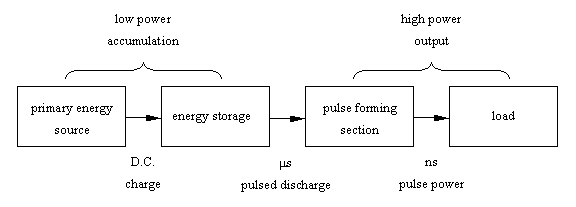
\includegraphics[height=4cm,width=8cm,keepaspectratio=true]{HPMsystem}
 \caption{Primjer ubacivanja slike}
 \label{fig:prva}
	\end{center}
\end{figure}

Znak \verb|~| iza rije�i Slici osigurava to�no jedan znak razmaka, �to poma�e ukoliko je rij�e Slika na kraju retka, da ne razdvoji rije� Slika i pripadaju�i broj slike.
Parametri slike \emph{width} i \emph{height} odre�uju maksimalne dopu�tene dimenzije pri �emu se primarno po�tuje manju navedenu dimenziju, a \emph{keepaspectratio} osigurava zadr�avanje odnosa dimenzija slike, odnosno sprje�ava deformaciju slike, nakon proizvoljno unesenih veli�ina.

Uo�i da sve oznake tj.\ \emph{labeli} ne smiju imati razmak u imenu. To vrijedi i op�enito, a ne samo za slike.

Tako�er, uo�i da nije potrebno pisati ekstenziju slike jer to je ure�eno u postavkama glavnoga dokumenta pa time �tedi trud. Ekstenzije koje se mo�e izostaviti su: \emph{jpg}, \emph{jpeg}, \emph{png} i \emph{pdf}.

Shema prikazana na Slici~\ref{fig:prva} �e biti kori�tena i za potrebe idu�ih primjera, a {\color{blue} u mapi na va�em disku ju obri�ite nakon �to po�nete pohranjivati vlastite slike vezane uz va� rad}.


\section{Ubacivanje podslika}
%
\begin{figure}[!htpb]
	  \begin{center}
	   \subfloat[kra�i opis podslike a]{\label{fig:HPM_a} 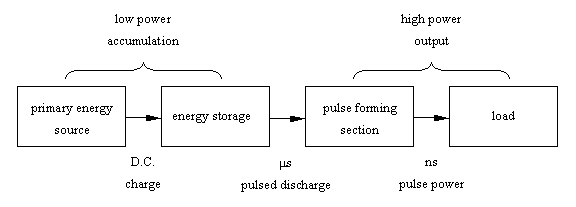
\includegraphics[height=5cm,width=8cm,keepaspectratio=true]{HPMsystem}} \\ %\hspace{10pt}
	   \subfloat[kra�i opis podslike b]{\label{fig:HPM_b} 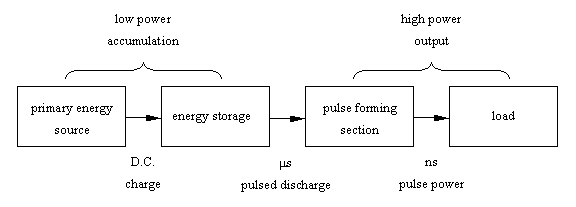
\includegraphics[height=5cm,width=8cm,keepaspectratio=true]{HPMsystem}}
\caption{Primjer ubacivanja vi�e podslika. Ovo je opis cijele slike.}
\label{fig:HPMsystem_2}
	  \end{center}
\end{figure}

Na Slici~\ref{fig:HPMsystem_2} su prikazane dvije podslike. 
Podslika~\ref{fig:HPM_a} pokazuje shemu HPM sustava, a podslika~\ref{fig:HPM_b} -- to isto.


\section{Ubacivanje tabele} \label{tabela}
Vi�e detalja o kreiranju tabela pro�itajte u literaturi, a sljede�i blok vam omogu�ava kreiranje jednostavne tabele, kao �to je prikazano u Tabeli~\ref{tab:prva}.
\begin{table}[!htbp]
\caption{Ovo je primjer izrade tabele}
\centering
\begin{tabular}{|c|c|c|}
\hline
variabla & vrijednost 1 & vrijednost 2  \\ [0.5ex]
\hline \hline  
A & 5 & 3 \\ [0.5ex]
B & 4 & 2 \\ [0.5ex]
\hline
\end{tabular}
\label{tab:prva}
\end{table}

Podaci koji su u stupcima se u tabeli razdvajaju znakom \&. Novi redak se na kraju aktualnoga retka formira znakom \verb|\\|. Broj stupaca se definira iza \emph{tabular} time �to se navedu slova koja ozna�avaju poravnavanje teksta u svakom stupcu, a broj slova zna�i broj stupaca koji �e biti kreiran u tabeli.


\section{Referenca na literaturu, sekciju, stranicu}
Na pojedinu se literaturu jednostavno uputi kori�tenjem naredbe \verb|\cite{bitex_key}| gdje je \emph{bibtex\_key} identifikator te bibliografske jedinice u bibtex datoteci. Npr.\ \verb|\cite{latex}| �e u tekstu pokazati broj te bibliografske jedinice u uglatoj zagradi \cite{latex}, te ju s istim brojem uvrsiti u popis literature (Bibliografiju) na kraju rada.

Ako se �elimo referirati na tekst u nekoj drugoj sekciji, kao npr. na dio gdje se opisuje kreiranje tabele, tada kraj te sekcije stavimo oznaku \verb|\label{ID}|, npr.\ \verb|\label{tabela}|, a na �eljenom mjestu u tekstu se na to referiramo pomo�u \verb|\ref{ID}|, npr.\ \verb|\ref{tabela}|. Tako mo�emo onda napisati da je kreiranje tabele opisano u Sekciji~\verb|~\ref{tabela}|, �to proizvede tekst koji glasi ``u Sekciji~\ref{tabela}''.

Ako �elimo navesti stranicu u na�em radu u kojoj se nalazi neki dio informacije o kojem govorimo, tada na isti na�in primijenimo \verb|\label{ID}| oznaku, a za referiranje na tu stranicu koristimo sintaksu \verb|\pageref{ID}|. 
Tako npr.\ mo�emo re�i da je primjer kreiranja tabele opisan na stranici~\verb|\pageref{tabela}|, �to �e za rezultat ima tekst u kojem pi�e da je primjer kreiranja tabele ``opisan na stranici~\pageref{tabela}''.

\section{Nagla�avanje teksta}
\subsection{Navodnici}
Za navodnike s lijeve strane fraze (otvaranje navodnika) koristi se 2x jednostruki navodnik koji se na tipkovnici nalazi lijevo od broja 1, a za navodnike s desne strane fraze (zatvaranja navodnika) se koristi 2x jednostruki navodnik koji se na tipkovnici nalazi na tipki \emph{�}, �to proizvede npr.\ ``abc''.

Alternativno, u ovom paketu je pripremljena i naredba \verb|\navod{abc}| gdje je \emph{abc} tekst koji se stavlja izme�u navodnika, tj.\ \navod{abc}.

\subsection{Kosa i podebljana slova}
Nagla�eni tekst (sli�no kosim slovima) mo�emo dobiti uporabom naredbe \verb|\emph{abc}| gdje je \emph{abc} neki tekst koji se �eli naglasiti.

Kosa slova (italic) mo�emo dobiti uporabom naredbe \verb|\textit{abc}| gdje je \textit{abc} neki tekst koji se �eli naglasiti.

Podebljana slova mo�emo posti�i uporabom naredbe \verb|\textbf{abc}| gdje je \textbf{abc} neki tekst koji �elimo podebljati.

\section{Verbatim okru�enje}
Verbatim okru�enje omogu�ava ispis teksta u izvornom obliku, bez da ga \LaTeX~ tuma�i po svojoj default sintaksi. To je pogodno kada se npr.\ na stranicu �eli kopirati dio programskoga koda iz nekog jezika i �elimo zadr�ati sve izvorne znakove, a ne da \LaTeX po�ne javljati pogre�ke kod kompajliranja jer �e ih bez toga interpretirati kao pogre�ke u sintaksi.

Postoji kra�i i du�i oblik verbatima. Kra�i slu�i za kra�u frazu od jedne ili par rije�i, a du�i za vi�e redaka.

Kra�i ima sintaksu: \verb+\verb|neka fraza|+

Du�i ima sintaksu:\\
\verb|\begin{verbatim}| \\
\verb|neki tekst| \\
\verb|\end{verbatim}| \\


\section{Kreiranje jedne jednad�be ili serije jednad�ba}

\subsection{Kreiranje jedne jednad�be}
Jednad�ba se napi�e u posebnom matemati�kom modu koji se kreira pomo�u bloka:
\begin{equation}
 A = B + C   \label{eq:prva}
\end{equation}

Jednad�ba~\eqref{eq:prva} je jedna jednostavna numerirana jednad�ba. Ako ju se ne �eli numerirati, onda se nakon rije�i \emph{begin} stavi zvjezdica, tj.\ \emph{begin\*}.

\subsection{Kreiranje vi�e jednad�ba}
Vi�e se jednad�ba kreira \emph{subequations} blokom:
\begin{subequations}
Dvije jednad�be mogu npr.\ glasiti:
\begin{align}
        A &= B + C  				\label{subeq:prva} \\
        D &= F + G				  \label{subeq:druga}
\end{align}
\label{subeq:obje}
\end{subequations}

U \eqref{subeq:prva} je prikazano dobivanje vrijednosti $A$, a u \eqref{subeq:druga} je prikazano dobivanje vrijednosti $D$. Jed.~\eqref{subeq:obje} je �uveni studentov zakon!

\section{Liste}
Liste su �este forme u tekstu kojima se na pregledni na�in nabrajaju neke stavke. Stavke obi�no navodimo s to�kama na po�etku, ili s brojevima ili sa slovima. U \LaTeX~u su upravo ta tri stila unaprijed definirana, a mogu�e su i slo�enije definicije stilova i kombinacije lista.

\subsection{Lista s to�kama}
Lista s to�kama se postigne blokom
\begin{verbatim}
\begin{itemize}
	\item prva stavka
	\item druga stavka
\end{itemize}
\end{verbatim}
�to na ekranu proizvede:
\begin{itemize}
	\item prva stavka
	\item druga stavka
\end{itemize}

\subsection{Numerirana lista s brojevima}
Numerirana lista s brojevima se postigne blokom
\begin{verbatim}
\begin{enumerate}
	\item prva stavka
	\item druga stavka
\end{enumerate}
\end{verbatim}
�to na ekranu proizvede:
\begin{enumerate}
	\item prva stavka
	\item druga stavka
\end{enumerate}


\subsection{Slov�ano numerirana lista}
Takva se lista mo�e posti�i u sklopu op�enitije forme koja omogu�uje proizvoljni opis ispred pojedine stavke, pomo�u sljede�ega bloka:
\begin{verbatim}
\begin{description}
	\item[a)] prva stavka
	\item[b)] druga stavka
\end{description}
\end{verbatim}
�to na ekranu proizvede:
\begin{description}
	\item[a)] prva stavka
	\item[b)] druga stavka
\end{description}



\section{Zavr�ne napomene}
Ovime zaklju�ujemo upute koje �e najve�em broju studenata biti dovoljne (ili barem dovoljna osnova) za uspje�no pisanje Zavr�noga odnosno Diplomskoga rada.

Prije nego prije�ete na kreiranje vlastitoga sadr�aja u�inite sljede�e:
\begin{enumerate}
	\item u mapi \href{run:slike}{{\color{blue}slike}}, obri�ite datoteku \verb|HPMsystem.png| jer je ona samo slu�ila za ilustracije u uputama
	%
	\item u glavnoj datoteci  \href{run:JMBAG\_Ime\_Prezime.tex}{{\color{blue}JMBAG\_Ime\_Prezime.tex}} stavite znak komentare ``\%'' ispred linije \verb|\chapter{Kako koristiti paket za pisanje Zavr�noga rada u \LaTeX-u}
Ovo su uvodne napomene za kori�tenje predlo�ka za pisanje Zavr�noga ili Diplomskoga rada studenata Tehni�koga fakulteta u Rijeci.

Paket je pripremljen tako da student �to prije mo�e pisati vlastiti tekst u ve� pripremljenom predlo�ku koji �e, uz minimalno u�enje sintakse \LaTeX-a, studentu olak�ati urediti svoj rad. U paketu su uklju�ene potrebne upute i sintakti�ke strukture koje bi trebale udovoljiti potrebama ve�ine studenta, a dodatne informacije postoje u priru�nicima odnosno na web stranicama na internetu koje su posve�ene \LaTeX-u (vidi u nastavku).

{\color{red} POZOR: paket treba biti prekopiran negdje na disk ne mijenjaju�i originalnu strukturi mapa (foldera) i ne mijenjaju�i nazive datoteka koje su u mapi \emph{tex\_aux}!}

\section{Opis sadr�aja paketa}
Paket se sastoji od
\begin{itemize}
 \item datoteke \href{UPUTE.pdf}{\emph{UPUTE.pdf}} koja sadr�i postupak instalacije potrebnih alata na ra�unalo te kori�tenja paketa. \emph{UPUTE} su bazirane na Windows OS, a korisnici drugih OS si na nazna�enim web lokacijama samo trebaju na�i instalacije za njihov OS.
 \item \verb|JMBAG_Ime_Prezime.tex| datoteke koja je sredi�nja datoteka koja povezuje sve cjeline i kompajliranjem koje se dobije izlazni \verb|JMBAG_Ime_Prezime.pdf| dokument.\\ U ovoj se datoteci inicijalno nalaze i upute za kori�tenje paketa kao i primjeri osnovne uporabe naj�e��ih sintakti�kih struktura u \LaTeX-u koje bi trebale biti dovoljne ve�ini studenata za pisanje rada.
 %
 \item \verb|tex_aux| mape u kojoj su interne datoteke koje definiraju stilove i dr. Student s njima ne treba \emph{ni�ta} raditi, ali one trebaju biti u \verb|tex_aux| mapi pod glavnom mapom Zavr�noga rada, kao �to je postavljeno u ovom paketu
 %
 \item mape \emph{slike} u koju student treba pohraniti sve slike koje �e koristiti u radu. Ime mape se ne smije preimenovati bez boljega poznavanja sintakse \LaTeX-a jer ovaj paket da bi ispravno radio o�ekuje ba� takvo ime mape
 %
 \item datoteke \verb|sintaksa_cestih_struktura.tex| koja ne sudjeluje izravno u kompajliranju pdf dokumenta, nego slu�i kao repozitorij u kojem su sadr�ane naj�e��e potrebne sintakti�ke strukture koje su spremne za kopiranje uz minimalnu prilagodbu parametara u studentovu radu
 %
 \item mape \href{run:manuals}{{\color{blue}manuals}} u kojoj se nalazi nekoliko najpopularnijih priru�nika za uporabu \LaTeX-a. 
\end{itemize}
%%%%%%%%%%%%%%%%%%%%%%%%%%%%%%%%%%%%%%%%%%%%%%%%%%%%%%%%%%%%%%%

\section{�ime se opremiti za pisanje rada}
Da bi se rad napisao pomo�u \LaTeX-a (a vrijedi svake lipe!), najprije je na ra�unalo potrebno instalirati (barem) \LaTeX~ software, a uz to, premda nije nu�an za pisanje rada, preporu�am i \emph{JabRef} software koji pomo�u intuitivnih su�elja korisniku omogu�ava kreiranje popisa literature na vrlo sofisticirani na�in. 

\subsection{Instalacija \LaTeX-a}
\begin{enumerate}
	\item odite na sredi�nji \LaTeX~ portal: \url{http://www.latex-project.org/}
	\item kliknite na poveznicu \href{http://www.latex-project.org/ftp.html}{Getting LaTeX} i potom uo�ite i povucite instalaciju koja odgovara va�em OSu (npr.\ proTeXt za Windows, MacTeX za Mac, TeX Live za Linux). Pozor: download je velik i mo�e du�e potrajati �ak i na brzoj vezi---dajte si dovoljno vremena za obaviti download.
	\item Instalirajte \LaTeX~ nabavljen u prethodnoj to�ki slijede�i upute koje su date za tu instalaciju (npr. proTeXt za Windowse daje kratki pdf s uputama koje vas vode kroz instalaciju korak po korak).
	\item Instalirajte si tekst-editor koji je pogodan za pisanje \LaTeX~ koda (npr.\ za Windows je popularan TeXnicCenter i dolazi ve� upakiran u proTeXt-u, za Mac je kvalitetan TeXShop koji sada tako�er dolazi u paketu s MacTeX-om).
\end{enumerate}

\subsection{Instalacija \emph{JabRef} softvera}
\emph{JabRef} je legalno besplatno dostupni softver za Windows OS (za druge OS �ete isto na�i takve programe) koji nam omogu�ava opisivanje literature na lak na�in pomo�u intuitivnih su�elja, a kao rezultat kreira \emph{BibTeX} datoteku \emph{ime.bib} (gdje je \emph{ime} koje korisnik proizvoljno dodijeli pri pohrani) u kojoj je literatura opisana na na�in koji \LaTeX~ razumije i na osnovi toga automatski formira popis literature na kraju na�ega rada, a sukladno redoslijedu pozivanja pojedine literature u tekstu.

\emph{Napomena: Kori�tenje BiBTeX programa kakav je \emph{JabRef} nije neophodno, ali prakti�no je. Alternativni---lo�iji---na�in jest ru�no opisati kori�tenu literaturu unutar \emph{tex} datoteke.\\ U datoteci po imenu \href{run:Literatura.tex}{{\color{blue}Literatura.tex}} koja je uklju�ena u ovaj paket ve� su namje�tene postavke kao da �e se literatura opisati pomo�u BiBTeX programa (npr.\ JabRef) i ne treba ni�ta mijenjati, a ispod toga se mo�e pro�itati upute i za drugi na�in (p)opisivanja literature.}

Instalacijska datoteka za \emph{JabRef} se mo�e prona�i na webu na adresi \url{http://jabref.sourceforge.net/}.
Preporu�eni postupak:
\begin{enumerate}
	\item povucite si i instalirajte posljednju stabilnu verziju \emph{JabRef}-a
	\item inicijalno se upoznajte s najva�nijim opcijama u \emph{JabRef}-u:
	\begin{enumerate}
		\item uo�ite ikonu (pod znakom ``+'' i tekstom \emph{New BibTeX Entry}) za unos nove jedinice literature (npr. knjige, �lanka, web portala i sl.)
		\item kada kliknete za unos nove stavke literature, uo�ite kakvi se sve tipovi literature nude za odabir. Odabirom opcije koja odgovara naslovu koji �elite unijeti, otvorit �e vam se novi prozor s poljima u koja se mo�e unijeti informacije o literaturi. Za odabrani tip literature samo su neka polja obavezna (nalaze se pod karticom (eng.\ \emph{tabom}) \emph{Required fields}), dok se pod drugim karticama mo�e i ne mora unijeti dodatne informacije.
		\item prije nego pohranite va� unos sa \emph{Ctrl+S}, morate toj jedinici dodijeliti jedinstveni identifikator, tzv.\ \emph{Bibtexkey}, �to je jedno od polja koja su obavezna za unos. Mo�ete ru�no upisati neki proizvoljni string, ali pogodnije je generirati ga automatski. Za to u�initi me�u ikonama na vrhu imate ikonu koja izgleda kao (�arobni) �tapi� sa zvjezdicama oko njega, klikom na kojega \emph{JabRef} automatski dodijeli jedinstveni BibTeX \emph{klju�} za tu bibliografsku jedinicu. Pomo�u toga klju�a se poslije bilo kada i bilo gdje u pisanju va�ega rada mo�ete pozvati na tu referencu, a \LaTeX~ �e sve ostalo obaviti za vas tj.\ dodijeliti joj odgovaraju�i broj u tekstu i s tim brojem uvrstiti u popis literature.
		\item korisnik ima mogu�nost i promijeniti uzorak po kojem se kreira struktura automatski generiranoga jedinstvenoga BibTeX klju�a tako da se ode u opciju izbornika \emph{Options $>>$ Preferences $>>$ BibTeX key generator} gdje je na vrhu prozora prikazan \emph{default} uzorak, npr. \verb|[auth]:[year]| �to zna�i da se klju� kreira na bazi \verb|prezime(autora):godina(rada)|. To se sada mo�e urediti po nekom novom uzorku, no ovako definirani uzorak u biti zadovoljava, a ako igdje ima potrebe za dodatnim razlikovanjem, mo�e se automatski generiran klju� jo� ru�no napraviti korekcija dodavanjem na kraju npr.\ \verb|_a| itd.
		\item klikom na karticu \emph{BibTeX source} mo�ete vidjeti kako �e unos va�ih podataka zapravo biti zapisan u va�oj \emph{ime.bib} datoteci koja �e se formirati od svih bibliografskih jedinica koje unesete.
		\item Za \emph{ime} va�e bibliografske datoteke kod pohrane odaberite \emph{Literatura} jer to ime o�ekuje ovaj paket. Ina�e se mo�e dodijeliti proizvoljno ime, ali onda treba znati �to i gdje promijeniti u sredi�njoj \LaTeX~ datoteci. Pozor: Datoteka \emph{Literatura.bib} koju ste tako kreirali mora se nalaziti unutar mape ovoga paketa da bi sve ispravno radilo! U paketu je za primjer ve� kreirana jedna datoteka istoga imena koju za vje�bu student mo�e i otvoriti u \emph{JabRef}-u, ali to su samo pokazne bibliografske jedinice unesene kao primjer, koje student treba u kona�nici zamijeniti svojim stvarnim podacima.
	\end{enumerate}
\end{enumerate} 
%%%%%%%%%%%%%%%%%%%%%%%%%%%%%%%%%%%%%%%%%%%%%%%%%%%

\section{Kako (kona�no) po�eti pisati svoj rad}
Najbr�i start je sljede�i:
\begin{enumerate}
	\item Pokrenite va� \LaTeX~tekst-editor i iz njega otvorite pripremljeni predlo�ak za pisanje rada \href{run:JMBAG_Ime_Prezime.tex}{{\color{blue}JMBAG\_Ime\_Prezime.tex}} koji se nalazi unutar ovoga paketa (obi�no ga se mo�e otvoriti i dvostrukim klikom na \emph{tex} datoteku ukoliko �e OS koristiti \LaTeX~ editor za otvaranje iste)
	\item skrolajte niz dokumentu ni�ta ne mijenjaju�i, dok ne nai�ete na retke u kojima su kratke upute koje upu�uju studenta �to treba upisati u pripremljenu naredbu. U biti, u gornjem dijelu dokumenta nema u biti ni�ega za mijenjati, nego tek nakon linije koja sadr�i \verb|\begin{document}|. Specifi�ni podaci koje student treba upisati bit �e uz naredbe:
	%
		\begin{itemize}
			\item \verb|\degreesubject|: upisati vrstu studija (preddiplomski ili diplomski studij studentovoga usmjerenja)
			\item \verb|\documenttype|: upisati \emph{Zavr�ni rad} ili \emph{Diplomski rad}
			\item \verb|\title|: upisati naslov rada
			\item \verb|\date|: upisati samo mjesec predaje rada. Godina se upisuje automatski.
			\item \verb|\author|: upisati ime i prezime studenta
			\item \verb|\jmbag|: zamijeniti postoje�i broj vlastitim JMBAG brojem 
			\item \verb|\mentor|: upisati titulu i ime i prezime svojega mentora
		\end{itemize}
	%
	\item Za prvu probu nakon une�enih podataka, kompajlirajte dokument na na�in da unutar va�ega tekst-editora odaberete opciju izbornika (odnosno ikonu) koja glasi ne�to poput \emph{Build and View (Current File)}. To pokrene postupak kompajliranja svega i rezultat bi trebao biti \emph{pdf} datoteka u kojoj �ete vidjeti lijepo formatirane po�etne stranice rada. Pozor: 
		\begin{itemize}
			\item provjerite u postavkama editora da je izlazni format PDF. To se ili vidi negdje na ekranu va�ega editora ili negdje pod opcijom koja glasi poput \emph{Select Output Profile} (vjerojatno pod \emph{Build} izbornikom) i nudi par izlaznih formata jedan od kojih je PDF.
			\item nekada je potrebno 2-3 puta pokrenuti \emph{Build} operaciju da bi sve promjene bile a�urirane u \emph{pdf} dokumentu kao �to su npr.\ brojevi referenca, popis literature i sl.
		\end{itemize}
		%
	\item Za (i vi�e nego) osnovnu sintaksu mo�ete otvoriti datoteku \href{run:Intro.tex}{{\color{blue}Intro.tex}} koja je dio paketa i unutar koje su napisane i ove upute. Vidjet �ete da da se odmah mo�e pisati va� tekst uz nekoliko osnovnih naredaba, kao �to su:
	\begin{itemize}
		\item \verb|\chapter{Naslov poglavlja}| kojim definirate naslov poglavlja
		\item \verb|\section{Naslov sekcije}| kojim definirate naslov sekcije unutar poglavlja
		\item \verb|\subsection{Naslov podsekcije}| kojim definirate naslov podsekcije
		\item \verb|\cite{bibtexkey}| kojom se pozivate na odre�enu literaturu jedinstveni klju� koje je u BibTeX datoteci \href{run:Literatura.bib}{{\color{blue}Literatura.bib}} dan sa \emph{bibtex key}
		\item \verb|\emph{tekst}| naredbu kojom se pomo�u italic slova nagla�ava neka rije� ili fraza
		\item \verb|\href| ili \verb|\url| naredba kojom se kreira poveznica na neku URL adresu ili dokument (ne pretjerujte s tim, odnosno uop�e ne morate to koristiti u radu, nego za vanjske reference koristiti samo \verb|\cite{}| naredbu, a za unutra�nje reference (na dijelove teksta) kombinaciju naredbi \verb|\label{ID}| i \verb|\ref{ID}| gdje se prvu postavi na dio teksta na koji �emo se poslije referencirati, a drugu na mjestu s kojega se referenciramo)
		\item ostale sintakse kao �to su ubacivanje slike, tabele ili jednad�ba mo�ete na�i u datoteci \href{run:sintaksa_cestih_struktura.tex}{{\color{blue}sintaksa\_cestih\_struktura.tex}} koja je dio paketa. Odabrane se strukture mo�e kopirati i zalijepiti u va� tekst, uz minimalne prilagodbe kao �to su naziv slike, veli�ina slike, opis i ID slike, a analogno i za tabele i jednad�be.
		\item Kona�no, za vi�e detalja o bilo �emu, potra�ite informacije u priru�nicima koji su prilo�eni u mapi \href{run:manuals}{{\color{blue}manuals}} ili na webu, gdje se, me�u obiljem drugih informacija, nalaze i korisne \href{http://en.wikibooks.org/wiki/LaTeX/}{wiki stranice} o \LaTeX-u pomo�u kojih se obi�no brzo prona�e upute i zadovoljavaju�e rje�enje kojom sintaksom se mo�e urediti �eljeni dio teksta.
  	\end{itemize}
\item Savjet: svako poglavlje napi�ite u novoj datoteci koju imenujte prikladnim imenom (bez razmaka u imenu) i potom ih samo pozivajte iz glavnoga dokumenta \emph{JMBAG\_Ime\_Prezime.tex} pomo�u \verb|\include{ime_datoteke}| naredbe.
\end{enumerate}

Nadam se da �e vam ovaj dokument pomo�i u pripremi teksta va�ega rada i omogu�iti tro�iti glavninu vremena na sadr�aj rada, a manje na formatiranje rada jer to bi za vas sada trebao obaviti \LaTeX! 
No, fair-playa radi, potrebno je napomenuti i sljede�e: \LaTeX~ je vrlo osjetljiv na pogre�ke u sintaksi naredbi (da, ba� kao svaki programski jezik) pa vas mo�e povremeno zagnjaviti javljanjem pogre�ke koju nikako ne uspijevate uo�iti gdje je. Iskustvo kojim se izbjegava ta nelagoda jest sljede�e:
\begin{itemize}
	\item budite koncentrirani dok pi�ete \LaTeX~naredbe
	\item kompajlirajte tekst prije nego se skupi puno teksta jer tako �ete imati manje teksta za prekontrolirati u slu�aju pogre�ke
	\item ako niste sigurni ho�e li vam raditi neka naredba nakon pisanja, radije odmah kompajlirajte tekst da vidite �to �ete dobiti i rije�ite dvojbu, nego �ekati da se skupi jo� dubioza, kada �e biti te�e detektirati koja naredba zapravo izaziva probleme (\LaTeX~ov prozor s porukama nije odve� precizan u lociranju i opisu pogre�aka)
\end{itemize}

%%%%%%%% POGLAVLJE ZAVRSENO %%%%%%%%%%%%%%%


\chapter{Primjeri naj�e��ih sintakti�kih struktura}
Ovo se poglavlje u ovome trenutku i ne mora �itati, ali za one koje se �ele bolje pripremiti prije samoga po�etka pisanja rada, sigurno �e pomo�i. 

U nastavku su opisane naj�e��e sintakti�ke strukture, a koje za budu�e potrebe imate pohranjene i u datoteci \href{run:sintaksa_cestih_struktura.tex}{{\color{blue}sintaksa\_cestih\_struktura.tex}} koja je sastavni dio glavne mape ovoga paketa.

\section{Ubacivanje slike}
Na Slici~\ref{fig:prva} je prikazana osnovna shema HPM sustava.
\begin{figure}[!htbp]
	\begin{center}
 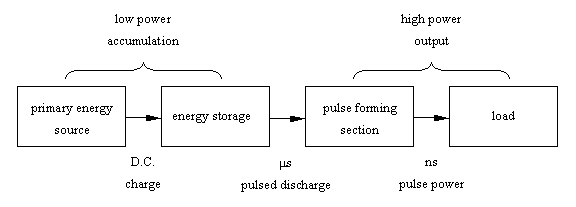
\includegraphics[height=4cm,width=8cm,keepaspectratio=true]{HPMsystem}
 \caption{Primjer ubacivanja slike}
 \label{fig:prva}
	\end{center}
\end{figure}

Znak \verb|~| iza rije�i Slici osigurava to�no jedan znak razmaka, �to poma�e ukoliko je rij�e Slika na kraju retka, da ne razdvoji rije� Slika i pripadaju�i broj slike.
Parametri slike \emph{width} i \emph{height} odre�uju maksimalne dopu�tene dimenzije pri �emu se primarno po�tuje manju navedenu dimenziju, a \emph{keepaspectratio} osigurava zadr�avanje odnosa dimenzija slike, odnosno sprje�ava deformaciju slike, nakon proizvoljno unesenih veli�ina.

Uo�i da sve oznake tj.\ \emph{labeli} ne smiju imati razmak u imenu. To vrijedi i op�enito, a ne samo za slike.

Tako�er, uo�i da nije potrebno pisati ekstenziju slike jer to je ure�eno u postavkama glavnoga dokumenta pa time �tedi trud. Ekstenzije koje se mo�e izostaviti su: \emph{jpg}, \emph{jpeg}, \emph{png} i \emph{pdf}.

Shema prikazana na Slici~\ref{fig:prva} �e biti kori�tena i za potrebe idu�ih primjera, a {\color{blue} u mapi na va�em disku ju obri�ite nakon �to po�nete pohranjivati vlastite slike vezane uz va� rad}.


\section{Ubacivanje podslika}
%
\begin{figure}[!htpb]
	  \begin{center}
	   \subfloat[kra�i opis podslike a]{\label{fig:HPM_a} 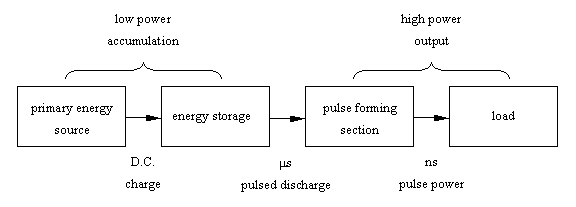
\includegraphics[height=5cm,width=8cm,keepaspectratio=true]{HPMsystem}} \\ %\hspace{10pt}
	   \subfloat[kra�i opis podslike b]{\label{fig:HPM_b} 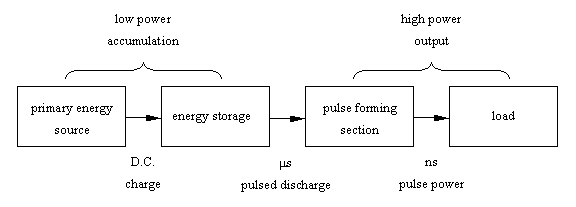
\includegraphics[height=5cm,width=8cm,keepaspectratio=true]{HPMsystem}}
\caption{Primjer ubacivanja vi�e podslika. Ovo je opis cijele slike.}
\label{fig:HPMsystem_2}
	  \end{center}
\end{figure}

Na Slici~\ref{fig:HPMsystem_2} su prikazane dvije podslike. 
Podslika~\ref{fig:HPM_a} pokazuje shemu HPM sustava, a podslika~\ref{fig:HPM_b} -- to isto.


\section{Ubacivanje tabele} \label{tabela}
Vi�e detalja o kreiranju tabela pro�itajte u literaturi, a sljede�i blok vam omogu�ava kreiranje jednostavne tabele, kao �to je prikazano u Tabeli~\ref{tab:prva}.
\begin{table}[!htbp]
\caption{Ovo je primjer izrade tabele}
\centering
\begin{tabular}{|c|c|c|}
\hline
variabla & vrijednost 1 & vrijednost 2  \\ [0.5ex]
\hline \hline  
A & 5 & 3 \\ [0.5ex]
B & 4 & 2 \\ [0.5ex]
\hline
\end{tabular}
\label{tab:prva}
\end{table}

Podaci koji su u stupcima se u tabeli razdvajaju znakom \&. Novi redak se na kraju aktualnoga retka formira znakom \verb|\\|. Broj stupaca se definira iza \emph{tabular} time �to se navedu slova koja ozna�avaju poravnavanje teksta u svakom stupcu, a broj slova zna�i broj stupaca koji �e biti kreiran u tabeli.


\section{Referenca na literaturu, sekciju, stranicu}
Na pojedinu se literaturu jednostavno uputi kori�tenjem naredbe \verb|\cite{bitex_key}| gdje je \emph{bibtex\_key} identifikator te bibliografske jedinice u bibtex datoteci. Npr.\ \verb|\cite{latex}| �e u tekstu pokazati broj te bibliografske jedinice u uglatoj zagradi \cite{latex}, te ju s istim brojem uvrsiti u popis literature (Bibliografiju) na kraju rada.

Ako se �elimo referirati na tekst u nekoj drugoj sekciji, kao npr. na dio gdje se opisuje kreiranje tabele, tada kraj te sekcije stavimo oznaku \verb|\label{ID}|, npr.\ \verb|\label{tabela}|, a na �eljenom mjestu u tekstu se na to referiramo pomo�u \verb|\ref{ID}|, npr.\ \verb|\ref{tabela}|. Tako mo�emo onda napisati da je kreiranje tabele opisano u Sekciji~\verb|~\ref{tabela}|, �to proizvede tekst koji glasi ``u Sekciji~\ref{tabela}''.

Ako �elimo navesti stranicu u na�em radu u kojoj se nalazi neki dio informacije o kojem govorimo, tada na isti na�in primijenimo \verb|\label{ID}| oznaku, a za referiranje na tu stranicu koristimo sintaksu \verb|\pageref{ID}|. 
Tako npr.\ mo�emo re�i da je primjer kreiranja tabele opisan na stranici~\verb|\pageref{tabela}|, �to �e za rezultat ima tekst u kojem pi�e da je primjer kreiranja tabele ``opisan na stranici~\pageref{tabela}''.

\section{Nagla�avanje teksta}
\subsection{Navodnici}
Za navodnike s lijeve strane fraze (otvaranje navodnika) koristi se 2x jednostruki navodnik koji se na tipkovnici nalazi lijevo od broja 1, a za navodnike s desne strane fraze (zatvaranja navodnika) se koristi 2x jednostruki navodnik koji se na tipkovnici nalazi na tipki \emph{�}, �to proizvede npr.\ ``abc''.

Alternativno, u ovom paketu je pripremljena i naredba \verb|\navod{abc}| gdje je \emph{abc} tekst koji se stavlja izme�u navodnika, tj.\ \navod{abc}.

\subsection{Kosa i podebljana slova}
Nagla�eni tekst (sli�no kosim slovima) mo�emo dobiti uporabom naredbe \verb|\emph{abc}| gdje je \emph{abc} neki tekst koji se �eli naglasiti.

Kosa slova (italic) mo�emo dobiti uporabom naredbe \verb|\textit{abc}| gdje je \textit{abc} neki tekst koji se �eli naglasiti.

Podebljana slova mo�emo posti�i uporabom naredbe \verb|\textbf{abc}| gdje je \textbf{abc} neki tekst koji �elimo podebljati.

\section{Verbatim okru�enje}
Verbatim okru�enje omogu�ava ispis teksta u izvornom obliku, bez da ga \LaTeX~ tuma�i po svojoj default sintaksi. To je pogodno kada se npr.\ na stranicu �eli kopirati dio programskoga koda iz nekog jezika i �elimo zadr�ati sve izvorne znakove, a ne da \LaTeX po�ne javljati pogre�ke kod kompajliranja jer �e ih bez toga interpretirati kao pogre�ke u sintaksi.

Postoji kra�i i du�i oblik verbatima. Kra�i slu�i za kra�u frazu od jedne ili par rije�i, a du�i za vi�e redaka.

Kra�i ima sintaksu: \verb+\verb|neka fraza|+

Du�i ima sintaksu:\\
\verb|\begin{verbatim}| \\
\verb|neki tekst| \\
\verb|\end{verbatim}| \\


\section{Kreiranje jedne jednad�be ili serije jednad�ba}

\subsection{Kreiranje jedne jednad�be}
Jednad�ba se napi�e u posebnom matemati�kom modu koji se kreira pomo�u bloka:
\begin{equation}
 A = B + C   \label{eq:prva}
\end{equation}

Jednad�ba~\eqref{eq:prva} je jedna jednostavna numerirana jednad�ba. Ako ju se ne �eli numerirati, onda se nakon rije�i \emph{begin} stavi zvjezdica, tj.\ \emph{begin\*}.

\subsection{Kreiranje vi�e jednad�ba}
Vi�e se jednad�ba kreira \emph{subequations} blokom:
\begin{subequations}
Dvije jednad�be mogu npr.\ glasiti:
\begin{align}
        A &= B + C  				\label{subeq:prva} \\
        D &= F + G				  \label{subeq:druga}
\end{align}
\label{subeq:obje}
\end{subequations}

U \eqref{subeq:prva} je prikazano dobivanje vrijednosti $A$, a u \eqref{subeq:druga} je prikazano dobivanje vrijednosti $D$. Jed.~\eqref{subeq:obje} je �uveni studentov zakon!

\section{Liste}
Liste su �este forme u tekstu kojima se na pregledni na�in nabrajaju neke stavke. Stavke obi�no navodimo s to�kama na po�etku, ili s brojevima ili sa slovima. U \LaTeX~u su upravo ta tri stila unaprijed definirana, a mogu�e su i slo�enije definicije stilova i kombinacije lista.

\subsection{Lista s to�kama}
Lista s to�kama se postigne blokom
\begin{verbatim}
\begin{itemize}
	\item prva stavka
	\item druga stavka
\end{itemize}
\end{verbatim}
�to na ekranu proizvede:
\begin{itemize}
	\item prva stavka
	\item druga stavka
\end{itemize}

\subsection{Numerirana lista s brojevima}
Numerirana lista s brojevima se postigne blokom
\begin{verbatim}
\begin{enumerate}
	\item prva stavka
	\item druga stavka
\end{enumerate}
\end{verbatim}
�to na ekranu proizvede:
\begin{enumerate}
	\item prva stavka
	\item druga stavka
\end{enumerate}


\subsection{Slov�ano numerirana lista}
Takva se lista mo�e posti�i u sklopu op�enitije forme koja omogu�uje proizvoljni opis ispred pojedine stavke, pomo�u sljede�ega bloka:
\begin{verbatim}
\begin{description}
	\item[a)] prva stavka
	\item[b)] druga stavka
\end{description}
\end{verbatim}
�to na ekranu proizvede:
\begin{description}
	\item[a)] prva stavka
	\item[b)] druga stavka
\end{description}



\section{Zavr�ne napomene}
Ovime zaklju�ujemo upute koje �e najve�em broju studenata biti dovoljne (ili barem dovoljna osnova) za uspje�no pisanje Zavr�noga odnosno Diplomskoga rada.

Prije nego prije�ete na kreiranje vlastitoga sadr�aja u�inite sljede�e:
\begin{enumerate}
	\item u mapi \href{run:slike}{{\color{blue}slike}}, obri�ite datoteku \verb|HPMsystem.png| jer je ona samo slu�ila za ilustracije u uputama
	%
	\item u glavnoj datoteci  \href{run:JMBAG\_Ime\_Prezime.tex}{{\color{blue}JMBAG\_Ime\_Prezime.tex}} stavite znak komentare ``\%'' ispred linije \verb|\chapter{Kako koristiti paket za pisanje Zavr�noga rada u \LaTeX-u}
Ovo su uvodne napomene za kori�tenje predlo�ka za pisanje Zavr�noga ili Diplomskoga rada studenata Tehni�koga fakulteta u Rijeci.

Paket je pripremljen tako da student �to prije mo�e pisati vlastiti tekst u ve� pripremljenom predlo�ku koji �e, uz minimalno u�enje sintakse \LaTeX-a, studentu olak�ati urediti svoj rad. U paketu su uklju�ene potrebne upute i sintakti�ke strukture koje bi trebale udovoljiti potrebama ve�ine studenta, a dodatne informacije postoje u priru�nicima odnosno na web stranicama na internetu koje su posve�ene \LaTeX-u (vidi u nastavku).

{\color{red} POZOR: paket treba biti prekopiran negdje na disk ne mijenjaju�i originalnu strukturi mapa (foldera) i ne mijenjaju�i nazive datoteka koje su u mapi \emph{tex\_aux}!}

\section{Opis sadr�aja paketa}
Paket se sastoji od
\begin{itemize}
 \item datoteke \href{UPUTE.pdf}{\emph{UPUTE.pdf}} koja sadr�i postupak instalacije potrebnih alata na ra�unalo te kori�tenja paketa. \emph{UPUTE} su bazirane na Windows OS, a korisnici drugih OS si na nazna�enim web lokacijama samo trebaju na�i instalacije za njihov OS.
 \item \verb|JMBAG_Ime_Prezime.tex| datoteke koja je sredi�nja datoteka koja povezuje sve cjeline i kompajliranjem koje se dobije izlazni \verb|JMBAG_Ime_Prezime.pdf| dokument.\\ U ovoj se datoteci inicijalno nalaze i upute za kori�tenje paketa kao i primjeri osnovne uporabe naj�e��ih sintakti�kih struktura u \LaTeX-u koje bi trebale biti dovoljne ve�ini studenata za pisanje rada.
 %
 \item \verb|tex_aux| mape u kojoj su interne datoteke koje definiraju stilove i dr. Student s njima ne treba \emph{ni�ta} raditi, ali one trebaju biti u \verb|tex_aux| mapi pod glavnom mapom Zavr�noga rada, kao �to je postavljeno u ovom paketu
 %
 \item mape \emph{slike} u koju student treba pohraniti sve slike koje �e koristiti u radu. Ime mape se ne smije preimenovati bez boljega poznavanja sintakse \LaTeX-a jer ovaj paket da bi ispravno radio o�ekuje ba� takvo ime mape
 %
 \item datoteke \verb|sintaksa_cestih_struktura.tex| koja ne sudjeluje izravno u kompajliranju pdf dokumenta, nego slu�i kao repozitorij u kojem su sadr�ane naj�e��e potrebne sintakti�ke strukture koje su spremne za kopiranje uz minimalnu prilagodbu parametara u studentovu radu
 %
 \item mape \href{run:manuals}{{\color{blue}manuals}} u kojoj se nalazi nekoliko najpopularnijih priru�nika za uporabu \LaTeX-a. 
\end{itemize}
%%%%%%%%%%%%%%%%%%%%%%%%%%%%%%%%%%%%%%%%%%%%%%%%%%%%%%%%%%%%%%%

\section{�ime se opremiti za pisanje rada}
Da bi se rad napisao pomo�u \LaTeX-a (a vrijedi svake lipe!), najprije je na ra�unalo potrebno instalirati (barem) \LaTeX~ software, a uz to, premda nije nu�an za pisanje rada, preporu�am i \emph{JabRef} software koji pomo�u intuitivnih su�elja korisniku omogu�ava kreiranje popisa literature na vrlo sofisticirani na�in. 

\subsection{Instalacija \LaTeX-a}
\begin{enumerate}
	\item odite na sredi�nji \LaTeX~ portal: \url{http://www.latex-project.org/}
	\item kliknite na poveznicu \href{http://www.latex-project.org/ftp.html}{Getting LaTeX} i potom uo�ite i povucite instalaciju koja odgovara va�em OSu (npr.\ proTeXt za Windows, MacTeX za Mac, TeX Live za Linux). Pozor: download je velik i mo�e du�e potrajati �ak i na brzoj vezi---dajte si dovoljno vremena za obaviti download.
	\item Instalirajte \LaTeX~ nabavljen u prethodnoj to�ki slijede�i upute koje su date za tu instalaciju (npr. proTeXt za Windowse daje kratki pdf s uputama koje vas vode kroz instalaciju korak po korak).
	\item Instalirajte si tekst-editor koji je pogodan za pisanje \LaTeX~ koda (npr.\ za Windows je popularan TeXnicCenter i dolazi ve� upakiran u proTeXt-u, za Mac je kvalitetan TeXShop koji sada tako�er dolazi u paketu s MacTeX-om).
\end{enumerate}

\subsection{Instalacija \emph{JabRef} softvera}
\emph{JabRef} je legalno besplatno dostupni softver za Windows OS (za druge OS �ete isto na�i takve programe) koji nam omogu�ava opisivanje literature na lak na�in pomo�u intuitivnih su�elja, a kao rezultat kreira \emph{BibTeX} datoteku \emph{ime.bib} (gdje je \emph{ime} koje korisnik proizvoljno dodijeli pri pohrani) u kojoj je literatura opisana na na�in koji \LaTeX~ razumije i na osnovi toga automatski formira popis literature na kraju na�ega rada, a sukladno redoslijedu pozivanja pojedine literature u tekstu.

\emph{Napomena: Kori�tenje BiBTeX programa kakav je \emph{JabRef} nije neophodno, ali prakti�no je. Alternativni---lo�iji---na�in jest ru�no opisati kori�tenu literaturu unutar \emph{tex} datoteke.\\ U datoteci po imenu \href{run:Literatura.tex}{{\color{blue}Literatura.tex}} koja je uklju�ena u ovaj paket ve� su namje�tene postavke kao da �e se literatura opisati pomo�u BiBTeX programa (npr.\ JabRef) i ne treba ni�ta mijenjati, a ispod toga se mo�e pro�itati upute i za drugi na�in (p)opisivanja literature.}

Instalacijska datoteka za \emph{JabRef} se mo�e prona�i na webu na adresi \url{http://jabref.sourceforge.net/}.
Preporu�eni postupak:
\begin{enumerate}
	\item povucite si i instalirajte posljednju stabilnu verziju \emph{JabRef}-a
	\item inicijalno se upoznajte s najva�nijim opcijama u \emph{JabRef}-u:
	\begin{enumerate}
		\item uo�ite ikonu (pod znakom ``+'' i tekstom \emph{New BibTeX Entry}) za unos nove jedinice literature (npr. knjige, �lanka, web portala i sl.)
		\item kada kliknete za unos nove stavke literature, uo�ite kakvi se sve tipovi literature nude za odabir. Odabirom opcije koja odgovara naslovu koji �elite unijeti, otvorit �e vam se novi prozor s poljima u koja se mo�e unijeti informacije o literaturi. Za odabrani tip literature samo su neka polja obavezna (nalaze se pod karticom (eng.\ \emph{tabom}) \emph{Required fields}), dok se pod drugim karticama mo�e i ne mora unijeti dodatne informacije.
		\item prije nego pohranite va� unos sa \emph{Ctrl+S}, morate toj jedinici dodijeliti jedinstveni identifikator, tzv.\ \emph{Bibtexkey}, �to je jedno od polja koja su obavezna za unos. Mo�ete ru�no upisati neki proizvoljni string, ali pogodnije je generirati ga automatski. Za to u�initi me�u ikonama na vrhu imate ikonu koja izgleda kao (�arobni) �tapi� sa zvjezdicama oko njega, klikom na kojega \emph{JabRef} automatski dodijeli jedinstveni BibTeX \emph{klju�} za tu bibliografsku jedinicu. Pomo�u toga klju�a se poslije bilo kada i bilo gdje u pisanju va�ega rada mo�ete pozvati na tu referencu, a \LaTeX~ �e sve ostalo obaviti za vas tj.\ dodijeliti joj odgovaraju�i broj u tekstu i s tim brojem uvrstiti u popis literature.
		\item korisnik ima mogu�nost i promijeniti uzorak po kojem se kreira struktura automatski generiranoga jedinstvenoga BibTeX klju�a tako da se ode u opciju izbornika \emph{Options $>>$ Preferences $>>$ BibTeX key generator} gdje je na vrhu prozora prikazan \emph{default} uzorak, npr. \verb|[auth]:[year]| �to zna�i da se klju� kreira na bazi \verb|prezime(autora):godina(rada)|. To se sada mo�e urediti po nekom novom uzorku, no ovako definirani uzorak u biti zadovoljava, a ako igdje ima potrebe za dodatnim razlikovanjem, mo�e se automatski generiran klju� jo� ru�no napraviti korekcija dodavanjem na kraju npr.\ \verb|_a| itd.
		\item klikom na karticu \emph{BibTeX source} mo�ete vidjeti kako �e unos va�ih podataka zapravo biti zapisan u va�oj \emph{ime.bib} datoteci koja �e se formirati od svih bibliografskih jedinica koje unesete.
		\item Za \emph{ime} va�e bibliografske datoteke kod pohrane odaberite \emph{Literatura} jer to ime o�ekuje ovaj paket. Ina�e se mo�e dodijeliti proizvoljno ime, ali onda treba znati �to i gdje promijeniti u sredi�njoj \LaTeX~ datoteci. Pozor: Datoteka \emph{Literatura.bib} koju ste tako kreirali mora se nalaziti unutar mape ovoga paketa da bi sve ispravno radilo! U paketu je za primjer ve� kreirana jedna datoteka istoga imena koju za vje�bu student mo�e i otvoriti u \emph{JabRef}-u, ali to su samo pokazne bibliografske jedinice unesene kao primjer, koje student treba u kona�nici zamijeniti svojim stvarnim podacima.
	\end{enumerate}
\end{enumerate} 
%%%%%%%%%%%%%%%%%%%%%%%%%%%%%%%%%%%%%%%%%%%%%%%%%%%

\section{Kako (kona�no) po�eti pisati svoj rad}
Najbr�i start je sljede�i:
\begin{enumerate}
	\item Pokrenite va� \LaTeX~tekst-editor i iz njega otvorite pripremljeni predlo�ak za pisanje rada \href{run:JMBAG_Ime_Prezime.tex}{{\color{blue}JMBAG\_Ime\_Prezime.tex}} koji se nalazi unutar ovoga paketa (obi�no ga se mo�e otvoriti i dvostrukim klikom na \emph{tex} datoteku ukoliko �e OS koristiti \LaTeX~ editor za otvaranje iste)
	\item skrolajte niz dokumentu ni�ta ne mijenjaju�i, dok ne nai�ete na retke u kojima su kratke upute koje upu�uju studenta �to treba upisati u pripremljenu naredbu. U biti, u gornjem dijelu dokumenta nema u biti ni�ega za mijenjati, nego tek nakon linije koja sadr�i \verb|\begin{document}|. Specifi�ni podaci koje student treba upisati bit �e uz naredbe:
	%
		\begin{itemize}
			\item \verb|\degreesubject|: upisati vrstu studija (preddiplomski ili diplomski studij studentovoga usmjerenja)
			\item \verb|\documenttype|: upisati \emph{Zavr�ni rad} ili \emph{Diplomski rad}
			\item \verb|\title|: upisati naslov rada
			\item \verb|\date|: upisati samo mjesec predaje rada. Godina se upisuje automatski.
			\item \verb|\author|: upisati ime i prezime studenta
			\item \verb|\jmbag|: zamijeniti postoje�i broj vlastitim JMBAG brojem 
			\item \verb|\mentor|: upisati titulu i ime i prezime svojega mentora
		\end{itemize}
	%
	\item Za prvu probu nakon une�enih podataka, kompajlirajte dokument na na�in da unutar va�ega tekst-editora odaberete opciju izbornika (odnosno ikonu) koja glasi ne�to poput \emph{Build and View (Current File)}. To pokrene postupak kompajliranja svega i rezultat bi trebao biti \emph{pdf} datoteka u kojoj �ete vidjeti lijepo formatirane po�etne stranice rada. Pozor: 
		\begin{itemize}
			\item provjerite u postavkama editora da je izlazni format PDF. To se ili vidi negdje na ekranu va�ega editora ili negdje pod opcijom koja glasi poput \emph{Select Output Profile} (vjerojatno pod \emph{Build} izbornikom) i nudi par izlaznih formata jedan od kojih je PDF.
			\item nekada je potrebno 2-3 puta pokrenuti \emph{Build} operaciju da bi sve promjene bile a�urirane u \emph{pdf} dokumentu kao �to su npr.\ brojevi referenca, popis literature i sl.
		\end{itemize}
		%
	\item Za (i vi�e nego) osnovnu sintaksu mo�ete otvoriti datoteku \href{run:Intro.tex}{{\color{blue}Intro.tex}} koja je dio paketa i unutar koje su napisane i ove upute. Vidjet �ete da da se odmah mo�e pisati va� tekst uz nekoliko osnovnih naredaba, kao �to su:
	\begin{itemize}
		\item \verb|\chapter{Naslov poglavlja}| kojim definirate naslov poglavlja
		\item \verb|\section{Naslov sekcije}| kojim definirate naslov sekcije unutar poglavlja
		\item \verb|\subsection{Naslov podsekcije}| kojim definirate naslov podsekcije
		\item \verb|\cite{bibtexkey}| kojom se pozivate na odre�enu literaturu jedinstveni klju� koje je u BibTeX datoteci \href{run:Literatura.bib}{{\color{blue}Literatura.bib}} dan sa \emph{bibtex key}
		\item \verb|\emph{tekst}| naredbu kojom se pomo�u italic slova nagla�ava neka rije� ili fraza
		\item \verb|\href| ili \verb|\url| naredba kojom se kreira poveznica na neku URL adresu ili dokument (ne pretjerujte s tim, odnosno uop�e ne morate to koristiti u radu, nego za vanjske reference koristiti samo \verb|\cite{}| naredbu, a za unutra�nje reference (na dijelove teksta) kombinaciju naredbi \verb|\label{ID}| i \verb|\ref{ID}| gdje se prvu postavi na dio teksta na koji �emo se poslije referencirati, a drugu na mjestu s kojega se referenciramo)
		\item ostale sintakse kao �to su ubacivanje slike, tabele ili jednad�ba mo�ete na�i u datoteci \href{run:sintaksa_cestih_struktura.tex}{{\color{blue}sintaksa\_cestih\_struktura.tex}} koja je dio paketa. Odabrane se strukture mo�e kopirati i zalijepiti u va� tekst, uz minimalne prilagodbe kao �to su naziv slike, veli�ina slike, opis i ID slike, a analogno i za tabele i jednad�be.
		\item Kona�no, za vi�e detalja o bilo �emu, potra�ite informacije u priru�nicima koji su prilo�eni u mapi \href{run:manuals}{{\color{blue}manuals}} ili na webu, gdje se, me�u obiljem drugih informacija, nalaze i korisne \href{http://en.wikibooks.org/wiki/LaTeX/}{wiki stranice} o \LaTeX-u pomo�u kojih se obi�no brzo prona�e upute i zadovoljavaju�e rje�enje kojom sintaksom se mo�e urediti �eljeni dio teksta.
  	\end{itemize}
\item Savjet: svako poglavlje napi�ite u novoj datoteci koju imenujte prikladnim imenom (bez razmaka u imenu) i potom ih samo pozivajte iz glavnoga dokumenta \emph{JMBAG\_Ime\_Prezime.tex} pomo�u \verb|\include{ime_datoteke}| naredbe.
\end{enumerate}

Nadam se da �e vam ovaj dokument pomo�i u pripremi teksta va�ega rada i omogu�iti tro�iti glavninu vremena na sadr�aj rada, a manje na formatiranje rada jer to bi za vas sada trebao obaviti \LaTeX! 
No, fair-playa radi, potrebno je napomenuti i sljede�e: \LaTeX~ je vrlo osjetljiv na pogre�ke u sintaksi naredbi (da, ba� kao svaki programski jezik) pa vas mo�e povremeno zagnjaviti javljanjem pogre�ke koju nikako ne uspijevate uo�iti gdje je. Iskustvo kojim se izbjegava ta nelagoda jest sljede�e:
\begin{itemize}
	\item budite koncentrirani dok pi�ete \LaTeX~naredbe
	\item kompajlirajte tekst prije nego se skupi puno teksta jer tako �ete imati manje teksta za prekontrolirati u slu�aju pogre�ke
	\item ako niste sigurni ho�e li vam raditi neka naredba nakon pisanja, radije odmah kompajlirajte tekst da vidite �to �ete dobiti i rije�ite dvojbu, nego �ekati da se skupi jo� dubioza, kada �e biti te�e detektirati koja naredba zapravo izaziva probleme (\LaTeX~ov prozor s porukama nije odve� precizan u lociranju i opisu pogre�aka)
\end{itemize}

%%%%%%%% POGLAVLJE ZAVRSENO %%%%%%%%%%%%%%%


\chapter{Primjeri naj�e��ih sintakti�kih struktura}
Ovo se poglavlje u ovome trenutku i ne mora �itati, ali za one koje se �ele bolje pripremiti prije samoga po�etka pisanja rada, sigurno �e pomo�i. 

U nastavku su opisane naj�e��e sintakti�ke strukture, a koje za budu�e potrebe imate pohranjene i u datoteci \href{run:sintaksa_cestih_struktura.tex}{{\color{blue}sintaksa\_cestih\_struktura.tex}} koja je sastavni dio glavne mape ovoga paketa.

\section{Ubacivanje slike}
Na Slici~\ref{fig:prva} je prikazana osnovna shema HPM sustava.
\begin{figure}[!htbp]
	\begin{center}
 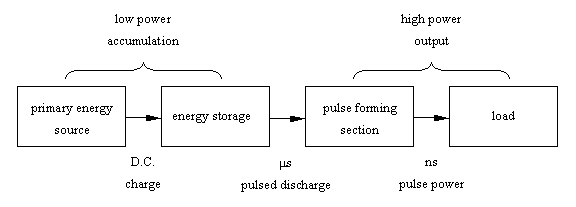
\includegraphics[height=4cm,width=8cm,keepaspectratio=true]{HPMsystem}
 \caption{Primjer ubacivanja slike}
 \label{fig:prva}
	\end{center}
\end{figure}

Znak \verb|~| iza rije�i Slici osigurava to�no jedan znak razmaka, �to poma�e ukoliko je rij�e Slika na kraju retka, da ne razdvoji rije� Slika i pripadaju�i broj slike.
Parametri slike \emph{width} i \emph{height} odre�uju maksimalne dopu�tene dimenzije pri �emu se primarno po�tuje manju navedenu dimenziju, a \emph{keepaspectratio} osigurava zadr�avanje odnosa dimenzija slike, odnosno sprje�ava deformaciju slike, nakon proizvoljno unesenih veli�ina.

Uo�i da sve oznake tj.\ \emph{labeli} ne smiju imati razmak u imenu. To vrijedi i op�enito, a ne samo za slike.

Tako�er, uo�i da nije potrebno pisati ekstenziju slike jer to je ure�eno u postavkama glavnoga dokumenta pa time �tedi trud. Ekstenzije koje se mo�e izostaviti su: \emph{jpg}, \emph{jpeg}, \emph{png} i \emph{pdf}.

Shema prikazana na Slici~\ref{fig:prva} �e biti kori�tena i za potrebe idu�ih primjera, a {\color{blue} u mapi na va�em disku ju obri�ite nakon �to po�nete pohranjivati vlastite slike vezane uz va� rad}.


\section{Ubacivanje podslika}
%
\begin{figure}[!htpb]
	  \begin{center}
	   \subfloat[kra�i opis podslike a]{\label{fig:HPM_a} 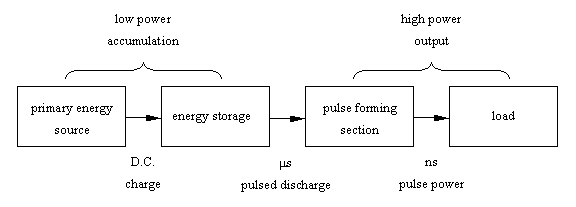
\includegraphics[height=5cm,width=8cm,keepaspectratio=true]{HPMsystem}} \\ %\hspace{10pt}
	   \subfloat[kra�i opis podslike b]{\label{fig:HPM_b} 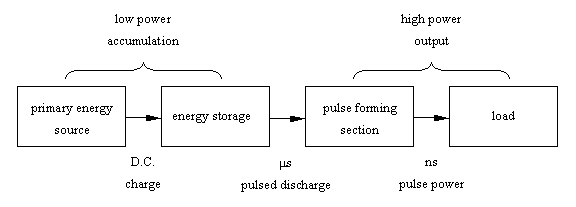
\includegraphics[height=5cm,width=8cm,keepaspectratio=true]{HPMsystem}}
\caption{Primjer ubacivanja vi�e podslika. Ovo je opis cijele slike.}
\label{fig:HPMsystem_2}
	  \end{center}
\end{figure}

Na Slici~\ref{fig:HPMsystem_2} su prikazane dvije podslike. 
Podslika~\ref{fig:HPM_a} pokazuje shemu HPM sustava, a podslika~\ref{fig:HPM_b} -- to isto.


\section{Ubacivanje tabele} \label{tabela}
Vi�e detalja o kreiranju tabela pro�itajte u literaturi, a sljede�i blok vam omogu�ava kreiranje jednostavne tabele, kao �to je prikazano u Tabeli~\ref{tab:prva}.
\begin{table}[!htbp]
\caption{Ovo je primjer izrade tabele}
\centering
\begin{tabular}{|c|c|c|}
\hline
variabla & vrijednost 1 & vrijednost 2  \\ [0.5ex]
\hline \hline  
A & 5 & 3 \\ [0.5ex]
B & 4 & 2 \\ [0.5ex]
\hline
\end{tabular}
\label{tab:prva}
\end{table}

Podaci koji su u stupcima se u tabeli razdvajaju znakom \&. Novi redak se na kraju aktualnoga retka formira znakom \verb|\\|. Broj stupaca se definira iza \emph{tabular} time �to se navedu slova koja ozna�avaju poravnavanje teksta u svakom stupcu, a broj slova zna�i broj stupaca koji �e biti kreiran u tabeli.


\section{Referenca na literaturu, sekciju, stranicu}
Na pojedinu se literaturu jednostavno uputi kori�tenjem naredbe \verb|\cite{bitex_key}| gdje je \emph{bibtex\_key} identifikator te bibliografske jedinice u bibtex datoteci. Npr.\ \verb|\cite{latex}| �e u tekstu pokazati broj te bibliografske jedinice u uglatoj zagradi \cite{latex}, te ju s istim brojem uvrsiti u popis literature (Bibliografiju) na kraju rada.

Ako se �elimo referirati na tekst u nekoj drugoj sekciji, kao npr. na dio gdje se opisuje kreiranje tabele, tada kraj te sekcije stavimo oznaku \verb|\label{ID}|, npr.\ \verb|\label{tabela}|, a na �eljenom mjestu u tekstu se na to referiramo pomo�u \verb|\ref{ID}|, npr.\ \verb|\ref{tabela}|. Tako mo�emo onda napisati da je kreiranje tabele opisano u Sekciji~\verb|~\ref{tabela}|, �to proizvede tekst koji glasi ``u Sekciji~\ref{tabela}''.

Ako �elimo navesti stranicu u na�em radu u kojoj se nalazi neki dio informacije o kojem govorimo, tada na isti na�in primijenimo \verb|\label{ID}| oznaku, a za referiranje na tu stranicu koristimo sintaksu \verb|\pageref{ID}|. 
Tako npr.\ mo�emo re�i da je primjer kreiranja tabele opisan na stranici~\verb|\pageref{tabela}|, �to �e za rezultat ima tekst u kojem pi�e da je primjer kreiranja tabele ``opisan na stranici~\pageref{tabela}''.

\section{Nagla�avanje teksta}
\subsection{Navodnici}
Za navodnike s lijeve strane fraze (otvaranje navodnika) koristi se 2x jednostruki navodnik koji se na tipkovnici nalazi lijevo od broja 1, a za navodnike s desne strane fraze (zatvaranja navodnika) se koristi 2x jednostruki navodnik koji se na tipkovnici nalazi na tipki \emph{�}, �to proizvede npr.\ ``abc''.

Alternativno, u ovom paketu je pripremljena i naredba \verb|\navod{abc}| gdje je \emph{abc} tekst koji se stavlja izme�u navodnika, tj.\ \navod{abc}.

\subsection{Kosa i podebljana slova}
Nagla�eni tekst (sli�no kosim slovima) mo�emo dobiti uporabom naredbe \verb|\emph{abc}| gdje je \emph{abc} neki tekst koji se �eli naglasiti.

Kosa slova (italic) mo�emo dobiti uporabom naredbe \verb|\textit{abc}| gdje je \textit{abc} neki tekst koji se �eli naglasiti.

Podebljana slova mo�emo posti�i uporabom naredbe \verb|\textbf{abc}| gdje je \textbf{abc} neki tekst koji �elimo podebljati.

\section{Verbatim okru�enje}
Verbatim okru�enje omogu�ava ispis teksta u izvornom obliku, bez da ga \LaTeX~ tuma�i po svojoj default sintaksi. To je pogodno kada se npr.\ na stranicu �eli kopirati dio programskoga koda iz nekog jezika i �elimo zadr�ati sve izvorne znakove, a ne da \LaTeX po�ne javljati pogre�ke kod kompajliranja jer �e ih bez toga interpretirati kao pogre�ke u sintaksi.

Postoji kra�i i du�i oblik verbatima. Kra�i slu�i za kra�u frazu od jedne ili par rije�i, a du�i za vi�e redaka.

Kra�i ima sintaksu: \verb+\verb|neka fraza|+

Du�i ima sintaksu:\\
\verb|\begin{verbatim}| \\
\verb|neki tekst| \\
\verb|\end{verbatim}| \\


\section{Kreiranje jedne jednad�be ili serije jednad�ba}

\subsection{Kreiranje jedne jednad�be}
Jednad�ba se napi�e u posebnom matemati�kom modu koji se kreira pomo�u bloka:
\begin{equation}
 A = B + C   \label{eq:prva}
\end{equation}

Jednad�ba~\eqref{eq:prva} je jedna jednostavna numerirana jednad�ba. Ako ju se ne �eli numerirati, onda se nakon rije�i \emph{begin} stavi zvjezdica, tj.\ \emph{begin\*}.

\subsection{Kreiranje vi�e jednad�ba}
Vi�e se jednad�ba kreira \emph{subequations} blokom:
\begin{subequations}
Dvije jednad�be mogu npr.\ glasiti:
\begin{align}
        A &= B + C  				\label{subeq:prva} \\
        D &= F + G				  \label{subeq:druga}
\end{align}
\label{subeq:obje}
\end{subequations}

U \eqref{subeq:prva} je prikazano dobivanje vrijednosti $A$, a u \eqref{subeq:druga} je prikazano dobivanje vrijednosti $D$. Jed.~\eqref{subeq:obje} je �uveni studentov zakon!

\section{Liste}
Liste su �este forme u tekstu kojima se na pregledni na�in nabrajaju neke stavke. Stavke obi�no navodimo s to�kama na po�etku, ili s brojevima ili sa slovima. U \LaTeX~u su upravo ta tri stila unaprijed definirana, a mogu�e su i slo�enije definicije stilova i kombinacije lista.

\subsection{Lista s to�kama}
Lista s to�kama se postigne blokom
\begin{verbatim}
\begin{itemize}
	\item prva stavka
	\item druga stavka
\end{itemize}
\end{verbatim}
�to na ekranu proizvede:
\begin{itemize}
	\item prva stavka
	\item druga stavka
\end{itemize}

\subsection{Numerirana lista s brojevima}
Numerirana lista s brojevima se postigne blokom
\begin{verbatim}
\begin{enumerate}
	\item prva stavka
	\item druga stavka
\end{enumerate}
\end{verbatim}
�to na ekranu proizvede:
\begin{enumerate}
	\item prva stavka
	\item druga stavka
\end{enumerate}


\subsection{Slov�ano numerirana lista}
Takva se lista mo�e posti�i u sklopu op�enitije forme koja omogu�uje proizvoljni opis ispred pojedine stavke, pomo�u sljede�ega bloka:
\begin{verbatim}
\begin{description}
	\item[a)] prva stavka
	\item[b)] druga stavka
\end{description}
\end{verbatim}
�to na ekranu proizvede:
\begin{description}
	\item[a)] prva stavka
	\item[b)] druga stavka
\end{description}



\section{Zavr�ne napomene}
Ovime zaklju�ujemo upute koje �e najve�em broju studenata biti dovoljne (ili barem dovoljna osnova) za uspje�no pisanje Zavr�noga odnosno Diplomskoga rada.

Prije nego prije�ete na kreiranje vlastitoga sadr�aja u�inite sljede�e:
\begin{enumerate}
	\item u mapi \href{run:slike}{{\color{blue}slike}}, obri�ite datoteku \verb|HPMsystem.png| jer je ona samo slu�ila za ilustracije u uputama
	%
	\item u glavnoj datoteci  \href{run:JMBAG\_Ime\_Prezime.tex}{{\color{blue}JMBAG\_Ime\_Prezime.tex}} stavite znak komentare ``\%'' ispred linije \verb|\include{Intro}| kojom se pozivaju ove upute, �ime to vi�e ne�e biti uklju�eno u tekst vlastitoga rada
	%
	\item otvorite datoteku \href{run:Poglavlje\_1.tex}{{\color{blue}Poglavlje\_1.tex}} i po�nite pisati svoj vlastiti tekst uz postavljanje naslova poglavlja i sekcija po vlastitom izboru, a na kraju promijenite ime te datoteke u ne�to �to odgovara sadr�aju va�ega poglavlja i to ime stavite u \verb|\include| naredbu umjesto inicijalnoga naziva \verb|Poglavlje_1|. Kona�no, da bi se tekst toga poglavlja kompajlirao u izlazni dokument, uklonite znak komentara ``\%'' ispred te \verb|\include| naredbe. Tako u�inite i za sva nova poglavlja koja �ete potom kreirati.
\end{enumerate}


Svoje dojmove o razumljivosti i prakti�nosti ovoga materijala mo�ete emailati klikom \href{mailto:mjoler@riteh.hr}{{\color{blue}ovdje}}.

Ugodan rad!


Miroslav Joler



%%%%%  POGLAVLJE ZAVRSENO  %%%%%| kojom se pozivaju ove upute, �ime to vi�e ne�e biti uklju�eno u tekst vlastitoga rada
	%
	\item otvorite datoteku \href{run:Poglavlje\_1.tex}{{\color{blue}Poglavlje\_1.tex}} i po�nite pisati svoj vlastiti tekst uz postavljanje naslova poglavlja i sekcija po vlastitom izboru, a na kraju promijenite ime te datoteke u ne�to �to odgovara sadr�aju va�ega poglavlja i to ime stavite u \verb|\include| naredbu umjesto inicijalnoga naziva \verb|Poglavlje_1|. Kona�no, da bi se tekst toga poglavlja kompajlirao u izlazni dokument, uklonite znak komentara ``\%'' ispred te \verb|\include| naredbe. Tako u�inite i za sva nova poglavlja koja �ete potom kreirati.
\end{enumerate}


Svoje dojmove o razumljivosti i prakti�nosti ovoga materijala mo�ete emailati klikom \href{mailto:mjoler@riteh.hr}{{\color{blue}ovdje}}.

Ugodan rad!


Miroslav Joler



%%%%%  POGLAVLJE ZAVRSENO  %%%%%| kojom se pozivaju ove upute, �ime to vi�e ne�e biti uklju�eno u tekst vlastitoga rada
	%
	\item otvorite datoteku \href{run:Poglavlje\_1.tex}{{\color{blue}Poglavlje\_1.tex}} i po�nite pisati svoj vlastiti tekst uz postavljanje naslova poglavlja i sekcija po vlastitom izboru, a na kraju promijenite ime te datoteke u ne�to �to odgovara sadr�aju va�ega poglavlja i to ime stavite u \verb|\include| naredbu umjesto inicijalnoga naziva \verb|Poglavlje_1|. Kona�no, da bi se tekst toga poglavlja kompajlirao u izlazni dokument, uklonite znak komentara ``\%'' ispred te \verb|\include| naredbe. Tako u�inite i za sva nova poglavlja koja �ete potom kreirati.
\end{enumerate}


Svoje dojmove o razumljivosti i prakti�nosti ovoga materijala mo�ete emailati klikom \href{mailto:mjoler@riteh.hr}{{\color{blue}ovdje}}.

Ugodan rad!


Miroslav Joler



%%%%%  POGLAVLJE ZAVRSENO  %%%%%   % ovo poslije staviti pod komentar kada se nauèi koristiti
\chapter{Uvod}

Tehnologija je sveprisutna u dana\v{s}njem svijetu. Ne postoji grana ljudske djelatnosti koja u zadnjih 30 godina nije redefinirana dolaskom elektroni\v{c}kih ure\dj aja. Danas se u sve ugra\dj uju elektroni\v{c}ki sklopovi koji pobolj\v{s}avaju i pro\v{s}iruju funkcionalnosti ure\dj aja. Sve vi\v{s}e i vi\v{s}e ure\dj aja dobiva prefiks ``pametni'', \v{s}to ozna\v{c}ava da ure\dj aj sadr\v{z}i neku vrstu mikroprocesora koji u pozadini izvr\v{s}ava neku logiku i time unaprje\dj uje ure\dj aj. \v{s}to vi\v{s}e takvih ure\dj aja postoji, to je ve\'{c}a potreba za protokolima pomo\'{c}u kojih \'{c}e ure\dj aji komunicirati sa drugim ure\dj ajima. Umre\v{z}avanjem ure\dj aja se ponovno pro\v{s}iruju njihove funkcionalnosti i dolazi do novih mogu\'{c}nosti i podru\v{c}ja primjene.

Cilj ovog rada je evaluirati i u prakti\v{c}nom primjeru implementirati dva sli\v{c}na be\v{z}i\v{c}na komunikacijska protokola, NFC (Near Field Communicaiton) i BLE (Bluetooth Low Energy). Glavni motiv odabira ovih protokola je njihova sveprisutnost -  danas gotovo svaki novi pametni telefon ima ugra\dj en NFC i BLE modul. Ako se uzme u obzir da je kori\v{s}tenje pametnog telefona postala svakodnevica gotovo polovice \v{c}ovje\v{c}anstva. Po izvje\v{s}\'{c}u ``Ericsson Mobility Report'' tvrtke Ericsson \cite{mobilityReport} 2015. godine se u svijetu koristilo 3,4 milijardi pametnih telefona, a predvi\dj eno je da \'{c}e se do 2021. ta brojka popeti do \v{c}ak 6,4 milijardi. Prema tim podacima mo\v{z}e se zaklju\v{c}iti da mobilne aplikacije koje u svojim funkcionalnostima koriste NFC ili BLE protokol imaju ogromno potencijalno tr\v{z}i\v{s}te. Ipak, treba sa rezervom uzeti toliku brojku jer se oba protokola tek po\v{c}inju ugra\dj ivati u ve\'{c}inu novih pametnih telefona, dok su ih proteklih godina proizvo\dj a\v{c}i ugra\dj ivali samo u svoje najja\v{c}e i najskuplje modele.

Sli\v{c}nost protokola je u tome \v{s}to se oba koriste za be\v{z}i\v{c}nu komunikaciju kratkog dometa. Me\dj utim, tehnologija koja se koristi za implementaciju protokola je potpuno razli\v{c}ita. NFC za prijenos podataka koristi svojstva elektromagnetske indukcije, dok se kod BLE prijenos podataka ostvaruje preko radio valova. Samim time su svojstva protokola razli\v{c}ita, najbolji primjer je domet - NFC u praksi ima domet do 5 cm, a BLE do 10 metara, \v{s}to na kraju rezultira razli\v{c}itom primjenom u praksi. Upravo zato su protokoli komplementarni i zajedno se ugra\dj uju u pametne telefone jer zajedno mogu pru\v{z}iti rje\v{s}enje za gotovo sve potrebe u kratko dometnoj komunikaciji na razini prostorije. Naravno, razlog tome je i to \v{s}to su pametni telefon vrlo napredni ure\dj aji koji osim NFC i BLE modula imaju i GSM modul, modul za mobilni internet i WiFi modul, koji nisu uvijek optimalni za komunikaciju u kratkom dometu. Me\dj utim, kombinacija svih navedenih modula i mogu\'{c}nosti protokola koje implementiraju, \v{c}ini pametni telefon ure\dj ajem bez kojeg je \v{z}ivot \v{c}ovjeka u 21. stolje\'{c}u nezamisliv.

Zbog svega navedenog, temeljna ideja ovog rada je implementirati oba protokola u sustav koji funkcionira i koji ima potencijala za\v{z}ivjeti na dana\v{s}njem tr\v{z}i\v{s}tu. Nastavak ovog poglavlja sadr\v{z}i opis sustava, aktivnosti obavljene za ostvarivanje sustava te krajnji rezultat.

   
\chapter{Specifikacija rada}

Ovaj rad za cilj ima teoretski opisati i prakti\v{c}nim primjerom testirati dva sli\v{c}na be\v{z}i\v{c}ne protokola, NFC (Near Field Communication) i BLE (Bluetooth Low Energy). Motivi za odabir ovakve teme uklju\v{c}uju relativnu , veliko podru\v{c}je primjene i razli\v{c}ite mogu\'{c} nosti koje pru\v{z}aju oba protokola. Me\dj utim, glavni motiv je sveprisutnost navedenih protokola jer danas gotovo svaki novi pametni telefon ima ugra\dj en NFC i BLE modul. Ako se uzme u obzir da je kori\v{s}tenje pametnog telefona postala svakodnevica gotovo polovice ljudi na svijetu (po izvje\v{s}\'{c} u ``Ericsson Mobility Report'' tvrtke Ericsson \cite{mobilityReport} 2015. godine se u svijetu se koristilo 3,4 milijardi pametnih telefona, a predvi\dj eno je da \'{c} e se do 2021. ta brojka popeti do \v{c}ak 6,4 milijardi), dolazi se do zaklju\v{c}ka da mobilne aplikacije koje u svojim funkcionalnostima koriste NFC ili BLE protokol imaju potencijalno ogromno tr\v{z}i\v{s}te. Ipak, treba sa rezervom uzeti toliku brojku jer se oba protokola tek po\v{c}inju ugra\dj aviti u ve\'{c} inu novih pametnih telefona, dok su ih proteklih godina proizvo\dj a\v{c}i ugra\dj ivali samo u svoje najja\v{c}e i najskuplje modele.

Sli\v{c}nost protokola je u tome \v{s}to se oba koriste za be\v{z}i\v{c}nu komunikaciju kratkog dometa. Me\dj utim, tehnologija koja se koristi za implementaciju protokola je potpuno razli\v{c}ita. NFC za prijenos podataka koristi svojstva elektromagnetske indukcije, dok se kod BLE-a prijenos podataka ostvaruje preko radio valova. Samim time su svojstva protokola razli\v{c}ita (najbolji primjer je domet - NFC u praksi ima domet do 5 cm, a BLE do 10 metara) \v{s}to na kraju rezultira razli\v{c}itom primjenom u praksi. Upravo zato su protokoli komplementarni i zajedno se ugra\dj uju u pametne telefone jer zajedno mogu pru\v{z}iti rje\v{s}enje za gotovo sve potrebe u kratko dometnoj komunikaciji (razina prostorije). Naravno, razlog tome je i to \v{s}to su pametni telefon vrlo napredni ure\dj aji koji osim NFC i BLE modula imaju i GSM modul, modul za mobilni internet i WiFi modul, koji nisu uvijek optimalni za komunikaciju u kratkom dometu. Me\dj utim, kombinacija svih navedenih modula i mogu\'{c}nosti protokola koje implementiraju, \v{c}ini pametni telefon tako naprednim ure\dj ajem bez kojeg je \v{z}ivot modernog \v{c}ovjeka u 21. stolje\'{c}u nezamisliv.

Zbog svega navedenog, temeljna ideja ovog rada je implementirati oba protokola u sustav koji ima smisla i koji ima potencijala za\v{z}ivjeti na dana\v{s}njem tr\v{z}i\v{s}tu. Nastavak ovog poglavlja sadr\v{z}i opis sustava, aktivnosti koje su poduzete za ostvarivanje sustava te krajnji rezultat.

\section{Specifikacija sustava}

Glavna ideja sustava je kreirati mobilnu aplikaciju i administrativno su\v{c}elje koje bi trgova\v{c}ki lanci koristili za promociju proizvoda u svojim poslovnicama. Ideja je da trgova\v{c}ki lanaci preko internetskog su\v{c}elja kreiraju popuste za svoje proizvode u odabranim poslovinicama, a zatim kupci pomo\'{c}u mobilne aplikacije ostvaruju kreirane popuste. Korisni\v{c}ko iskustvo je zami\v{s}ljeno tako da korisnik prilikom ulaza u poslovnicu, pomo\'{c}u pametnog telefona sa instaliranom aplikacijom te NFC i BLE modulom, skenira NFC naljepnicu koja aplikaciji daje informaciju u koju je poslovnicu korisnik u\v{s}ao. Mobilna aplikacija zatim dohva\'{c}a konfiguraciju te poslovnice poslovnice sa poslu\v{z}itelja, te je ta akcija je prikazana na slici ~\ref{fig:skeniranjeNaljepnice}.

\begin{figure}[!htbp]
	\begin{center}
 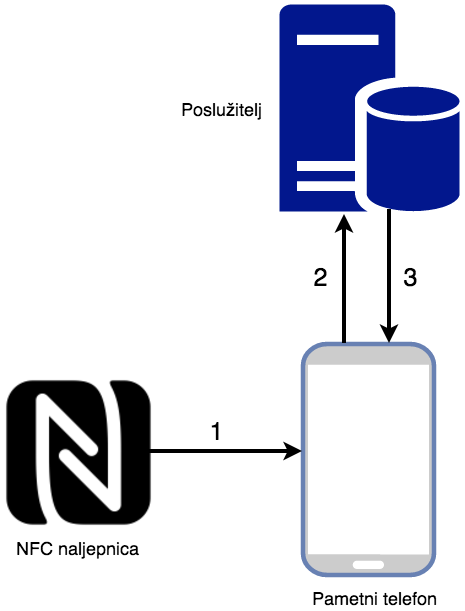
\includegraphics[height=12cm,keepaspectratio=true]{nfc_sken}
 \caption{Prikaz procesa skeniranja NFC naljepnice (1), zahtjeva za konfiguracijom poslovnice (2) i dobivanje konfiguracje poslovnice (3).}
 \label{fig:skeniranjeNaljepnice}
	\end{center}
\end{figure}

Kada je aplikacija dobila konfiguraciju po\v{c}inje sa skeniranjem okoline, s ciljem nala\v{z}enja BLE ure\dj aja. Proizvodi na akciji imaju u svojoj neposrednoj blizini BLE ogla\v{s}iva? te korisniku koji prolazi pokraj police od proizvoda, ukoliko ima upaljenu aplikaciju, prona\dj eni popust postaje vidljiv u aplikaciji. Tada, ukoliko se odlu\v{c}i na iskori\v{s}tavanje popusta, kreira zahtjev za kodom popusta. Zahtjev je vezan za korisnikov ure\dj aj (zbog za\v{s}tite od zloupotrebe - svaki ure\dj aj mo\v{z}e jedan popust ostvariti maksimalno jedan put) te korisnik dobiva kod za popust kojeg je, s ciljem ostvarivanja popusta, du\v{z}an prikazati na blagajni. Opisani postupci su prikazani na slici  ~\ref{fig:otkrivanjeBLEa}.

\begin{figure}[!htbp]
	\begin{center}
 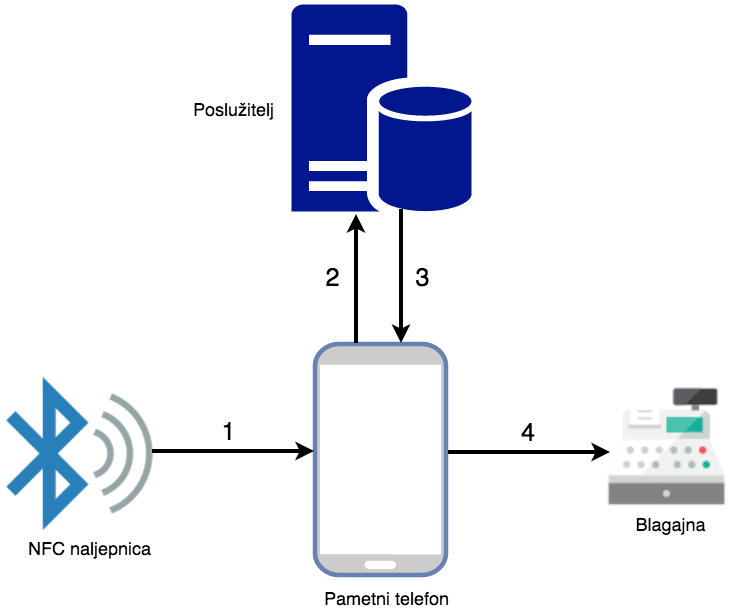
\includegraphics[height=12cm,keepaspectratio=true]{ble_sken}
 \caption{Prikaz procesa otkrivanja BLE ogla\v{s}iva\v{c}a (1), zahtjev za kodom skeniranog popusta (2), dobivanje koda za popust (3) i prikazivanje koda na blagajni za kona\v{c}no ostvarivanje popusta (4).}
 \label{fig:otkrivanjeBLEa}
	\end{center}
\end{figure}

Za implementaciju opisanog sustava potrebne su slijede\'{c}e aktivnosti:
\begin{enumerate}
	\item Kreiranje web aplikacije sa su\v{c}eljem za poslovne subjekte
	\item Kreiranje API su\v{c}elja za komunikaciju mobilne aplikacije i poslu\v{z}itelja
	\item Konfiguriranje NFC naljepnica i BLE ogla\v{s}iva\v{c}a
	\item Kreiranje mobilne aplikacije
	
\end{enumerate}

Resursi potrebni za ostvarivanje aktivnosti uklju\v{c}uju:
\begin{enumerate}
	\item NFC naljepnice
	\item BLE ogla\v{s}iva\v{c}i
	\item Pametni telefon s integriranim NFC i BLE modulom
	\item Poslu\v{z}itelj za pohranjivanje internetske aplikacije i baze podataka
\end{enumerate}


\section{Rezultati}

Rezultat ovog rada je teoretska obrada dva sli\v{c}na be\v{z}i?na protokola za prijenos podataka te sustav koji objedinjuje i NFC i BLE protokol te uz pomo\'{c}u njihovih specifi\v{c}nosti korisnicima pru\v{z}a novo i druga\v{c}ije iskustvo u obavljanju kupovine. Prakti\v{c}ni dio rada uklju\v{c}uje u potpunosti funkcionalnu internetsku i mobilnu aplikaciju. Internetska aplikacija se sastoji od dva dijela:

\begin{itemize}
	\item Su\v{c}elje za trgova\v{c}ke lance
	\begin{itemize}
		\item Implementirano dodavanje i ure\dj ivanje poslovnica
		\item Implementirano dodavanje popusta za odre\dj eni proizvod i povezivanje popusta sa odgovaraju\v{c}im ogla\v{s}iva\v{c}em
		\item Implementirano upravljanje popustima i pregledavanje iskori\v{s}tenih popusta
	\end{itemize}
	\item API su\v{c}elje
	
	\begin{itemize}
		\item Omogu\'{c}ava komunikaciju poslu\v{z}itelja i mobilne aplikacije
	\end{itemize}
\end{itemize}

Funkcionalnosti mobilne aplikacij uklju?uju:
\begin{enumerate}
	\item Skeniranje NFC naljepnica
	\item Tra\v{z}enje BLE ogla\v{s}iva\v{c}a u okolini
	\item Komunikacija sa poslu\v{z}iteljem
\end{enumerate}

U nastavku rada su opisane specifi\v{c}nosti NFC i BLE protokola, specifi\v{c}nosti tehnologija i alata pomo\'{c}u kojih je sustav kreiran, detaljan opis implementacije sustava te na poslijetku usporedba i evaluacija opisanih protokola.





   

\chapter{NFC tehnologija}
NFC je tehnologija dvosmjernog be\v{z}i\v{c}nog prijenosa podataka izme\dj u dva ure\dj aja u kratkom dometu. NFC je osmi\v{s}ljen da korisnicima pru\v{z}i siguran, brz i jednostavan pristup digitalnom sadr\v{z}aju, uparivanje ure\dj aja i beskontaktne transakcije.

Kao protokol posebno je zanimljiv industriji pametnih telefona jer su NFC moduli kompaktni i cjenovno pristupa\v{c}ni. Po\v{s}to ve\'{c}ina ljudi danas posjeduje pametni telefon, a samim tim i NFC ure\dj aj, razni proizvo\dj a\v{c}i mobilnih aplikacija implementiraju NFC povezivost u svoje aplikacije te time pro\v{s}iruju domenu funkcionalnosti koje nude svojim korisnicima. Primjer je mobilna aplikacija Foursquare \cite{foursquare} koja koriste\'{c}i NFC omogu\'{c}uje korisnicima da se prijave na raznim mjestima interesa (POI) kao \v{s}to su restorani, hoteli, turisti\v{c}ke atrakcije... Kada korisnik pametnim telefon pri\dj e do 10 cm iznad naljepnice aplikacija, koriste\'{c}i NFC senzor skenira podatke o lokaciji POI-a koje u svojoj memoriji sadr\v{z}i NFC ure\dj aj. Logo Forsquare-a je prikazan na slici  ~\ref{fig:forsquare}.

\begin{figure}[!htbp]
	\begin{center}
 
\includegraphics[height=6cm,keepaspectratio=true]{nfc_forsquare}
 \caption{Logo aplikacije Forsquare}
 \label{fig:forsquare}
	\end{center}
\end{figure}

Neprofitno dru\v{s}tvo NFC Forum \cite{nfc_forum}  osnovano je 2004. godine. \v{C}lanovi dru\v{s}tva uklju\v{c}uju tvrtke koje se bave razvojem i primjenom NFC-a u svim segmentima tehnologije. Cilj dru\v{s}tva je razvoj i standardizacija protokola i ure\dj aja koji ga koriste. NFC Forum su osnovale tvrtke Sony, Nokia i NPX Semiconductors, te dru\v{s}tvo danas broji preko 190 \v{c}lanova. Neki od \v{c}lanova su vode\'{c}e svjetske tehnolo\v{s}ke kompanije, kao npr. Apple, Google, Intel i Samsung. Na slici  ~\ref{fig:nfc} je prikazan logotip protokola.

\begin{figure}[!htbp]
	\begin{center}
 
\includegraphics[height=4cm,keepaspectratio=true]{nfc_logo}
 \caption{Logo NFC protokola}
 \label{fig:nfc}
	\end{center}
\end{figure}

\section{Arhitektura}

NFC komunikacija sastoji se od dva ure\dj aja koja u sebi sadr\v{z}e antene u obliku zavojnice:
\begin{itemize}
	\item Ure\dj aj koji inicira komunikaciju
	\item Ure\dj aj koji \v{c}eka da komunikacija bude inicirana
\end{itemize}

Komunikacija se vr\v{s}i preko magnetskog polja koje se stvara izme\dj u antena, sli\v{c}no kao kod elektri\v{c}nog transformatora \cite{nfc_techonology}. Komunikacija se vr\v{s}i na frekvenciji od 13.56 MHz i brzine je do 424 kbit/s. Kako bi komunikacija bila uspje\v{s}na, maksimalna udaljenost izme\dj u dva ure\dj aja mo\v{z}e biti do 4 cm\textsuperscript{3}. Na slici ~\ref{fig:nfc_arhitektura} su prikazana oba ure\dj aja te magnetsko polje izme\dj u njih.


\begin{figure}[!htbp]
	\begin{center}
 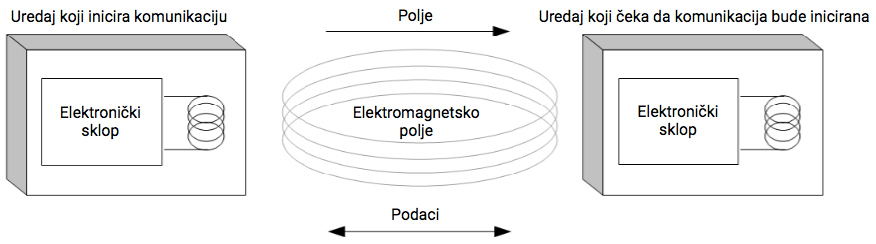
\includegraphics[height=4cm,keepaspectratio=true]{nfc_diagram}
 \caption{Komunikacija dva NFC ure\dj aja}
 \label{fig:nfc_arhitektura}
	\end{center}
\end{figure}

NFC ure\dj aji implementiraju dvije specifikacije i njihova funkcionalnost ovisi o tome po kojoj specifikaciji su izra\dj eni:

\begin{itemize}
	\item ISO/IEC 14443
	\begin{itemize}
		\item Definira memoriju NFC ure\dj aja
		\item Ure\dj aj je napravljen samo po ovoj specifikaciji je pasivni ure\dj aj i on ne mo\v{z}e inicirati komunikaciju (npr. naljepnica)
		
	\end{itemize}
	\item ISO/IEC 18092-3
	
	\begin{itemize}
		\item Definira elektromagnetsku komunikaciju (modulacije, kodiranje, inicijalizaciju...)
		\item Ovi ure\dj aji implementiraju i ISO/IEC 14443 specifikaciju i oni su aktivni ure\dj aji
	\end{itemize}
\end{itemize}

Nadalje, ovisno o vrstama NFC ure\dj aja koji komuniciraju, komunikacija se dijeli na pasivnu i na aktivnu.


\subsection{Aktivna komunikacija}

Aktivna NFC komunikacija ozna\v{c}ava dvosmjernu komunikaciju izme\dj u dva NFC ure\dj aja koji imaju vlastite izvore napajanja i izra\dj eni su po specifikaciji ISO/IEC 18092-3. Komunikacija se vr\v{s}i tako da ure\dj aj koji \v{z}eli poslati poruku aktivira svoje magnetsko polje preko kojega se poruka po\v{s}alje te ga deaktivira kada \v{z}eli primiti poruku. Ovakva komunikacija zahtjeva dodatnu logiku koja definira pravila komunikacije.

Aktivni NFC ure\dj aji se po arhitekturi dijele na \cite{nfc_types}:

\begin{itemize}
	\item NFC-A ure\dj aje
	\begin{itemize}
		\item Millerovo enkodiranje
		\item ASK modulacija 100%
		\item Brzina prijenosa 106 kb/s
	\end{itemize}

	\item NFC-B ure\dj aje
	\begin{itemize}
		\item Manchester enkodiranje
		\item ASK modulacija 10%
		\item Brzina prijenosa 106 kb/s
	\end{itemize}

	\item NFC-F (FeliCa) ure\dj aje
	\begin{itemize}
		\item Vrsta RFID protokola koja je jako sli\v{c}na NFC-u te stoga pripada istoj kategoriji
		\item Razvijena je u Japanu gdje ima jako \v{s}iroku primjenu (najra\v{s}irenija je kod prijevozni\v{c}kih karata)
		\item  Brzina prijenosa 212 kb/s
	\end{itemize}
\end{itemize}


\subsection{Pasivna komunikacija}

Pasivna komunikacija se vr\v{s}i izme\dj u aktivnog i pasivnog ure\dj aja, na na\v{c}in da aktivni ure\dj aj \v{s}alje signal nosioc kroz svoje elektromagnetsko polje \cite{nfc_arhitektura}. Ukoliko je pasivni ure\dj aj u dometu polje \'{c}e inducirati napon u njegovoj zavojnici te \'{c}e biti u stanju modulirati postoje\'{c}e polje, koriste\'{c}i ASK (amplitude-shift keying) modulaciju. To je znak aktivnom ure\dj aju da je komunikacija ostvarena. Nadalje, aktivni ure\dj aj provjerava koju vrstu komunikacije koristi pasivni ure\dj aj (npr. komunikacija mo\v{z}e biti enkriptirana - koristi se kod pla\'{c}anja kreditnim karticama), te ovisno o vrsti \v{s}alje odgovaraju\'{c}e zahtjeve za \v{c}itanjem memorije, \v{s}to mu pasivni omogu\'{c}ava nakon uspje\v{s}ne validacije.



Tipovi pasivnih NFC ure\dj aja uklju\v{c}uju \cite{nfc_pasivni}:

\begin{itemize}
	\item Tip 1
	\begin{itemize}
		\item Brisanje i \v{c}itanje memorije
		\item Mogu se konfigurirati samo za \v{c}itanje (read-only)
		\item Memorija: 96 B do 2kB
	\end{itemize}

	\item Tip 2
	\begin{itemize}
		\item Brisanje i \v{c}itanje memorije
		\item Mogu se konfigurirati samo za \v{c}itanje (read-only)
		\item Memorija: 48 B do 2kB
	\end{itemize}

	\item Tip 3
	\begin{itemize}
		\item Mogu ih \v{c}itati samo NFC-F ure\dj aji
		\item Ili konfigurabilni (\v{c}itanje i pisanje) ili samo za \v{c}itanje
		\item  Memorija varijabilna, teoretski mo\v{z}e biti do 1MB
	\end{itemize}

	\item Tip 4
	\begin{itemize}
		\item Ili konfigurabilni (\v{c}itanje i pisanje) ili samo za \v{c}itanje
		\item Memorija do 32 KB
	\end{itemize}
\end{itemize}


\section{Primjena}

Razvoj dana\v{s}nje tehnologije pru\v{z}a \v{c}ovje\v{c}anstvu sve opremljenije i prenosivije svakodnevne ure\dj aje. Samim time se pojavila potreba za protokolom \v{c}ija \'{c}e primjena biti \v{s}to br\v{z}e i jednostavnije  prenijeti informacije s ure\dj aja na ure\dj aj u kratkom dometu. Niska cijena, mogu\'{c}nost rada bez izvora energije i intinuitivnost kori\v{s}tenja (potrebno je samo prisloniti jedan NFC ure\dj aj na drugi) omogu\'{c}ava \v{s}iroku primjenu NFC-a, a neke od njih uklju\v{c}uju:

\begin{itemize}
	\item Beskontaktno pla\'{c}anje kreditnim karticama ili pametnim telefonima
	\item Otklju\v{c}avanje raznih ure\dj aja (ra\v{c}unala, automobila, brava...)
	\item Razmjena vizitki
	\item \v{c}itanje konfiguracije WiFi mre\v{z}e
	\item Otvaranje internetskih poveznica
	\item Ulaznice za razne doga\dj aje
\end{itemize}

Za potrebe ovog projekta kori\v{s}tene su NFC naljepnice kupljene preko internetske trgovine WhizTags \cite{whiztags}, prikazane na slici  ~\ref{fig:whiztags}.

\begin{figure}[!htbp]
	\begin{center}
 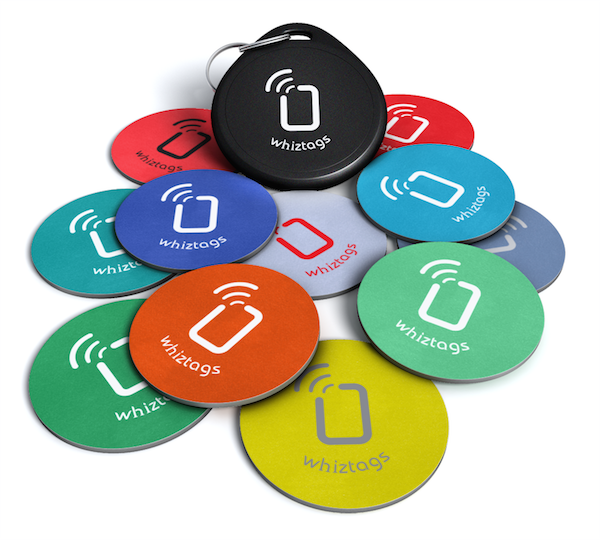
\includegraphics[height=8cm,keepaspectratio=true]{NTAG2161}
 \caption{Kori\v{s}tene NFC naljepnice}
 \label{fig:whiztags}
	\end{center}
\end{figure}

Specifikacija naljepnice:

\begin{itemize}
	\item NATG 216 NFC modul \cite{nat_modul}
	\item 888 B memorije
	\item Samoljepivost
	\item Vodootpornost
\end{itemize} 
\chapter{BLE tehnologija}
Bluetooth Low Energy (BLE ili Bluetooth Smart) je be\v{z}i\v{c}ni protokol koji uz pomo\'{c} radiovalova omogu\'{c}uje komunikaciju dva ili vi\v{s}e ure\dj aja. Protokol je prvotno je razvijan od kompanije Nokia pod imenom Wibree, ali 2007. godine dolazi pod jurisdikciju neprofitnog tijela Bluetooth Special Interest Group (SIG) \cite{sig}. SIG je organizacija koja nadgleda razvoj Bluetooth tehnologije i osigurava standardizaciju Bluetooth kompatibilnih ure\dj aja. 2010. godine BLE postaje nova iteracija Bluetooth protokola (verzija 4.0.) iako je u po\v{c}etku bio zami\v{s}ljen kao komplementarni protokol. Aktualna verzija specifikacije je 4.2 \cite{ble_specification}. Na na slici ~\ref{fig:ble} je prikazan logo BLE-a.

\begin{figure}[!htbp]
	\begin{center}
 
\includegraphics[height=3cm,keepaspectratio=true]{ble_logo}
 \caption{Logo BLE protokola}
 \label{fig:ble}
	\end{center}
\end{figure}

Glavna ideja BLE protokola je pru\v{z}iti funkcionanost Bluetooth-a uz \v{s}to manju potro\v{s}nju energije sa ure\dj ajima koji su manji, jeftiniji i optimiziraniji. U mobilnoj industriji Bluetooth protokol je ve\'{c} godinama standard te ga ve\'{c}ina ure\dj aja podr\v{z}ava i korisnici ga koriste koriste u ve\'{c} standradnim primjenama (povezivanje mobitela sa be\v{z}i\v{c}nom slu\v{s}alicom, uparivanje sa automobilom, prijenos podataka izme\dj u ure\dj aja). Me\dj utim, dolaskom BLE-a se podru\v{c}je primjene Bluetooth-a drasti\v{c}no pove\'{c}ava iz razloga \v{s}to je implementacija protokola puno dostupnija zbog slijede\'{c}ih razloga:

\begin{itemize}
	\item Danas gotovo svaki novi pametni telefon na tr\v{z}i\v{s}tu ima BLE \v{c}ip i time je tehnologija dostupa potencijalno ogromnom tr\v{z}i\v{s}tu
	\item \v{C}ipovi su jeftiniji, manji i zahtjevaju manje energije, \v{s}to otvara vrata mnogim novim implementacijama elektroni\v{c}kih ure\dj aja
	\item Protokol je za odre\dj ene primjene br\v{z}i jer za razliku od klasi\v{c}nog Bluetooth-a ne zahtjeva autentikaciju ure\dj aja
\end{itemize}


BLE tehnologiju treba gledati kao pro�irenje funkcionalnosti klasi\v{c}nog Bluetootha koji je primarno fokusiran na kontinuiranu razmjenu podataka relativno velikom brzinom, dok je BLE fokusiran na manju potro\v{s}nju energije pri komunikaciji. Manja potro\v{s}nja energije rezultira i ve\'{c}im brojem paralelnih konekcija (klasi\v{c}ni Bluetooth mo�e imati do 7 paralelnih konekcija, a BLE teoretski beskona\v{c}no). Danas obe iteracije Bluetooth specifikacije mogu koegzistirati na tr�i�tu, upravo zbog razli\v{c}itih primjena.

BLE je temelj za iBeacon tehnologiju, koja pru\v{z}a gotovo identi\v{c}ne funkcionalnosti ali je razvijana od tvrtke Apple pa se shodno tome striktno koristi samo sa Apple-ovim ure\dj ajima.

\section{Arhitektura}

BLE komunikacija se zasniva na radio valovima, u rasponu od 2.4 - 2.2835 GHz, preko kojih se \v{s}alju podatci, podjeljeni na pakete. Frekventni spektar BLE-a je podjeljen na 40 kanala od 2 MHz, te se svaki paket \v{s}alje zasebno kroz kanal \cite{ble_introduction}. Paket se prije slanja modulira GFSK (Gaussian frequency shift modulation) modluacijom i zatim \v{s}alje kroz kanal, teoretski maksimalnom brzinom od 1 Mbit/s (u praksi je to \v{c}esto manje zbog ograni\v{c}enja protokola i komunikacije radio valovima). Potro\v{s}nja energije je dvostruko manja od klasi\v{c}nog Bluetooth-a i iznosi 15 mA pri maksimalnom optere\'{c}enju modula, te se stoga ure\dj aji mogu napajati sa dugmastim baterijama (na ~\ref{fig:ble_baterija} je prikazana baterija koja je napajala BLE ure\dj aj koji je kori\v{s}ten u ovome radu) \v{s}to prili\v{c}no pridonosi prenosivosti, veli\v{c}ini i povoljnosti BLE ure\dj aja.


\begin{figure}[!htbp]
	\begin{center}
 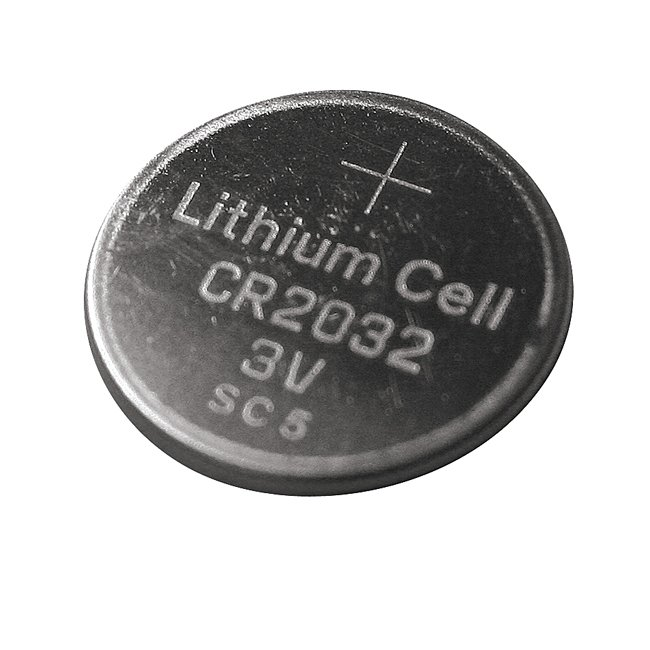
\includegraphics[height=4cm,keepaspectratio=true]{dugmasta_baterija}
 \caption{Dugmasta baterija koja pokre\'{c}e BLE ure\dj aja}
 \label{fig:ble_baterija}
	\end{center}
\end{figure}

Domet protokola u teoriji iznosi \v{c}ak do 100 metara u idealnim uvjetima, no u praksi je to do 10 metara. U praksi je manji domet zbog radio komunikacije, odnosno na oda\v{s}iljani radio signal mogu utjecati razne interferencije (apsorpcija signala u medij kroz koji prolazi, drugi signali), te iz razloga \v{s}to se cilja na to da ure\dj aji tro\v{s}e \v{s}to manje energije u radu pa se koriste slabije baterije s kojima BLE ure\dj aj ipak ima dovoljno dalek domet za ve\'{c}inu primjena.


\section{Topologija mre\v{z}e}

BLE ure\dj aj mo\v{z}e komunicirati sa drugim ure\dj ajima preko dva na\v{c}ina rada: ogla\v{s}avanje i uparivanje \cite{ble_getting_started}.

\subsection{Ogla\v{s}avanje}

Kod ogla\v{s}avanja ure\dj aj periodi\v{c}ki oda\v{s}ilje signal kojeg detektiraju svi ure\dj ji u dometu. To je jednosmjerna komunikacija i u kojoj razlikujemo oda\v{s}ilja\v{c}a koji konstantno \v{s}alje pakete (uvijek se \v{s}alje standardni paket od 31 B u kojem su osnovne informacije o ure\dj aju, a mogu\'{c}e je slati i dodatni paket sa dodatnim informacijama) i promatra\v{c}a koji konstantno skenira podru\v{c}je koje ga okru\v{z}uje. Ovaj na\v{c}in rada se koristi kada se \v{z}eli s jednim BLE ure\dj ajem slati ista informacija na vi\v{s}e ure\dj aja u dometu. Primjer ovakvog kori\v{s}tenja BLE protokola je proizvod ``Automatic museum guide'' od tvtke Locatify \cite{automatic_museum_guide} . Proizvod uklju\v{c}uje:


\begin{itemize}
	\item Ogla\v{s}iva\v{c}e (BLE ure\dj aje sa baterijom veli\v{c}ine kovanice)
	\begin{itemize}
		\item Postavljaju se u blizini muzejskih eksponata
	\end{itemize}
	\item CMS-a (Content management system)
	\begin{itemize}
		\item Sustav preko kojeg kustosi postavljaju sadr\v{z}aj o eksponatu u audio, video i tekstualnom obliku
	\end{itemize}
	
	\item Personaliziranu mobilnu aplikaciju
	\begin{itemize}
		\item Koriste\'{c}i BLE modul pametnog telefona konstantno skenira prostor i tra\v{z}i ogla\v{s}iva\v{c}e
	\end{itemize}
\end{itemize}

Svrha prozivoda je ta da korisnik sa upaljenom mobilnom aplikacijom dobiva preko pametnog telefona odre\dj eni sadr\v{z}aj kada u\dj e u domet ogla\v{s}iva\'{c}a. To se posti\v{z}e tako da mobilna aplikacija parsira ogla\v{s}iva\v{c}ev paket sa dodatnim podacima i na temelju dobivenih informacija preko CMS-a dobiva odgovaraju\'{c}i sadr\v{z}aj za specifi\v{c}an eksponat.
Prednosti ovakvog ogla\v{s}avanja su brzina i jednostavnost prijenosa, a mana je sigurnost, iz razloga \v{s}to odaslane pakete mogu primiti i ure\dj aji u dometu kojima ti paketi nisu namjenjeni.


\subsection{Uparivanje}
Uparivanje se koristi kod potrebe za sigurnom vezom izme\dj u dva ure\dj aja zbog dvosmjerne komunikacije. Kod komunikacije razlikujemo dvije vrste ure\dj aja:


\begin{itemize}
	\item Centralni ure\dj aj
	\begin{itemize}
		\item Skenira prostor i tra\v{z}i ure\dj aje s kojima mo\v{z}e komunicirati, te kada ih na\dj e inicira komunikaciju
		\item Odre\dj uje pravila komunikacije
	\end{itemize}
	\item Peripetalni ure\dj aj
	\begin{itemize}
		\item Oda\v{s}ilje ogla\v{s}iva\v{c}ke pakete kojima javlja ure\dj ajima u blizini da je spreman za komunikaciju
	\end{itemize}
\end{itemize}

Kada je komunikacija inicirana peripetalni ure\dj aj prestaje oda\v{s}iljati ogla\v{s}iva\v{c}ke pakete i komunicira samo sa centralnim ure\dj ajem. Obi\v{c}ajeni primjer ovakve komunikacije je komunikacija izme\dj u pametnog telefona i ure\dj aja sa nekim senzorom. Jedan od brojnih primjera je proizvod Rhythm+ od tvrtke Scosche \cite{scosche} . Radi se o pametnoj narukvici koja mjeri korisnikov puls te izmjerene podatke \v{s}alje centralnom ure\dj aju (pametnom telefonu sa kompatibilnom aplikacijom koja koristi dobivene podatke za kreiranje svoga sadr\v{z}aja).

Prednost uparivanja, kao na\v{c}ina rada BLE protokola, je sigurnost i optimizacija komunikacije. Ovaj na\v{c}in komunikacije je siguran jer se ure\dj aji moraju prepoznati i upariti da bi uop\'{c}e i moglo do\'{c}i do komunikacije, a optimizacija se posti\v{z}e jer centralni ure\dj aj odre\dj uje pravila komunikacije (koli\v{c}ina podataka koja se \v{s}alje, vremenski intervali u kojima se slanja odvijaju) i samim time se pove\'{c}ava propusnost podataka. Tako\dj er, osigurava se i malena potro\v{s}nja energije jer upareni ure\dj aji \v{s}alju podatke samo kada moraju, za razliku od na\v{c}ina rada gdje se paketi konstantno emitiraju.


\section{Primjena}
Primjena BLE ure\dj aja se temelji na profilu ure\dj aja koji je specificiran od strane SIG-a. Profili su uvedeni s namjerom da BLE ure\dj aji proizvedeni od razli\v{c}itih proizvo\dj a\v{c}a budu standardizirani i me\dj usobno kompatibilni. Tako\dj er, profili garantiraju da ure\dj aj, ovisno o svojoj primjeni, koristi BLE protokol na optimiziran na\v{c}in. Postoje dva op\'{c}a profila koja definiraju osnovna svojstva protokola \cite{ble_getting_started}:

\begin{itemize}
	\item Generic Access Profile (GAP)
	\begin{itemize}
		\item Specificira komunikaciju na najni\v{z}oj razini (ogla\v{s}avanje paketa i skeniranje okoline s ciljem ostvarivanja sigurn konekcije te ostvarivanje i odr\v{z}avanje veze me\dj u ure\dj ajima)
		\item Obavezno ga implementiraju svi BLE ure\dj aji
	\end{itemize}
	\item Generic Attribute Profile (GATT)
	\begin{itemize}
		\item Oslanja se na GAP te na vi\v{s}oj razini definira modele paketa i mehanizme za otkrivanje ure\dj aja i samu komunikaciju
	\end{itemize}
\end{itemize}

Nadalje, SIG je u specifikaciji BLE-a pru\v{z}io i konfiguraciju GATT profila za razna podru\v{c}ja primjene, sve kako bi korisnicima olak\v{s}ali implementaciju protokola u svoje proizvode. Konfiguracija uklju\v{c}uje definiranje komunikacije i na\v{c}ina rada ure\dj aja, kako bi protokol bio \v{s}to optimiziraniji. Neki od najzanimljivijih profila uklju\v{c}uju \cite{ble_profiles}: 


\begin{itemize}
	\item Prona\dj i me profil (FMP)
	\begin{itemize}
		\item Omogu\'{c}uje ure\dj aju da detektira lokaciju drugog ure\dj aja
	\end{itemize}
	
	\item Profil neposredne blizine (PXP)
	\begin{itemize}
		\item Oslanja se na GAP te na vi\v{s}oj razini definira modele paketa i mehanizme za otkrivanje ure\dj aja i samu komunikaciju
	\end{itemize}
	
	\item Profil HID preko GATT-a (HOGP)
	\begin{itemize}
		\item Omogu\'{c}ava slanje HID (Human Interface Device) podataka preko BLE ure\dj aja
		\item Ovaj profil se naj\v{c}e\v{s}\'{c}e koristi za upravljanje tipkovnicama, mi\v{s}evima i daljinskim ure\dj ajima
	\end{itemize}
	
	\item Glukozni profil (GLP)
	\begin{itemize}
		\item Koristi se za mjerenje glukoze kod pacijenata
	\end{itemize}
	
	\item Profil krvnog tlaka (BLP)
	\begin{itemize}
		\item Koristi se za mjerenje krvnog tlaka
	\end{itemize}
	
	\item Profil otkucaja srca (HRP)
	\begin{itemize}
		\item Koristi se za mjerenje otkucaja srca
	\end{itemize}
	
	\item Profil biciklisti\v{c}ke brzine i ritma (CSCP)
	\begin{itemize}
		\item Omogu\'{c}ava pra\'{c}enje brzine i ritma biciklisti\v{c}ke vo\v{z}nje
	\end{itemize}
\end{itemize}

Po navedenim profilima je vidljivo da je primjena BLE-a \v{s}iroka te da se BLE koristi u zdravstvu, sportu i rekreaciji, raznim senzorima i ra\v{c}unalstvu op\'{c}enito.

Za potrebe ovog projekta kori\v{s}ten je Gimbal Proximity Beacon Series 10 BLE ure\dj aj, koji je konfiguriran da radi u PXP profilu. Kupljen je preko internetske trgovine Gimbal \cite{gimbal_beacon} i prikazan na slici ~\ref{fig:gimbal_oglasivac}.

\begin{figure}[!htbp]
	\begin{center}
 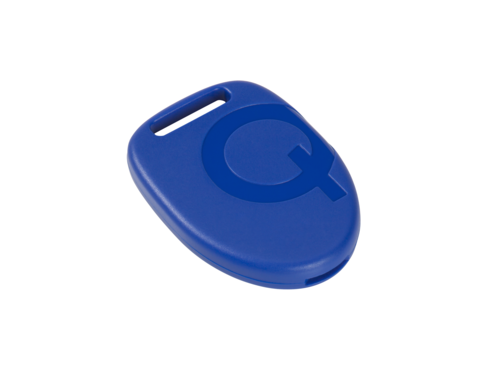
\includegraphics[height=7cm,keepaspectratio=true]{gimbal_s10}
 \caption{Komunikacija dva NFC ure\dj aja}
 \label{fig:gimbal_oglasivac}
	\end{center}
\end{figure}

Specifikacija ogla\v{s}iva\v{c}a:


\begin{itemize}
	\item Dimenzije: 40mm x 28 mm x 5.5 mm
	\item Temperaturni senzor
	\item Udaljenost prijenosa do 50 metara u idealnim uvjetima, u praksi do 10 metara
	\item CR2032 baterija za napajanje
	\item Kompatibilan sa iBeacon tehnologijom

\end{itemize}









   
\chapter{Izvedba}

Sustav kreiran kao prakti\v{c}ni dio ovoga rada se sastoji od mobilne i internetske aplikacije te je shodno tome ovo poglavlje podjeljeno na dva dijela u kojima su opisane korit\v{s}tene tehnologije i alati, te motivi za odabir istih. Iako su aplikacije iz razli\v{c}itih podru\v{c}ja ra\v{c}unarstva, razvoj im je organiziran i vo\dj en na isti nain, koriste\'{c}i alat Git \cite{git}. Git je alat kojeg je kreirao tim Linusa Torvaldsa (otac Linuxa i jedan od najbitnijih i zna\v{c}ajniji u ra\v{c}unarstvu uop\'{c}e) za potrebe razvoja jezgre Linux-a. Git slu\v{z}i za verzioniranje i organizaciju koda i funkcionira na na\v{c}in da korisnik grupira napravljene promjene u cjeline (commit-ove) koji \v{c}ine logi\v{c}ke cjeline (branch-eve) koje obi\v{c}no predstavljaju funkcionalnosti aplikacije. Na taj na\v{c}in je cijeli razvoj projekta evidentiran i u bilo kojem trenutku se mo\v{z}e vratiti na neko pro\v{s}lo stanje. Posebno je koristan u organizaciji timova od vi\v{s}e ljudi jer omogu\'{c}ava da vi\v{s}e ljudi radi na razl\v{c}iitim djelovima projketa (\v{c}ak i na istom kodu jer posjeduje mehanizam za rje\v{s}avanje konflikata nastalih ure\dj enjem iste linije koda od vi\v{s}e programera). U praksi se koriste i razli\v{c}ite metode kori\v{s}tenja Git-a, od kojih je naj\'{c}e\v{s}\'{c}e kori\v{s}tena ``Git flow'' \cite{git_flow}, koja specificira organizaciju branch-eva s ciljem standardizacije i efektivnijeg kori\v{s}tenja Git-a. Nadalje, u praksi se Git koristi u kombinaciji sa platformama za pohranjivanje projekata \v{s}to omogu\'{c}uje decentralizaciju projekta, kolaboraciju vi\v{s}e programera i sigurnost (rezervna kopija je serveru). Oba projekta koriste platformu Github \cite{github} koja je jedna od najkori\v{s}tenijih platformi za projekte otvorenog koda. Uz navedene prednosti, Github pru\v{z}a i dodatne statistike i informacije o projektu, kao npr. aktivnost graf napravljenih commitova u vremenu, prikazan na slici  ~\ref{fig:commits}.

\begin{figure}[!htbp]
	\begin{center}
 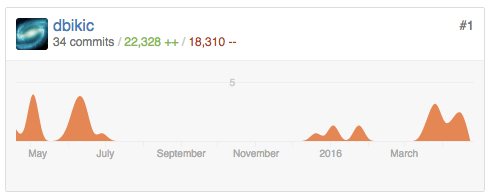
\includegraphics[height=4.2cm,keepaspectratio=true]{git_commits}
 \caption{Graf commit-ova u vremenskom periodu za projekt mobilne aplikacije}
 \label{fig:commits}
	\end{center}
\end{figure}

\section{Mobilna aplikacija}

\subsection{Tehnologija}
Klijenstska mobilna aplikacija je razvijena za Android operativni sustav, \v{c}iji je logo prikazan na slici ~\ref{fig:android}. Android je baziran na Linux jezgri te je kao takav projekt otvorenog otvorenog koda. Razoj Androida vodi tvrtka Google (2005. godine Google kupuje tvrtku Android Inc. koja je po\v{c}ela sa razvojem Android-a \cite{kupnjaAndroida}) koja u suradnji s proizvo\dj a\v{c}ima pametnih telefona kreira Android operativni sustav kojeg ure\dj aji na tr\v{z}i\v{s}tu imaju instaliranog. Takav Android nije u potpunosti otvorenog koda jer uklju\v{c}uje aplikacije koje nisu otvorenog koda (najva\v{z}nija je Google Play \cite{googlePlay}, centralna platforma za distibuciju aplikacija, glazbe i filmova).

\begin{figure}[!htbp]
	\begin{center}
 
\includegraphics[height=4cm,keepaspectratio=true]{android}
 \caption{Logo Android-a}
 \label{fig:android}
	\end{center}
\end{figure}

Zbog otvorenosti koda i mogu\'{c}nosti da svaki proizvo\dj a\v{c} kreira svoju verziju sustava (sa Google-ovim modulima ili bez), Android je danas najrasprostranjenija mobilna plaforma (danas svako drugo kupljeno ra\v{c}unalo ima instaliran Android operativni sustav \cite{androidDominacija}).

Aplikacije za Android platformu se razvijaju u Java programskom jeziku (iako danas postoje kvalitetne alternative, prvenstveno zbog zastarijelosti Jave, koja je razvijena po\v{c}etkom 1990. godine, npr. Kotlin \cite{kotlin}), na na\v{c}in da se jezgra Java-e pro\v{s}iri sa Android SDK-om (Software Developtment Kit - skup alata, biblioteka i dokumentacije koji skupa \v{c}ine platformu za razvoj Android aplikacija). 

Android aplikacije se na pametnom telefonu izvr\v{s}avaju na na\v{c}in da se za svaku aplikaciju u okru\v{z}ju za izvr\v{s}avanje kreira instanca virtualnog stroja. 
Virtualni stroj pokre\'{c}e aplikacije tako da pokrene .dex datoteke koje se dobivaju prevo\dj enjem bytecode datoteka aplikacije (bytecode datoteke nastaju prevo\dj enjem izvornih .java datoteka i to radi okru\v{z}je za razvoj Android aplikacija). Do Android verzije 5.0 se za okru\v{z}je za izvr\v{s}avanje koristilo Dalvik VM okru\v{z}je, koje je kod svakog pokretanja aplikacije prevodio bytecode u .dex datoteke. Od Android 5.0 se koristi ART okru\v{z}enje koje vr\v{s}i prevo\dj enje bytecode datoteka unaprijed, odnosno prilikom instalacije aplikacije. Na taj na\v{c}in se smanjuje broj prevo\dj enja \v{s}to rezultira smanjivanjem kori\v{s}tenja procesora ure\dj aja i smanjenjem potro\v{s}nje baterije \cite{dalvikArt}.



\subsection{Alati}
Android studio
http://developer.android.com/tools/studio/index.html

Razvoj Android aplikacija se vr\v{s}i u integriranom razvojnom okru\v{z}enju Android Studio \cite{androidStudio}. Baziran je na okru\v{z}enju IntelliJ IDEA \cite{inteliJ} tvrtke JetBrains (ista tvrtka koja razvija programski jezik Kotlin \cite{kotlin}). Programerima pru\v{z}a razne funkcionalnosti koje uklju\v{c}uju:

\begin{itemize}
		\item Sustav izgradnje baziran na sustavu Gradle \cite{gradle}
		\begin{itemize}
			\item Pru\v{z}a jednostavno verzioniranje aplikacija, dodavanje knji\v{z}ica, testiranje aplikacije
		\end{itemize}
		\item Omogu\'{c}avanja izgradnje razli\v{c}itih verzija iste aplikacije
		\begin{itemize}
			\item Korisno ako programer \v{z}eli napraviti besplatu i pla\'{c}enu verziju aplikacije ili imati verziju aplikacije za testno i produkcijsko okru\v{z}enje
		\end{itemize}
		\item Intuitivni ure\dj iva\v{c} korisni\v{c}kih su\v{c}elja
	\end{itemize}


\section{Internetska aplikacija}

\subsection{Tehnologije}

Internetska aplikacija se sastoji od dva dijela: klijentskog i poslu\v{z}iteljskog. Iako se oba dijela nalaze na istom poslu\v{z}itelju, razlika izme\dj u njih je u lokaciji na kojoj se kod izvr\v{s}ava. Klijentski dio se izvr\v{s}ava u korisni\v{c}kom pregledniku te on uklju\v{c}uje korisni\v{c}ko su\v{c}elje aplikacije, dok se poslu\v{z}iteljski dio izvr\v{s}ava na poslu\v{z}itelju te on uklju\v{c}uje bazu podataka, su\v{c}elje za pristupanje istoj.

Korisni\v{c}ko su\v{c}elje je kreirano uz pomo\'{c} tri standardne internetske tehnologije koje su temelj interneta kakav je danas: HTML, CSS i Javascript. HTML \cite{html} (Hyper Text Markup Language) je standardni jezik za kreaciju elemenata internetske stranice i temelj za sav daljnji dizajn i logiku. CSS \cite{css} (Cascading Style Sheets) slu\v{z}i za definiranje stilova koji se dodaju HTML elementima i koje preglednik interpretira te na temelju njih definira izgled, poziciju i pona\v{s}anje elemenata. Javascript \cite{javascript} se koristi za interakciju korisnika i internetske stranice, te za manipulaciju HTML elemenata.

Poslu\v{z}iteljska strana uklju\v{c}uje MySQL bazu podataka i PHP skripte koje dohva\'{c}aju podatke iz iste te ih u obliku HTML elemenata prikazuju na korisni\v{c}kom su\v{c}elju. MySQL je sustav za upravljanje bazama podataka koji uklju\v{c}uje relacijsku bazu podataka kojojm se upravlja pomo\'{c}u SQL (Structured Querry Language) jezika. PHP (Hypertetxt Preprocessor) je skriptni jezik koji se koristi na poslu\v{z}iteljskoj strani za komunikaciju sa bazom. Funkcionira tako da se u HTML kod ugra\dj uje skriptni kod kojeg poslu\v{z}itelj prepoznaje i izvr\v{s}ava, te se rezultat izvr\v{s}avanja ispisuje u HTML kod koji se onda \v{s}alje klijentu.

Opisane tehnologije su izabrane prvenstveno zato jer su sve otvorenog koda, a zatim jer su standard u domeni internetskih aplikacija (HTML, CSS, Javascript) i jer im je primjena ra\v{s}irena i \v{c}esto se koriste u praksi (MySQL, PHP).

\subsection{Alati}
Kori\v{s}teni alati za izradu internetske aplikacije su:
\begin{itemize}
	\item Atom 1.6.2 \cite{atom}
	\begin{itemize}
		\item Ure\dj iva\v{c} koda razvijen od tvrtke GitHub
		\item Kori\v{s}ten za pisanje svog koda (HTML, CSS, Javascript i PHP)
	\end{itemize}
	
	\item XAMPP 5.6.12-0 \cite{xampp}
	\begin{itemize}
		\item Paket alata namjenjen za poslu\v{z}itelje koji uklju\v{c}uje HTTP poslu\v{z}itelj, MySQL bazu podataka i interpreter programskih jezika PHP i Pearl
		\item Kori\v{s}ten je za kreiranje lokalnog testnog poslu\v{z}itelja i za kreiranje i administraciju baze podataka pomo\'{c}u alata phpMyAdmin
	\end{itemize}
	
	\item FileZilla 3.16.1 \cite{filezilla}
	\begin{itemize}
		\item Klijent za SFTP (Secure File Transfer Protocol) prijenos datoteka na poslu\v{z}itelj
	\end{itemize}
\end{itemize}



\chapter{Android aplikacija}

\section{Arhitektura}

Napravljena Android aplikacija ima slijede\'{c}e uvijete za ure\dj aje na kojima se mo\v{z}e pokrenuti:

\begin{itemize}
		\item Minimalna verzija Android operativnog sustava je 5.0. (Android SDK verzija 21, kodnog naziva Lollipop)
		\item NFC modul
		\item BLE modul
\end{itemize}

\subsection{MVP}

Aplikacija je implementirana slijede\'{c}i MVP oblikovni obrasac \cite{mvp}. Svrha ovog obrasca je logi\v{c}ki strukturirati aplikaciju na na\v{c}in da se prezentacijski sloj odvoji od poslovne logike aplikacije. Prezentacijski sloj uklju\v{c}uje korisni\v{c}ko su\v{c}elje i sve \v{s}to korisnik vidi, \v{c}uje ili osjeti pomo\'{c}u pametnog telefona, dok poslovna logika uklju\v{c}uje dohva\'{c}anje i obradu podataka koji se prikazuju na su\v{c}elju te op\'{c}enito svu logiku koju aplikacija implementira. Razlog uvo\dj enja slojeva i odvajanja logike od prezentacijskog dijela je kreacija odr\v{z}ivog sustava kojeg je jednostavno nadograditi i testirati. Prednost je i to \v{s}to je kod strukturiran i \v{c}itljiv, \v{s}to olak\v{s}ava rad vi\v{s}e ljudi na istom projektu i odr\v{z}avanje istog.

Na slici ~\ref{fig:mvp} je prikazana shema komunikacije izme\dj u slojeva u MVP oblikovnom obrascu.

\begin{figure}[!htbp]
	\begin{center}
 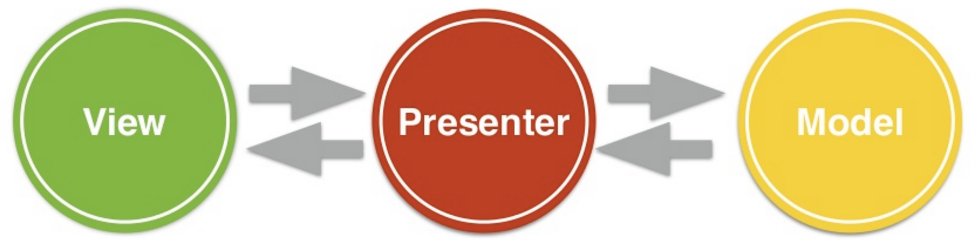
\includegraphics[height=3.5cm,keepaspectratio=true]{mvp}
 \caption{Komunikacija slojeva u MVP oblikovnom obrascu}
 \label{fig:mvp}
	\end{center}
\end{figure}

Sloj View je jedini sloj s kojim korisnik ima direktnu interakciju. On ima za zada\'{c}u prikazati podatke na korisni\v{c}kom su\v{c}elju i reagirati na sve korisni\v{c}ke interakcije (npr. odabir elementa liste, dodir gumb...). View u sebi posjeduje referencu na Presenter i njegova uloga je zapravo pozivati odgovaraju\'{c}e metode Presentera nakon \v{s}to se dogodi odre\dj ena akcija i prikazivanje podataka koje mu Presenter proslijedi.

Sloj Presenter sadr\v{z}i glavnu logiku Android aplikacije iz razloga \v{s}to je posrednik izme\dj u View i Model sloja. On odlu\v{c}uje kako reagirati na neku korisnikovu akciju, na koji na\v{c}in dohvatiti podatke iz Model sloja i op\'{c}enito odre\dj uje cijelo korisni\v{c}ko iskustvo sa aplikacijom.

Sloj Model je zadu\v{z}en za dohva\'{c}anje podataka (iz interne memorije ure\dj aja, baze podataka aplikacije ili internetskog poslu\v{z}itelja) i serijaliziranje istih u modele koji se koriste u ostatku aplikacije. Iz tog razloga se dijeli na dva dijela: interactor (vr\v{s}i interakciju sa podacima) i same modele (Java klase).

MVP se na Android platformi, u programskom jeziku Java, implementira uz pomo\'{c} su\v{c}elja u kojima su definirani prototipi metoda koje klasa koja implementira su\v{c}elje mora implementirati. Ovaj na\v{c}in podi\v{z}e razinu apstraktnosti i dopu\v{s}ta programeru da prvo dobro logi\v{c}ki osmisli najbolji na\v{c}in za napraviti MVP sa datim zahtjevima, s ciljem maksimiziranja efekata obrasca, a zatim da se posveti i samoj implementaciji. Na slici ~\ref{fig:mvp} je na primjeru dohva\'{c}anja konfiguracije poslovnice prikazana implementacija MVP obrasca u napravljenoj Android aplikaciji.


\begin{figure}[!htbp]
	\begin{center}
 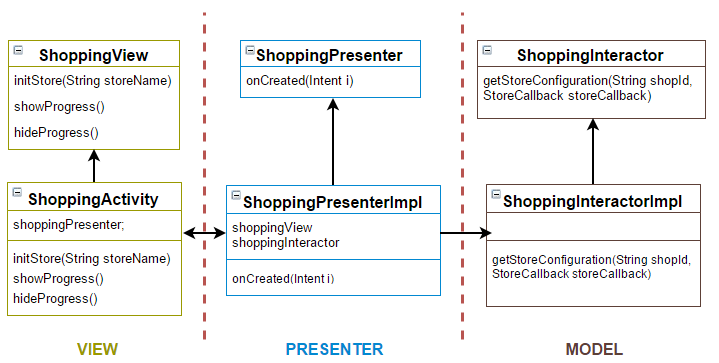
\includegraphics[height=7.5cm,keepaspectratio=true]{mvp_primjer}
 \caption{Primjer MVP-a u napravljenoj aplikaciji}
 \label{fig:mvp}
	\end{center}
\end{figure}

Slika ~\ref{fig:mvp} prikazuje tijek doga\dj aja od trenutka kada korisnik skenira NFC tag do trenutka kada mu se prikazuje su\v{c}elje za poslovnicu u kojoj se nalazi. Klasa ShoppingActivity je Java klasa koja pro\v{s}iruje klasu Activity (aktivnost), koja dolazi sa Android SDK-om. Aktivnost je najlak\v{s}e tuma\v{c}iti kao jedan zaslon aplikacije, te ShoppingActivity predstavlja zaslon koji je korisniku predstavljen u trenutku kada se on nalazi u poslovnici te je u potrazi za popustima.

U trenutku kada korisnik skenira NFC naljepnicu pokre\'{c}e se aktivnost ShoppingActivity (u potpoglavlju 3.1.2 ``Pasivna komunikacija'' je detaljno opisan mehanizam koji ovo omogu\'{c}uje). Ona implementira ShopingView su\v{c}elje i ima referencu na ShoppingPresenterImpl objekt koji implementira ShoppingPresenter, kojemu zove metodu onCreated(Intent i). ShoppingPresenterImpl tada iz objekta Intent i \v{c}ita identifikacijski broj poslovnice te je spreman inicirati zahtjev za dohva\'{c}anje podataka o poslovnici sa poslu\v{z}itelja. Prvo zove metodu showProgress() (implementirana u aktivnosti ShoppingActivity) koja slu\v{z}i da bi korisniku prikazao ProgressDialog (mehanizam koji korisniku prikazuje indikator da pri\v{c}eka jer se neka operacija izvr\v{s}ava, prikazan je na slici ~\ref{fig:progressDialog}), te zatim zove metodu interaktorovu metodu getStoreConfiguration() (implementiranu u klasi ShoppingInteractor) kojoj predaje identifikaciju poslovnice i objekt koji implementira su\v{c}elje StoreCallback.


\begin{figure}[!htbp]
	\begin{center}
 
\includegraphics[height=3cm,keepaspectratio=true]{progressDialog}
 \caption{ProgressDialog koji korisniku daje do znanja da mora pri\v{c}ekati jer se neka operacija obavlja u pozadini}
 \label{fig:progressDialog}
	\end{center}
\end{figure}

Metoda getStoreConfiguration() kreira zahtjev za konfiguracijom poslovnice poslu\v{z}itelju. Praksa je da se zahtjev izvr\v{s}ava na novoj dretvi iz razloga \v{s}to se vrijeme potrebno poslu\v{z}itelju za odgovor ne mo\v{z}e unprijed znati, te nema smisla da glavna dretva aplikacije zbog toga bude blokirana (to rezultira zamrznutim ekranom telefona \v{s}to korisnike jako odbija od aplikacije). Zbog navedenog razloga, interaktoru se \v{s}alje objekt storeCallback koji implementira su\v{c}elje StoreCallback prikazano na slici ~\ref{fig:storeCallback}, koje definira metodu za uspjeh i neuspjeh zahtjeva. Ukoliko je zahtjev uspio, ineraktor serijalizira dobivene podatke u odgovaraju\'{c}i model (serijalizacija je potrebna jer poslu\v{z}itelj vra\'{c}a podatke u JSON formatu) kojega preko su\v{c}elja \v{s}alje nazad prezenteru. Ukoliko zahtjev nije uspio (npr. poslu\v{z}itelj nije aktivan ili telefon nema pristup internetu) zove se metoda za neuspjeh koja za krajnji cilj ima korisniku prikazati da je do\v{s}lo do gre\v{s}ke.


\begin{figure}[!htbp]
	\begin{center}
 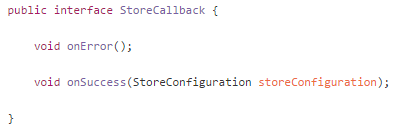
\includegraphics[height=3cm,keepaspectratio=true]{storeCallback}
 \caption{Su\v{c}elje StoreCallback sa prototipima metoda za uspjeh i neuspjeh zahtjeva za konfiguracijom poslovnice.}
 \label{fig:storeCallback}
	\end{center}
\end{figure}

Prvo \v{s}to prezenter napravi nakon \v{s}to dobije interaktorov odgovor je sakrivanje ProgressDialog-a na na\v{c}in da pozove metodu hideProgress() u aktivnosti. Nakon toga, inicijalizira su\v{c}elje sa informacijama o poslovnici te kao vlastiti atribut sprema listu popusta, koje evaluira nakon \v{s}to mu aktivnost javi da je BLE ogla\v{s}iva\v{c} prona\dj en, na isti na\v{c}in kao \v{s}to mu je javila da je korisnik u\v{s}ao u poslovnicu. Sva logika aplikacije je implementirana na istim principima MVP-a, \v{s}to ju \v{c}ini mnogo \v{c}itljivijom i bolje organiziranom od toga da je sve implementirano u klasi aktivnosti.

\subsection{NFC komunikacija}

Za potrebe ovog projekta je implementirana jendosmjerna NFC komunikacija izme\dj u pametnog telefona i NFC naljepnice. Zahtjev projekta uklju\v{c}uje pokretanje aktivnosti za tra\v{z}enje popusta prilikom skeniranja NFC nalijepnice u odre\dj enoj poslovnici. To je omuge\'{c}no pomo\'{c}u mehanizma u Android operativnom sustavu koji zapo\v{c}inje instalacijom aplikacije na pametni telefon. Prilikom instalacije Android analizira sadr\v{z}aj datoteke AndroidManifest \cite{androidManifest} u kojoj su specificirane najva\v{z}nije informacije o aplikaciji, koje me\dj u ostalim uklju\v{c}uju: ime paketa aplikacije, popis svih aktivnosti u aplikaciji, dozvole koje aplikacija zahtjeva (npr. NFC, BLE, kamera, mikrofon). Prilikom definiranja aktivnosti aplikacije, mogu\'{c}e je definirati da je odre\dj ena aktivnost sposobna obraditi odre\dj enu vrstu podataka. Ti podatci su su objekti klase Intent (eng. namjera, klasa definirana u Android SDK-u) te sadr\v{z}e opis akcije koja se treba izvr\v{s}iti i dodatne podatke. Kod instaliranja nove aplikacije, operativni sustav u svoju internu memoriju zapisuje aktivnosti koje su sposebne za obradu odre\dj ene vrste Intenta. Kada tokom kori\v{s}tenja telefona do\dj e do zahtjeva za Intentom, Android provjeri koje aplikacije mogu obraditi taj intent i korisniku prika\v{z}e izbornik u kojem odabire \v{z}eljenu aplikaciju (mo\v{z}e se definirati i predodre\dj ena aplikacija pa se izbornik ne\'{c}e prikazivati).

Ozna\v{c}avanje aktivnosti kao sposobne za obraditi Intent se radi pomo\'{c}u Intent filtera, u kojem se obavezno mora specificirati ime akcije. Na slici \ref{fig:intentFilter} je prikazan zapis iz AndroidManifet-a za aktivnost koja sadr\v{z}i logiku za \v{c}itanje NFC nalijepnica namjenjenih za ovu aplikaciju, koja uklju\v{c}uje odgovaraju\'{c}i Intent filter.

\begin{figure}[!htbp]
	\begin{center}
 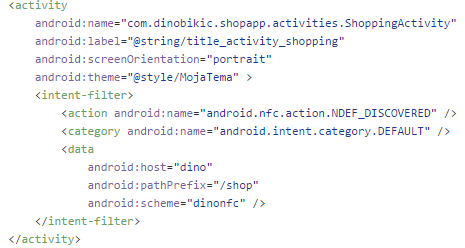
\includegraphics[height=6cm,keepaspectratio=true]{intentFilter}
 \caption{Primjer definiranja aktivnosti sa IntentFilter-om u AndroidManifest-u}
 \label{fig:intentFilter}
	\end{center}
\end{figure}

Kada korisnik uklju\v{c}i NFC modul na svome ure\dj aju, Android u pozadini skenira okolinu pomo\'{c}u NFC senzora te kada nai\dj e na NFC ure\dj aj kreira Intent objekt s akcijom koja ovisi o vrsti podacima zapisanim na NFC ure\dj aju. Za potrebe projekta, sve NFC naljepnice su morale imati u svojoj memoriji zapisan URI u kojem je specificirano ime paketa aplikacije koja obra\dj uje pro\v{c}itane podatke i identifikacija poslovnice. Takvi NFC ure\dj aji su prema NFC Forum-u specificirani kao NDEF \cite{NdefMessage} (Android naziva akciju nala\v{z}enja ovakvih ure\dj aja \verb|NDEF_DISCOVERED| \cite{ndef_discovered}).
Stoga, ovakva konfiguracija za rezultat ima pokretanje aktivnost ShoppingActivity pri skeniranju NFC naljepnice. ShoppingActivity tada \v{s}alje cijeli Intent objekt u prezenter koji \v{c}ita vrijednost skenirane naljepnice te radi zahtjev za konfiguracijom poslovnice u kojoj se korisnik nalazi.

\subsubsection{Priprema NFC naljepnice}
Za zapis podataka na naljepnicu je kori\v{s}tena aplikacija NFC Tools \cite{nfcTools}. Aplikacija ima pla\'{c}enu i besplatnu verziju, a za potrebe projekta je bila dovoljna besplatna verzija preko koje se sa naljepnice mogu \v{c}itati i zapisivati podaci. Proces zapisivanja URI-a je prikazan na slici \ref{fig:zapisNfca}.


\begin{figure}[!htbp]
	\begin{center}
 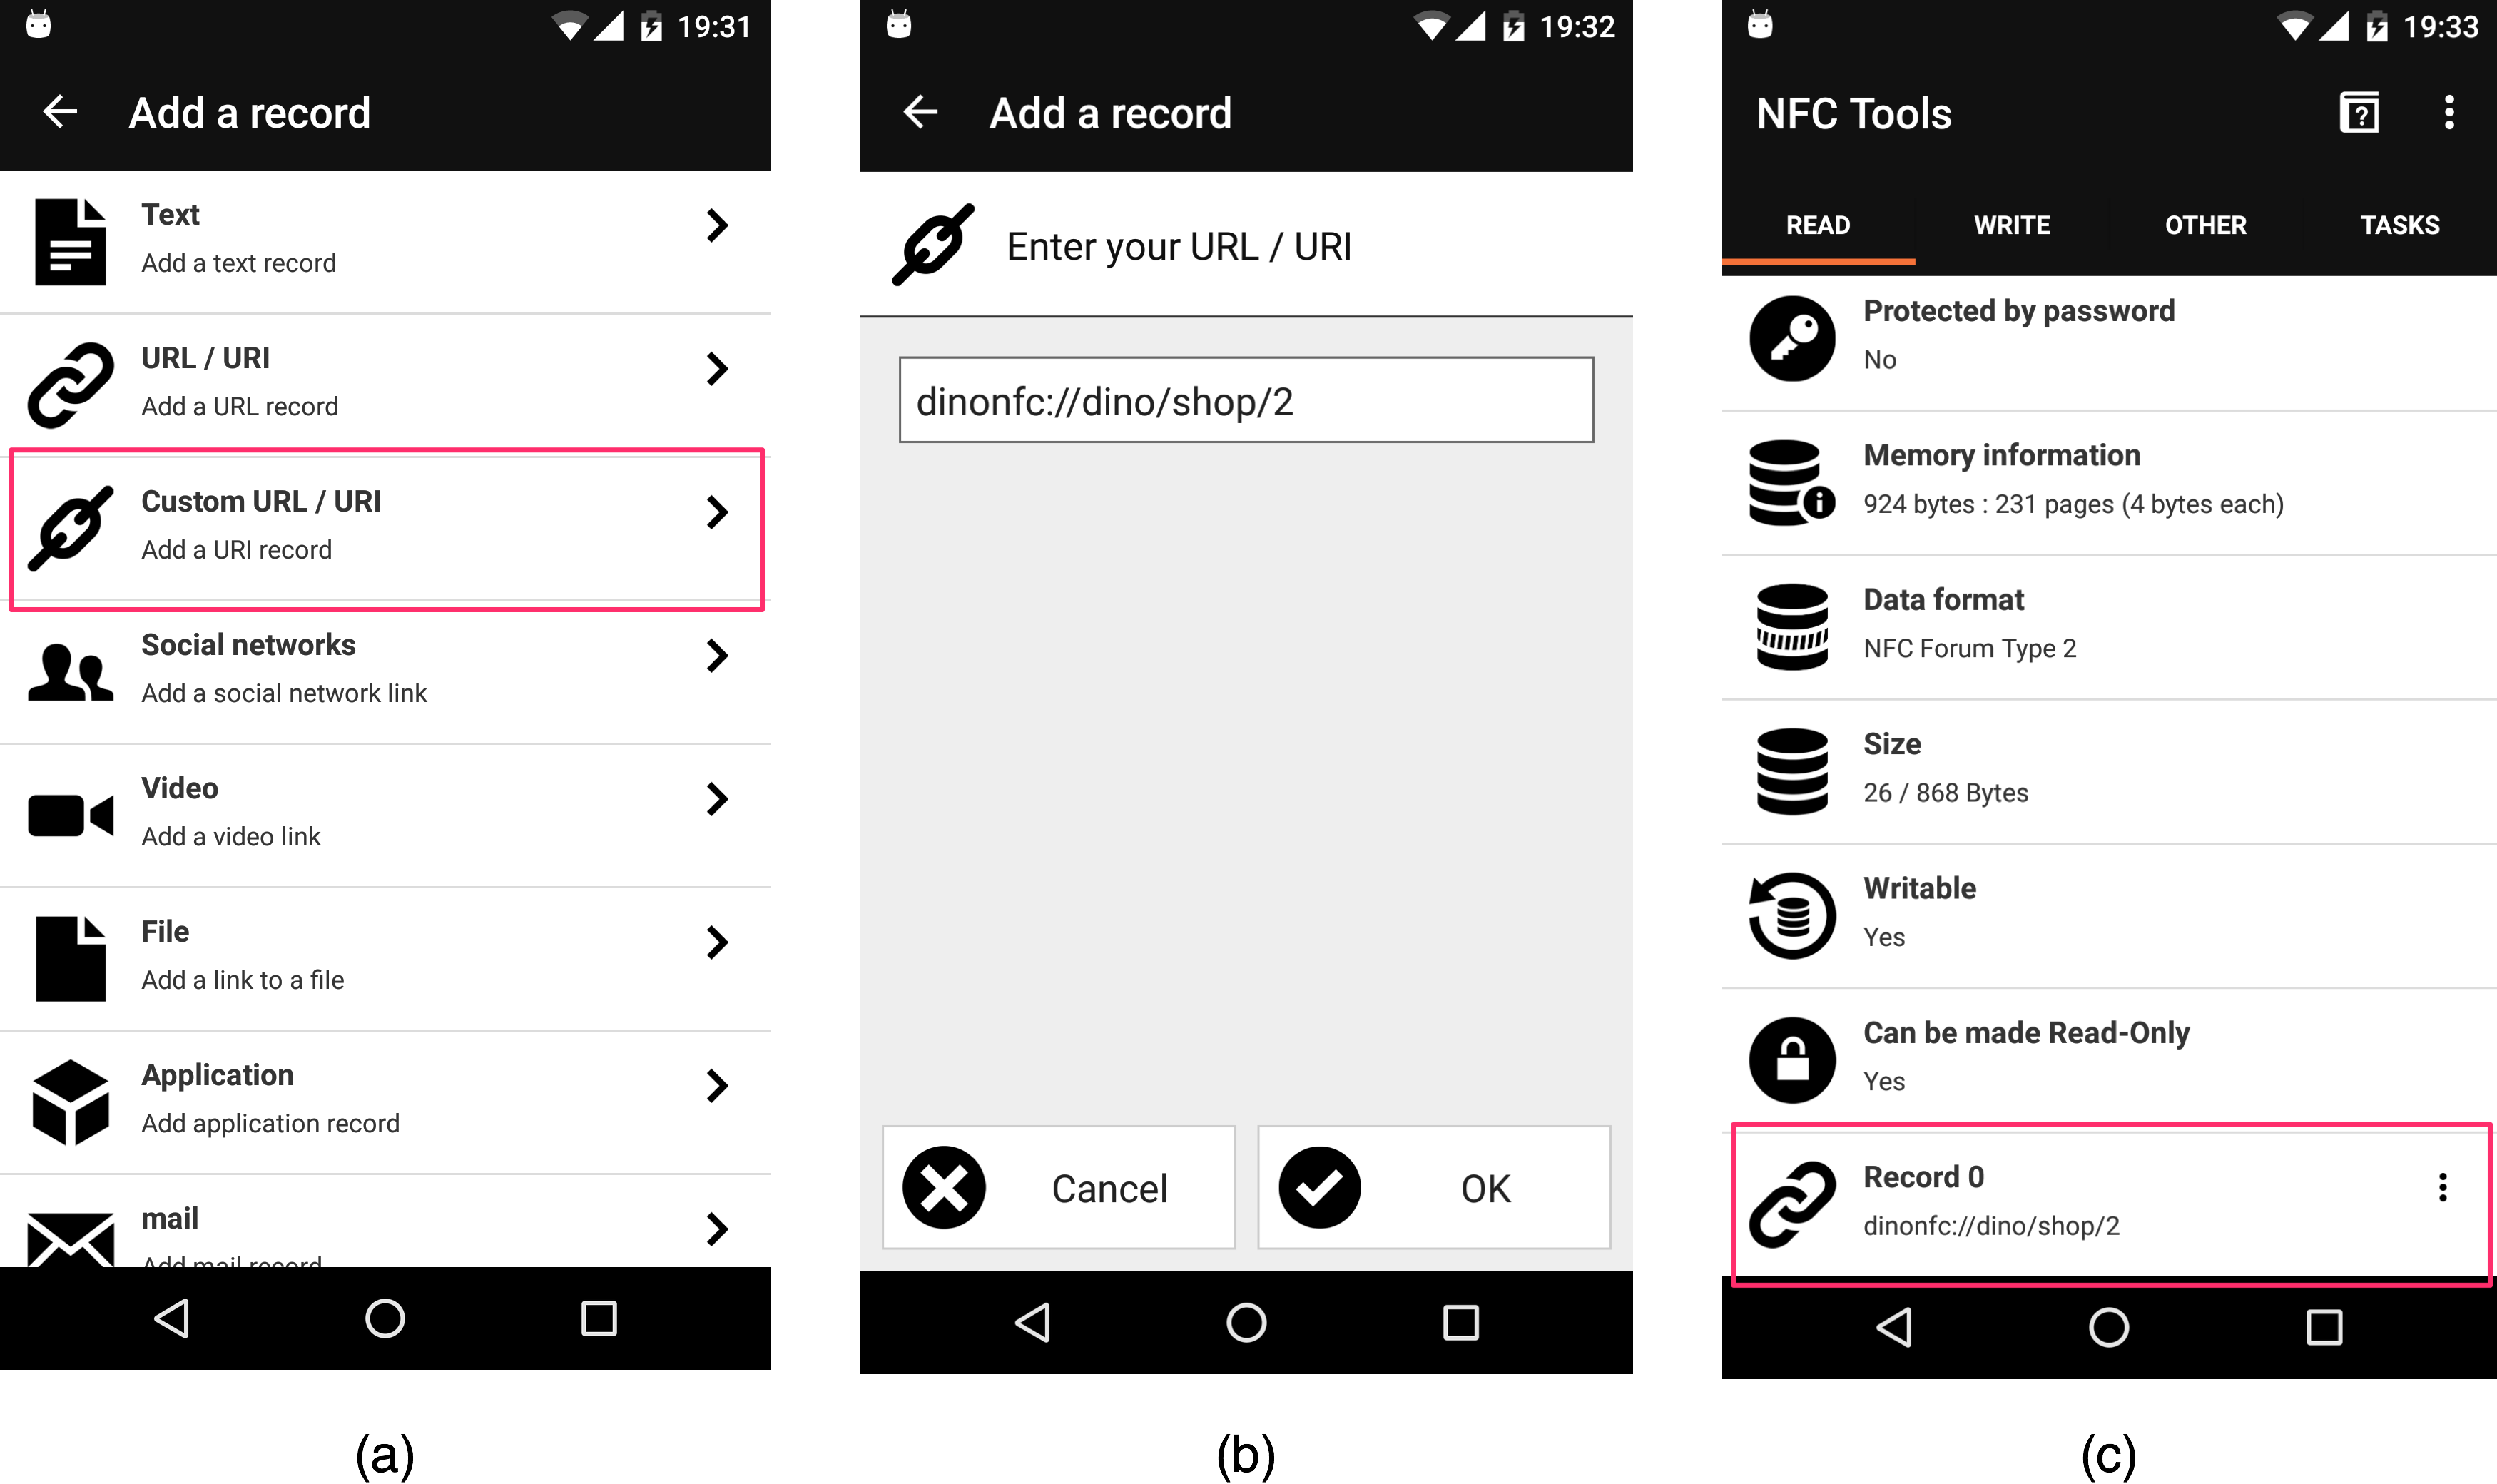
\includegraphics[height=9cm,keepaspectratio=true]{zapis_nfca}
 \caption{Na slici je prikazan proces zapisivanja URI-a na NFC nalijepnicu. Ekran (a) prikazuje odabir zapisivanja URI-a, ekran (b) prikazuje upisivanje URI-a. Nakon \v{s}to je URI upisan potrebno je prisloniti naljepnicu na pametni telefon, s ciljem zapisivanja podataka. Ekran (c) prikazuje pro\v{c}itani zapis nalijepnice kojoj smo prethodno zapisali URI.}
 \label{fig:zapisNfca}
	\end{center}
\end{figure}

Struktura URI-a je takva se prvo navodi shema, koja ozna\v{c}ava vrstu URI-a, zatim ime doma\'{c}ina i prefiks puta, te naposlijetku identifikator poslovnice. Ove informacije su potrebne da se kreira ispravan Intent objekt pomo\'{c}u kojeg \'{c}e Android operativni sustav otvoriti ispravnu aplikaciju koja \'{c}e ga obraditi.

\subsection{BLE komunikacija}

Prvi uvjet da se komunikacija izme\dj u pametnog telefona i ogla\v{s}iva\v{c}a mo\v{z}e ostvariti je da je ogla\v{s}iva\v{c} aktivan i da se nalazi u dometu telefona. Drugi uvjet je da pametni telefon ima instaliranu minumalnu verziju 5.0. Android operativnog sustava iz razloga \v{s}to je na Android platformi BLE komunikacija izme\dj u ure\dj aja i ogla\v{s}iva\v{c}a implementirana pomo\'{c}u klase BluetoothLeScanner \cite{bluetoothLeScaner} koja se nalazi u Android SDK-u (prisutna od verzije 21, odnosno Android verzije 5.0).
Objekt klase BluetoothLeScanner je zapravo \v{c}lan u objekta klase BluetoothAdapter \cite{bluetoothAdapter}, koja je zadu\v{z}ena za sve operacije sa Bluetooth modulom ure\dj aja. Ukoliko pametni telefon nema ugra\dj eni BLE modul, objekt klase BluetoothAdapter vrati vrijednost null za BluetoothLeScanner \v{s}to ozna\v{c}ava da skeniranje nije mogu\'{c}e. Ukoliko vrati ispravan objekt, skeniranje okoline je mogu\'{c}e i ono zapo\v{c}inje pozivanjem metode startScan(ScanCallback callback) od BluetoothLeScanner objekta. Objekt callback je implementacija su\v{c}elja ScanCallback. Kada smo ispravno zapo\v{c}eli skeniranje, Android sustav \'{c}e svaki put kada detektira BLE ure\dj aj pozvati metodu onScanResult(int callbackType, ScanResult result) ScanCallback objekta te predati objekt klase ScanResult. Klasa ScanResult sadr\v{z}i informacije o ja\v{c}ini detektiranog signala, vremenu detekcije i najva\v{z}nije, o detektiranom ure\dj aju. Informacije o detektiranom ure\dj aju uklju\v{c}uju njegovu strojnu adresu, vrstu BLE ure\dj aja i vrstu veze. Po\v{s}to je strojna adresa ure\dj aja jednozna\v{c}na i ne postoje dva ure\dj aja sa istom strojnom adresom, ona je kori\v{s}tena u aplikaciji za implementaciju funkcionalnosti, na na\v{c}in da je popust vezan za BLE ure\dj aj.


\section{Implementacija ekrana}

Aplikacija se sastoji od 4 glavna ekrana, koji su raspore\dj eni u 4 aktivnosti, te je ovo poglavlje stoga podjeljeno upravo na \v{c}etiri dijela. Zajedni\v{c}ko svim ekranima je da su dizajnirani prema smjenicama Material dizajna \cite{materialDesign}, Google-ovog vizualnog jezika namjenjog mobilnim i internetskim aplikacijama. Osim samog dizajna, specificirane su i osnovne funkcionalnosti komponenti korisni\v{c}kog su\v{c}elja s ciljem pru\v{z}anja univerzalnog iskustva koje korisnicima omogu\'{c}uje lak\v{s}e i br\v{z}e snala\v{z}enje po aplikacijama.

\subsection{Po\v{c}etni ekran}

Po\v{c}etni ekran je ekran koji se prikazuje kada korisnik ru\v{c}no pokrene aplikaciju. Prilikom otvaranja se vr\v{s}e provjere uklju\v{c}enosti modula nephodnih za rad aplikacije: Internet, Bluetooth i NFC modula i ukoliko jedan on njih nije uklju\v{c}en korisniku se prikazuje odgovaraju\'{c}a poruka, prikazana na slici \ref{fig:dijalozi}.
Ukoliko je Internet ili Bluetooth modul neaktivan prikazuje se Dialog \cite{androidDialog} u kojem korisnik odabire uklju\v{c}ivanje modula, izlazak iz aplikacije i nastavak kori\v{s}tenja aplikacije. Ako odabere uklju\v{c}ivanje modula kreira se Intent objekt kojemu je postavljena odgovaraju\'{c}a akcija. Intent obra\dj uje Android sustav te otvara odgovaraju\'{c}u aktivnost u postavkama sustava, gdje korisnik ru\v{c}no uklju\v{c}uje modul. Korisnik je zatim vra\'{c}en natrag na ekran te pritiskom na opciju ``U redu'' pokre\'{c}e provjeru uklju\v{c}enosti modula. Ukoliko se modul nije uklju\v{c}io poruka se opet prika\v{z}e, a ukoliko je poruka nestane i korisnik mo\v{z}e dalje koristiti aplikaciju.


\begin{figure}[!htbp]
	\begin{center}
 
\includegraphics[height=3.3cm,keepaspectratio=true]{dijalozi}
 \caption{Obavjesti o neaktivnosti modula i akcije za uklju\v{c}ivanje istih. Obavjest (a) je vezana za Internet modul, (b) za Bluetooth modul a (c) za NFC modul}
 \label{fig:dijalozi}
	\end{center}
\end{figure}



Rukovanje isklju\v{c}enosti NFC modula je druga\v{c}ije iz razloga \v{s}to je svrha po\v{c}etnog ekrana skeniranje NFC naljepnice. Stoga, ukoliko je NFC modul neaktivan centralni dio ekrana postaje kartica sa porukom u kojoj pi\v{s}e da NFC modul mora biti uklju\v{c}en i tipka koja ga uklju\v{c}uje, na principu Intent-a. Jo\v{s} jedan razlog razli\v{c}ite implementacije je \v{s}to su Internet i Bluetooth moduli potrebni i na svim ostalim ekranima te su ove provjere implementirane na svim ostalim ekranima, te je Dialog najjednostavnije rje\v{s}enje za implementaciju takvog zahtjeva jer se na taj na\v{c}in ne treba posebno mjenjati su\v{c}elje svakog ekrana aplikacije.

Ukoliko su svi moduli aktivni, korisniku je predstavljeno su\v{c}elja prikazano na slici \ref{fig:pocetniEkran}.


\begin{figure}[!htbp]
	\begin{center}
 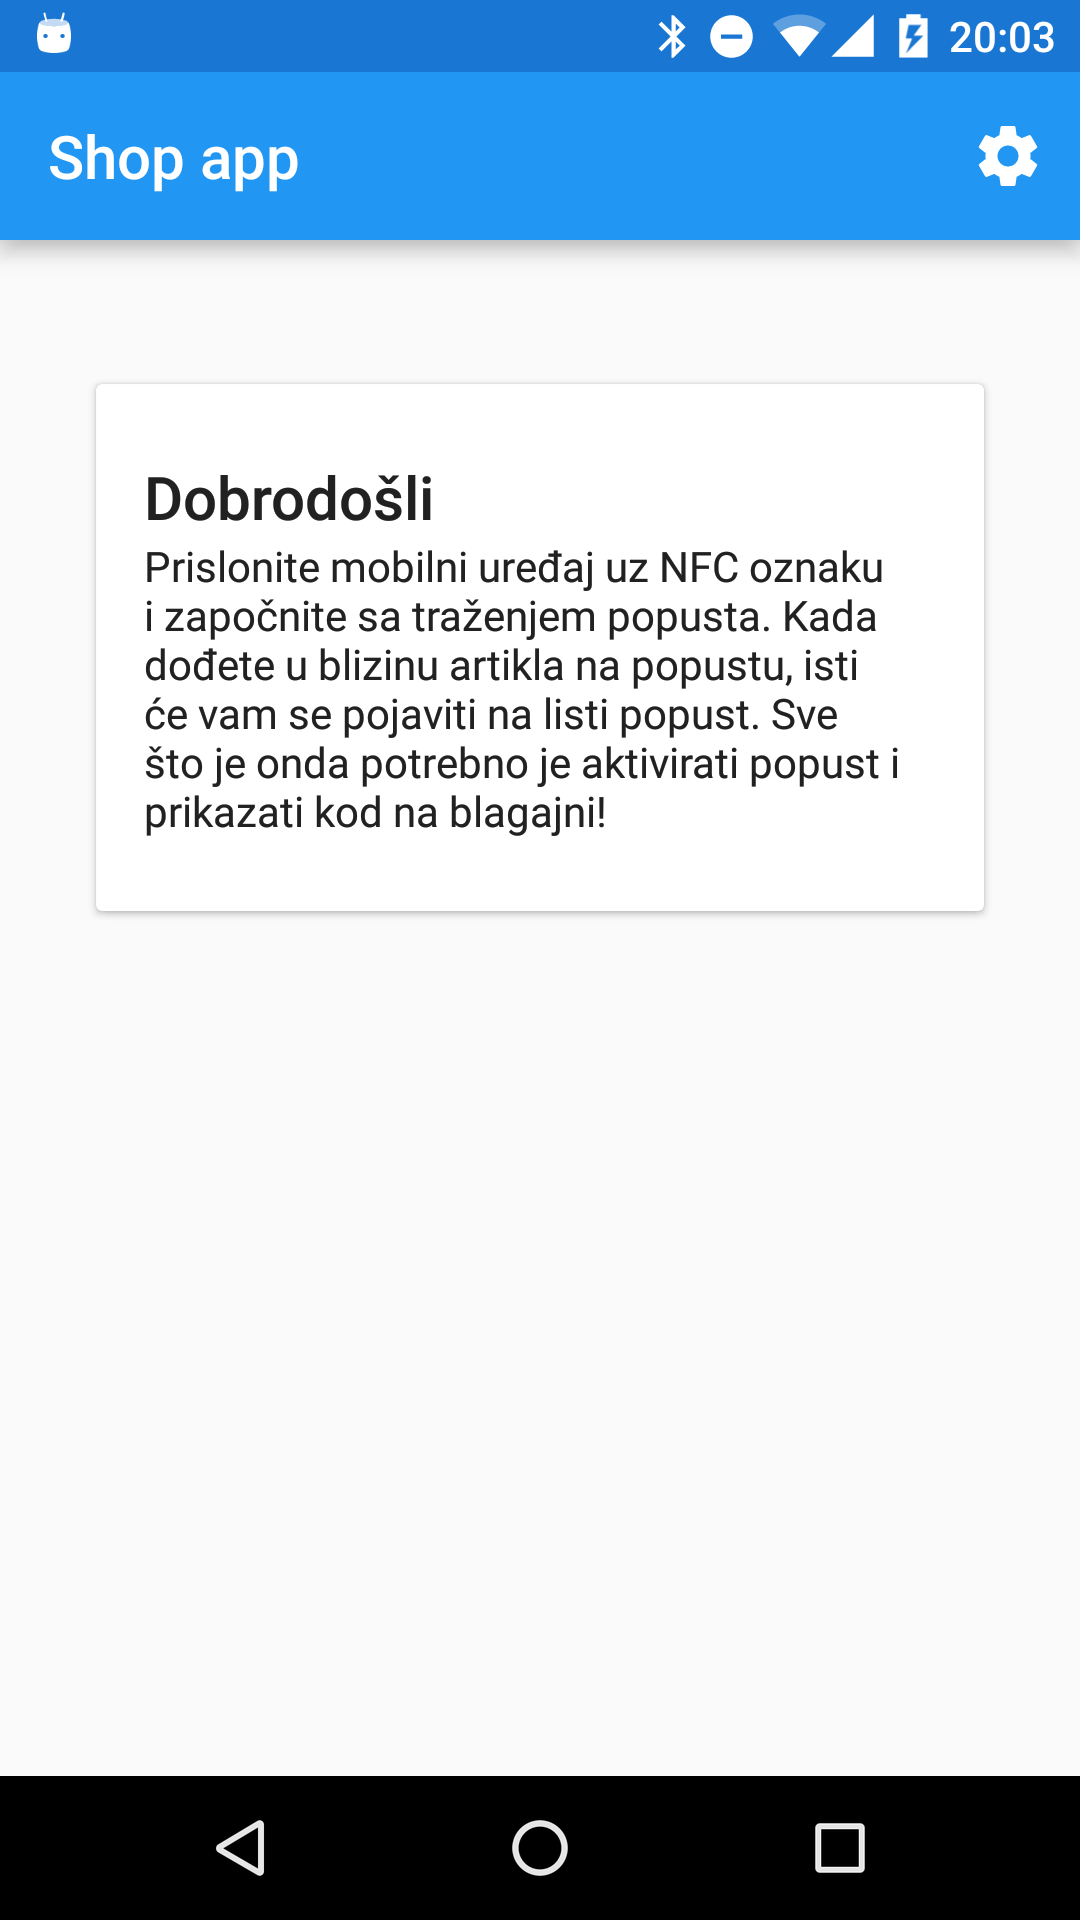
\includegraphics[height=12cm,keepaspectratio=true]{pocetni_ekran}
 \caption{Po\v{c}etni ekran}
 \label{fig:pocetniEkran}
	\end{center}
\end{figure}


\subsection{Ekran poslovnice}

Kada korisnik skenira NFC nalijepnicu otvara se ekran poslovnice i \v{c}ita se identifikacija poslovnice, pomo\'{c}u ranije opisanog mehanizma. Nakon uspje\v{s}nog \v{c}itanja identifikacije radi se zahtjev za konfiguracijom poslovnice prema poslu\v{z}itelju. Poslu\v{z}itelj vra\'{c}a osnovne informacije o poslovnici te popis popusta vezanih uz ogla\v{s}iva\v{c}e i time je zavr\v{s}en proces inicijalizacije.

Slika \ref{fig:poslovnica} prikazuje inicijalizirani ekran te dodatne informacije o poslovnici, dostupne na klik ikone informacija.



\begin{figure}[!htbp]
	\begin{center}
 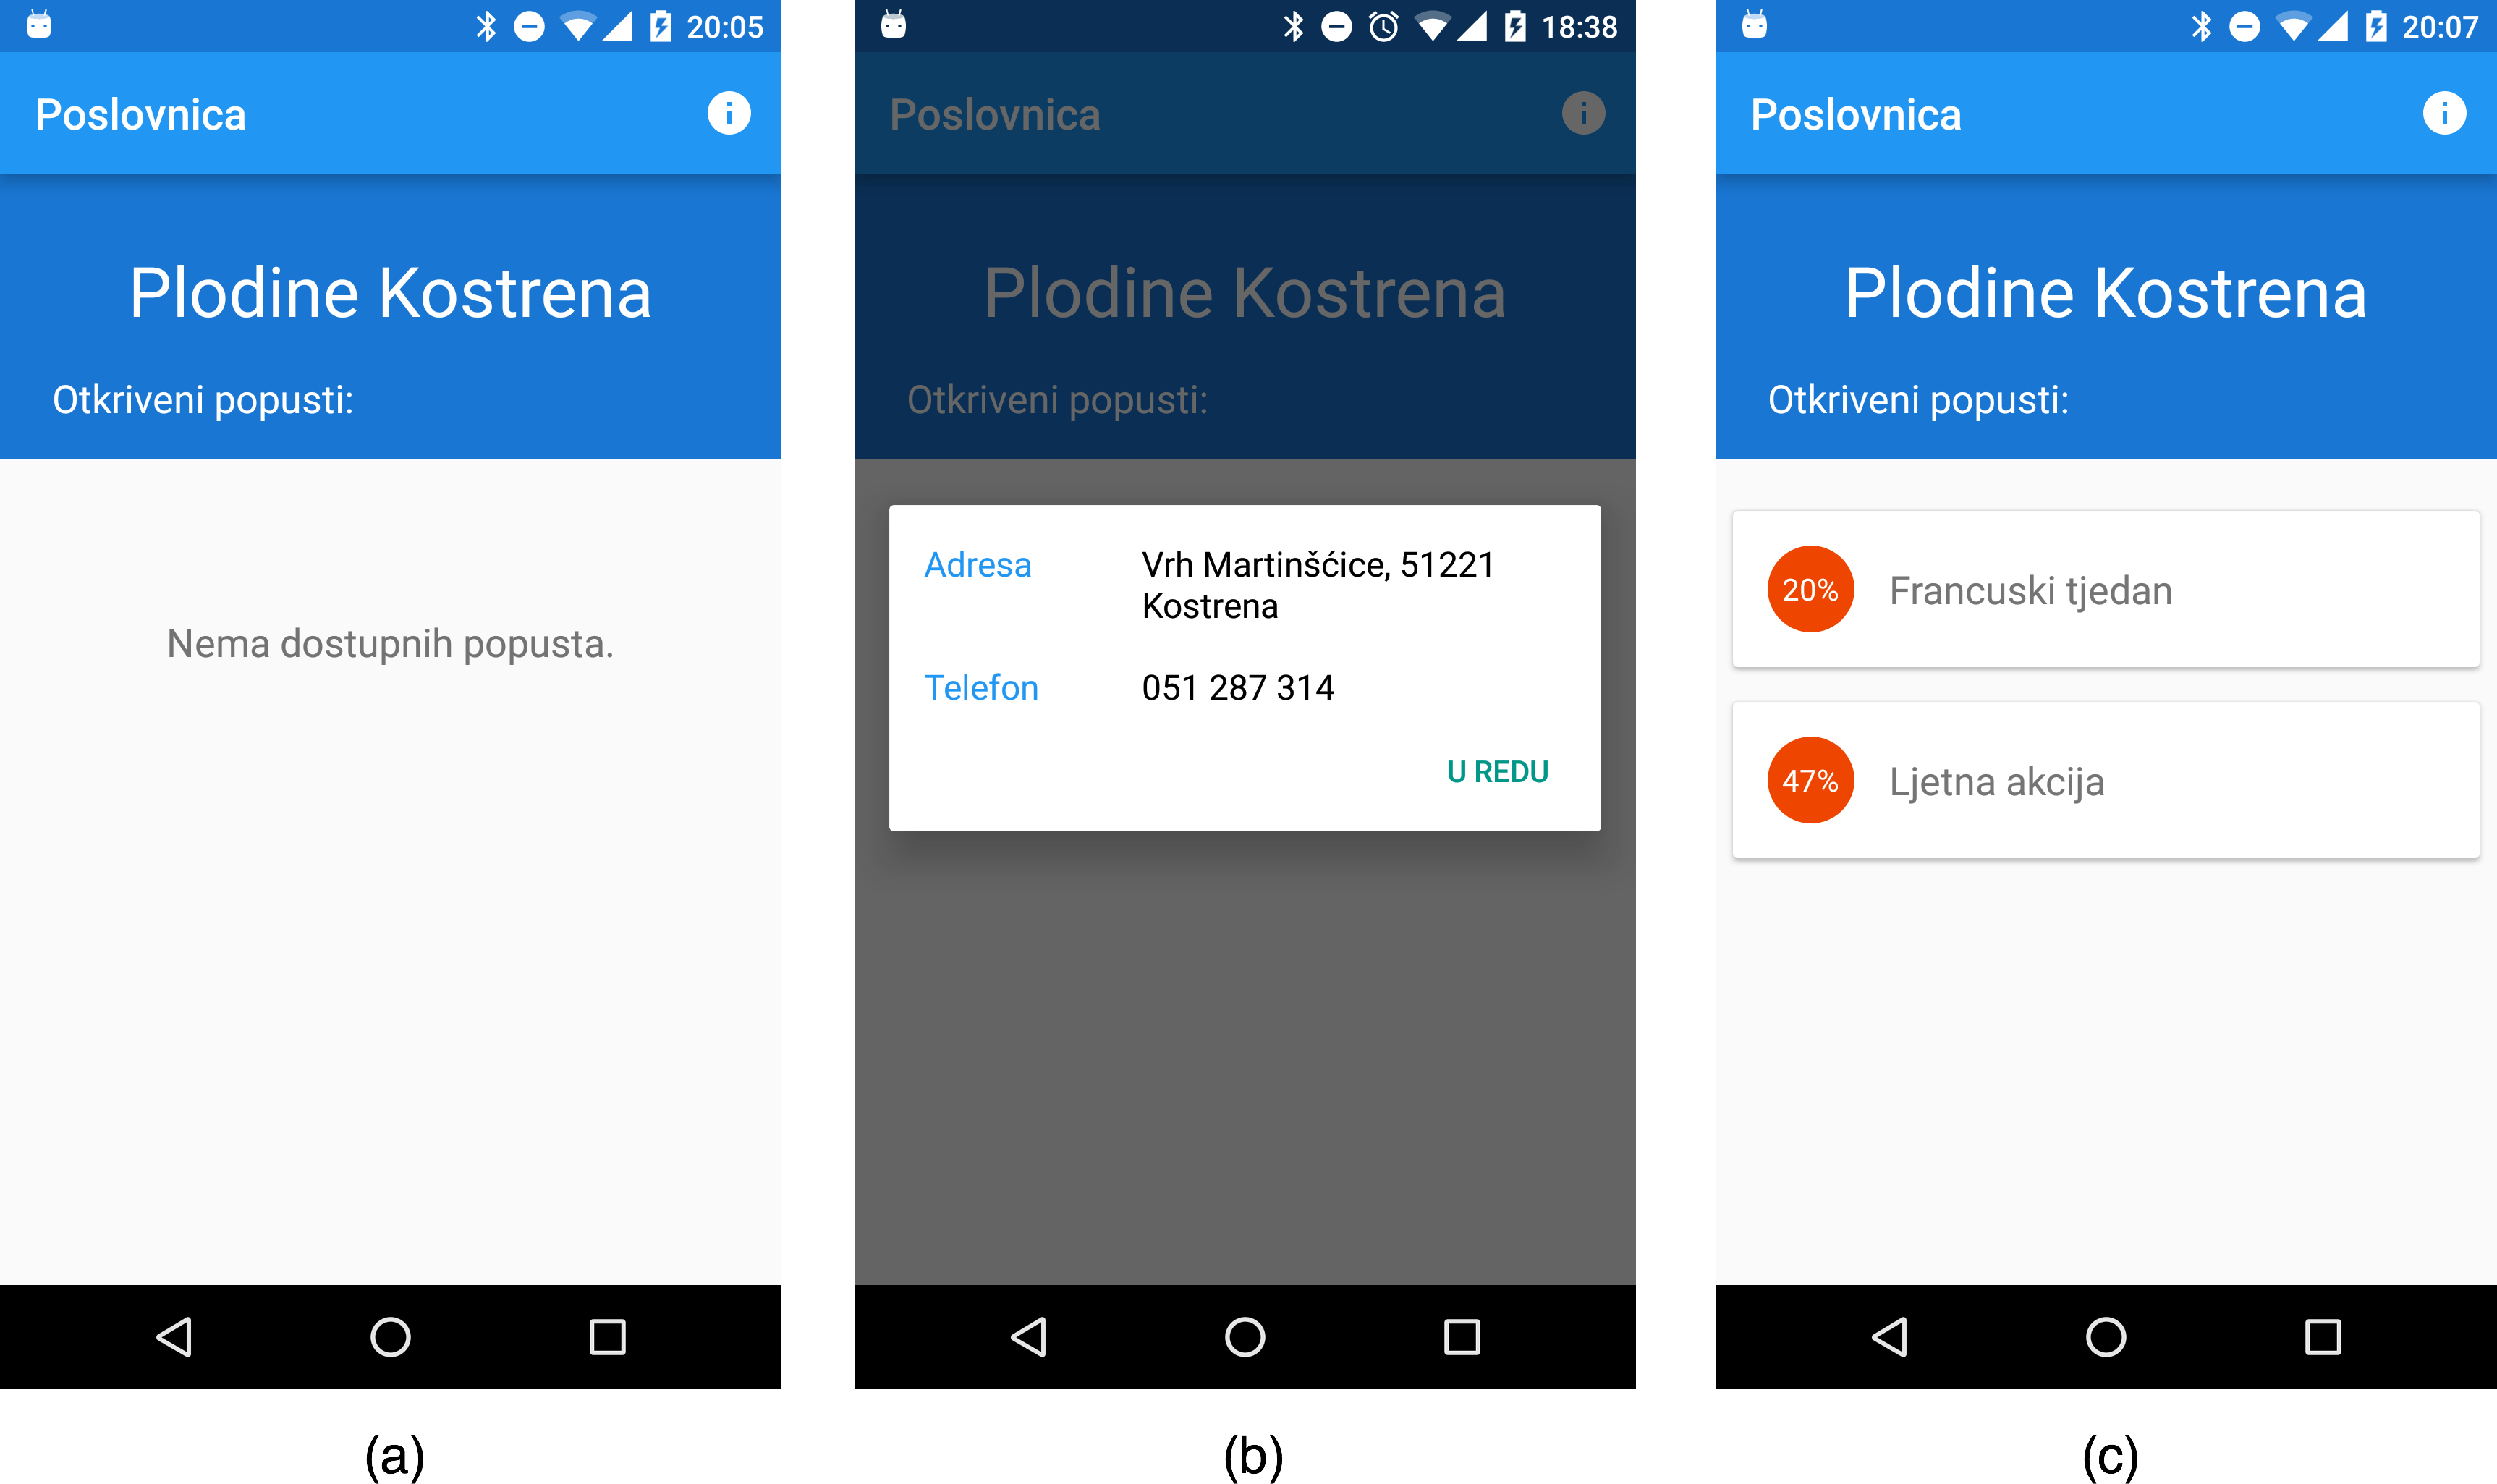
\includegraphics[height=9cm,keepaspectratio=true]{poslovnica}
 \caption{Prikaz inicijaliziranog ekrana poslovnice (a), informacija poslovnice (b) i ekrana poslovnice sa otkrivenim popustima (c)}
 \label{fig:poslovnica}
	\end{center}
\end{figure}

Kada je poslovnica inicijalizirana po\v{c}inje potraga za ogla\v{s}iva\v{c}ima pomo\'{c}u opisane BLE komunikacije. Metoda za uspje\v{s}ni pronalazak ogla\v{s}iva\v{c}a biva pozvana svaki put kada telefon detektira oglaiva\v{c} (konstantno se poziva dokle god je ogla\v{s}iva\v{c} u dometu telefona) te je zato implementirana logika pam\'{c}enja pronalazaka. Stoga, kada ogla\v{s}iva\v{c} bude prona\dj en prolazi se kroz popis popusta poslovnice te se uspore\dj uju zadana strojna adresa ogla\v{s}iva\v{c}a vezanog za popust i strojna adresa prona\dj enog ogla\v{s}iva\v{c}a. Ukoliko su jednake i popust jo\v{s} nije prikazan, popust se dodaje na listu popusta. Time je postignuta funkcionalnost da se korisniku puni lista popusta dok \v{s}eta kroz poslovnicu, koja je tak\dj er prikazana na slici \ref{fig:poslovnica}. Kada korisnik klikne na neki od popusta prikazujem mu se ekran detalja popusta.


\subsection{Ekran detalja popusta}

Kada korisnik prvi put otvori ekran detalja odgovaraju\'{c}eg popusta prikazani su mu detalji popusta u obliku jedan detalj jedna kartica. Detalji sastoje od imena proizvoda, stare i nove cijene, postotaka popusta i datuma isteka popusta. Ukoliko nije aktivirao popust, korisniku je predstavljen omogu\'{c}eni FAB gumb (univerazlna Android komponenta za aktiviranje glavne akcije ekrana, definirana u Material design specifikaciji \cite{materialDesign}) koji slu\v{z}i za kreiranje zahtjeva za kodom popusta. Prilikom kreiranja zahtjeva \v{c}ita se identifikator ure\dj aja (koriste\'{c}i Andorid-ovu klasu TelephonyManager \cite{telephonyManager} koja u ovisnosti o dostupnosti vra\'{c}a IMEI, MEID ili ESN broj koji je jednozna\v{c}an za svaki ure\dj aj) s ciljem ograni\v{c}avanja izdanih kodova na jedan po ure\dj aju. Ukoliko je zahtjev uspje\v{s}an korisnik je o tome obavje\v{s}ten odgovaraju\'{c}om porukom te mu se na detaljima popusta pojavljuje nova kartica koja sadr\v{z}i kod kojeg je du\v{z}an prikazati na blagajni. Na slici \ref{fig:detalji_poslovnice} je prikazan opisan ekran i stanja u kojima se mo\v{z}e nalaziti.



\begin{figure}[!htbp]
	\begin{center}
 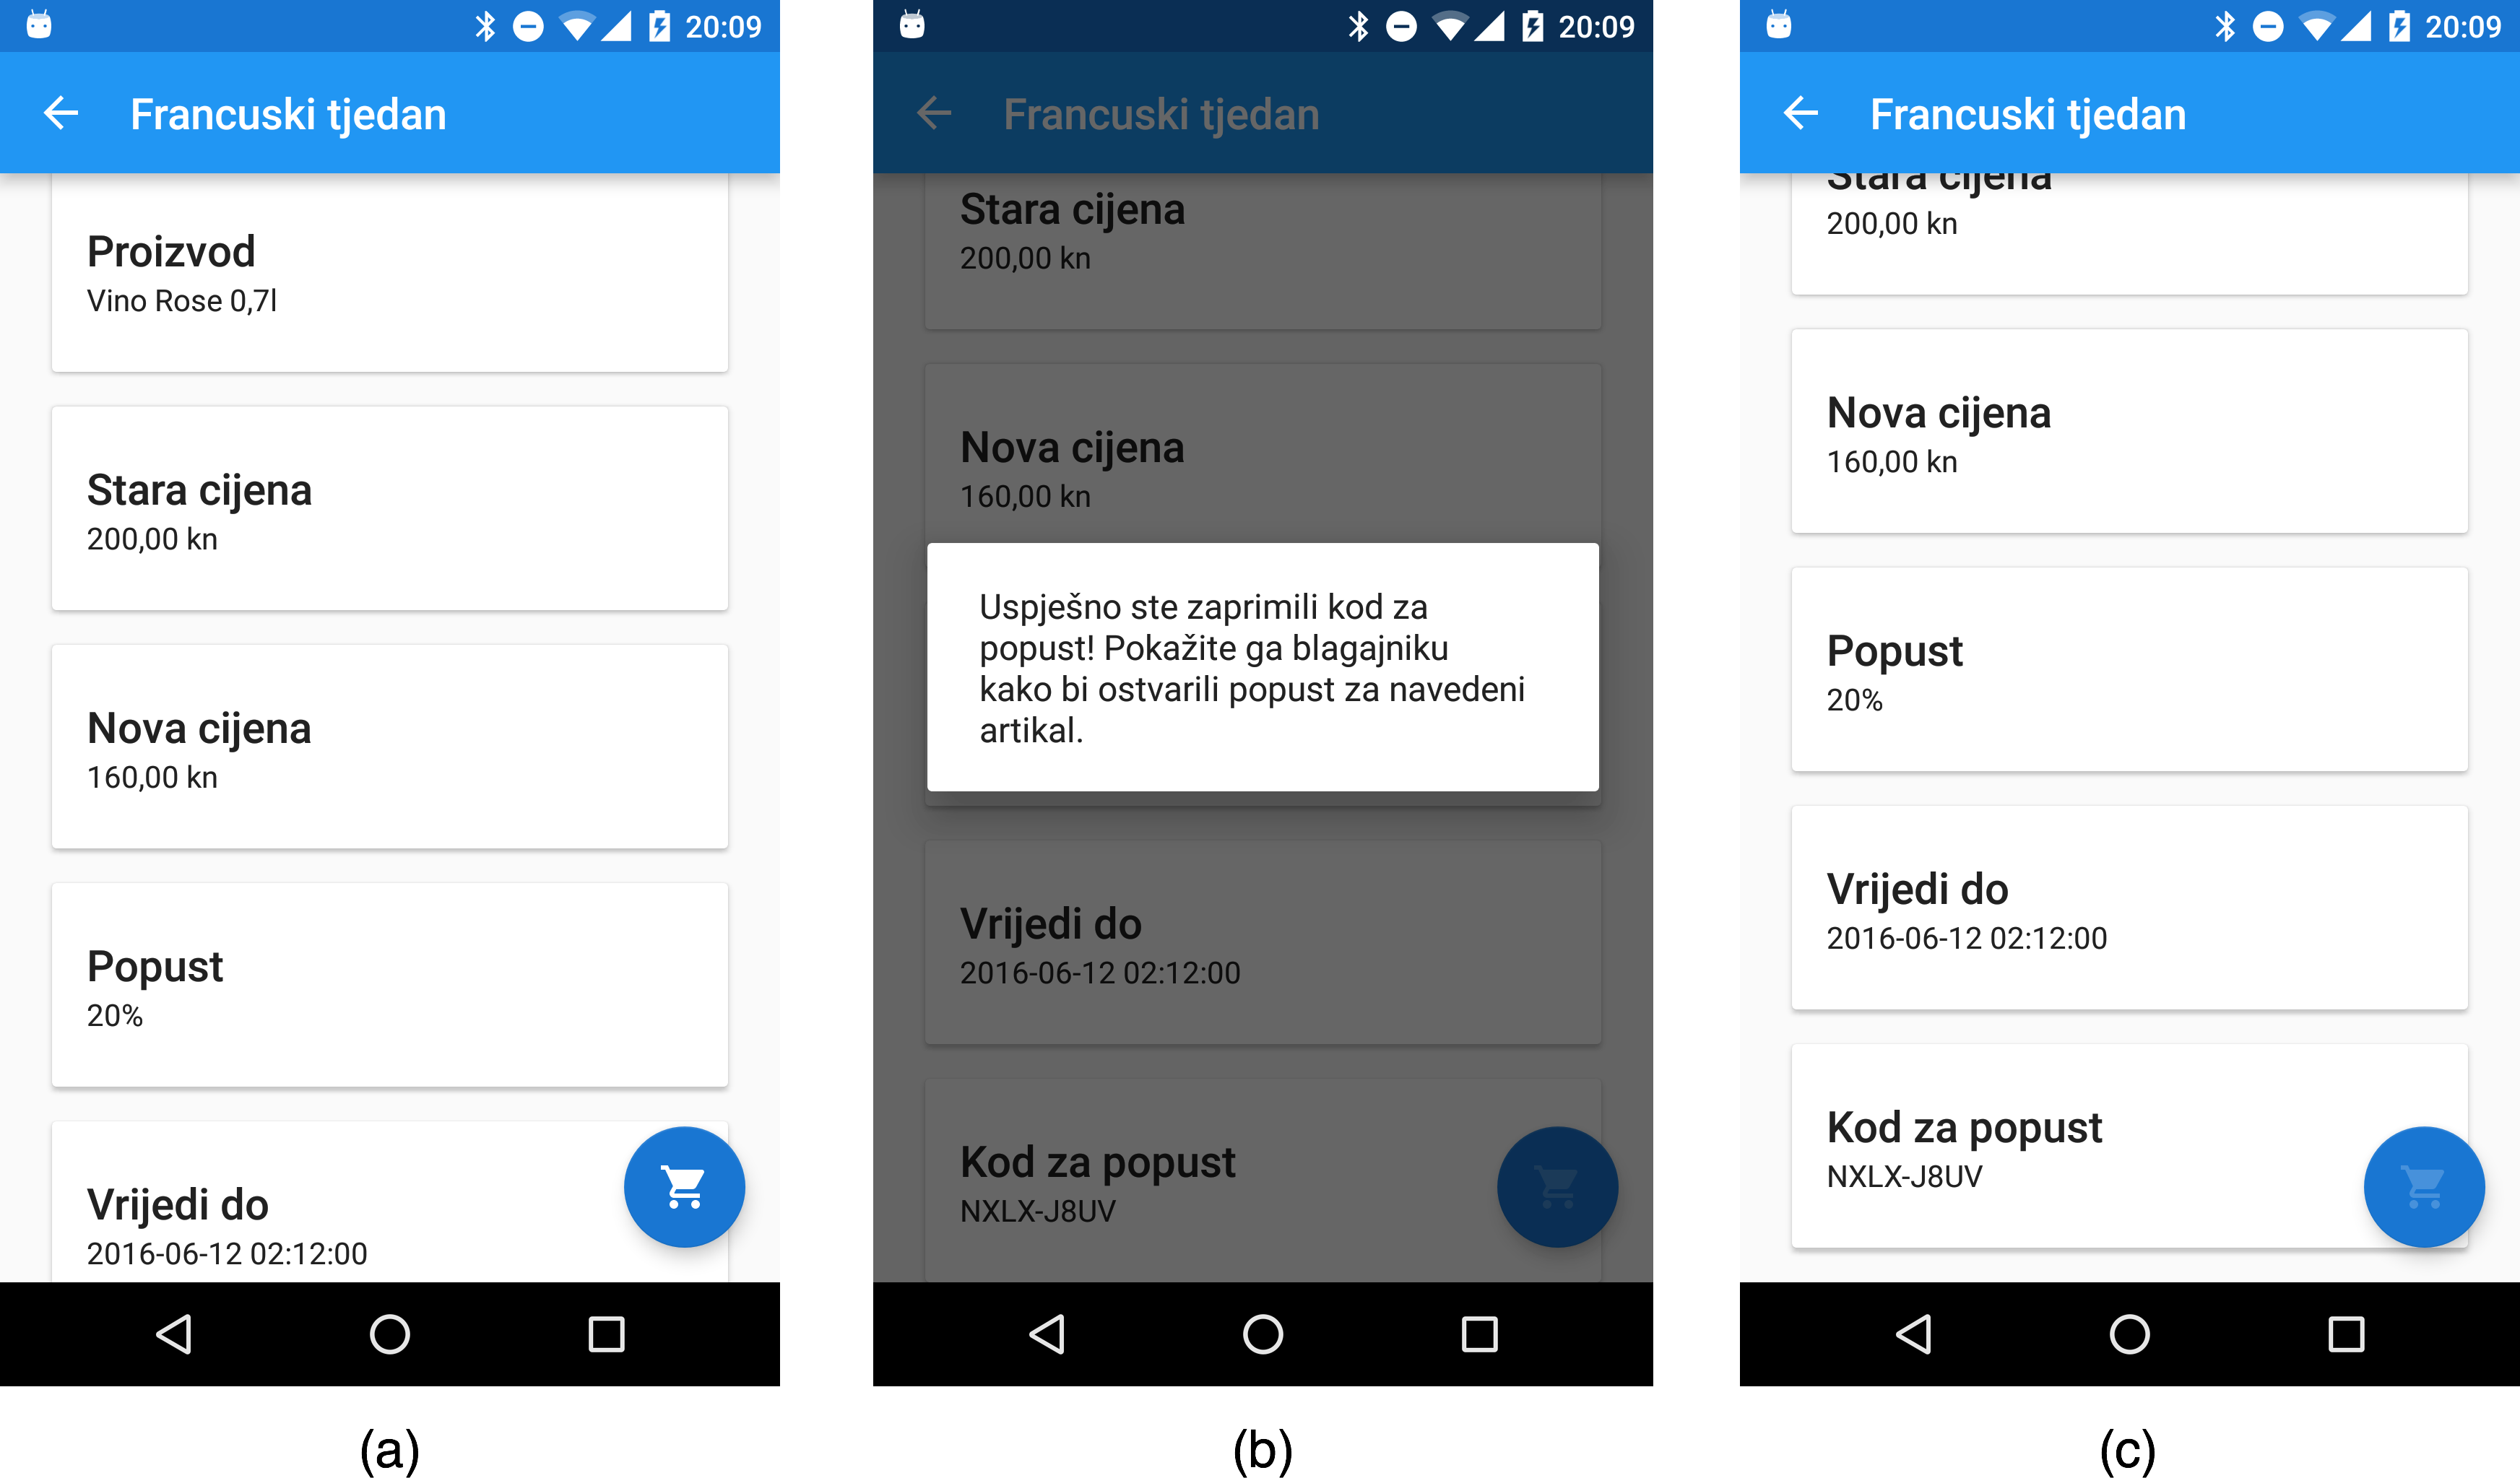
\includegraphics[height=9cm,keepaspectratio=true]{detalji_poslovnice}
 \caption{Slika sadr\v{z}i prikaz inicijalnog ekrana sa detaljima popusta (a), poruka uspje\v{s}nog primanja koda (b) i ekran sa detaljima popusta koji uklju\v{c}uje i kod za popust (c)}
 \label{fig:detalji_poslovnice}
	\end{center}
\end{figure}


\subsection{Ekran postavki}
Ekran popusta sadr\v{z}i opciju za postavljanje gornje granice ja\v{c}ine signala BLE ogla\v{s}iva\v{c}a koja je dovoljna da aplikacija detektira ogla\v{s}iva\v{c}. Granica ozna\v{c}ava numeri\v{c}ku vrijednost u decibelima te se prilikom detekcije BLE ogla\v{s}iva\v{c}a evaluira vrijednost detekiranog signala te ukoliko je unutar unutrar zadane granice, aplikacija nastavlja sa obra\dj ivanjem BLE ogla\v{s}iva\v{c}a.
Odabrana numeri\v{c}ka vrijednost se zapisuje u internu memoriju pametnog telefona te ona biva dostupna i nakon \v{s}to aplikacija prestane sa radom. Slika \ref{fig:postavke} prikazuje ekran postavki.


\begin{figure}[!htbp]
	\begin{center}
 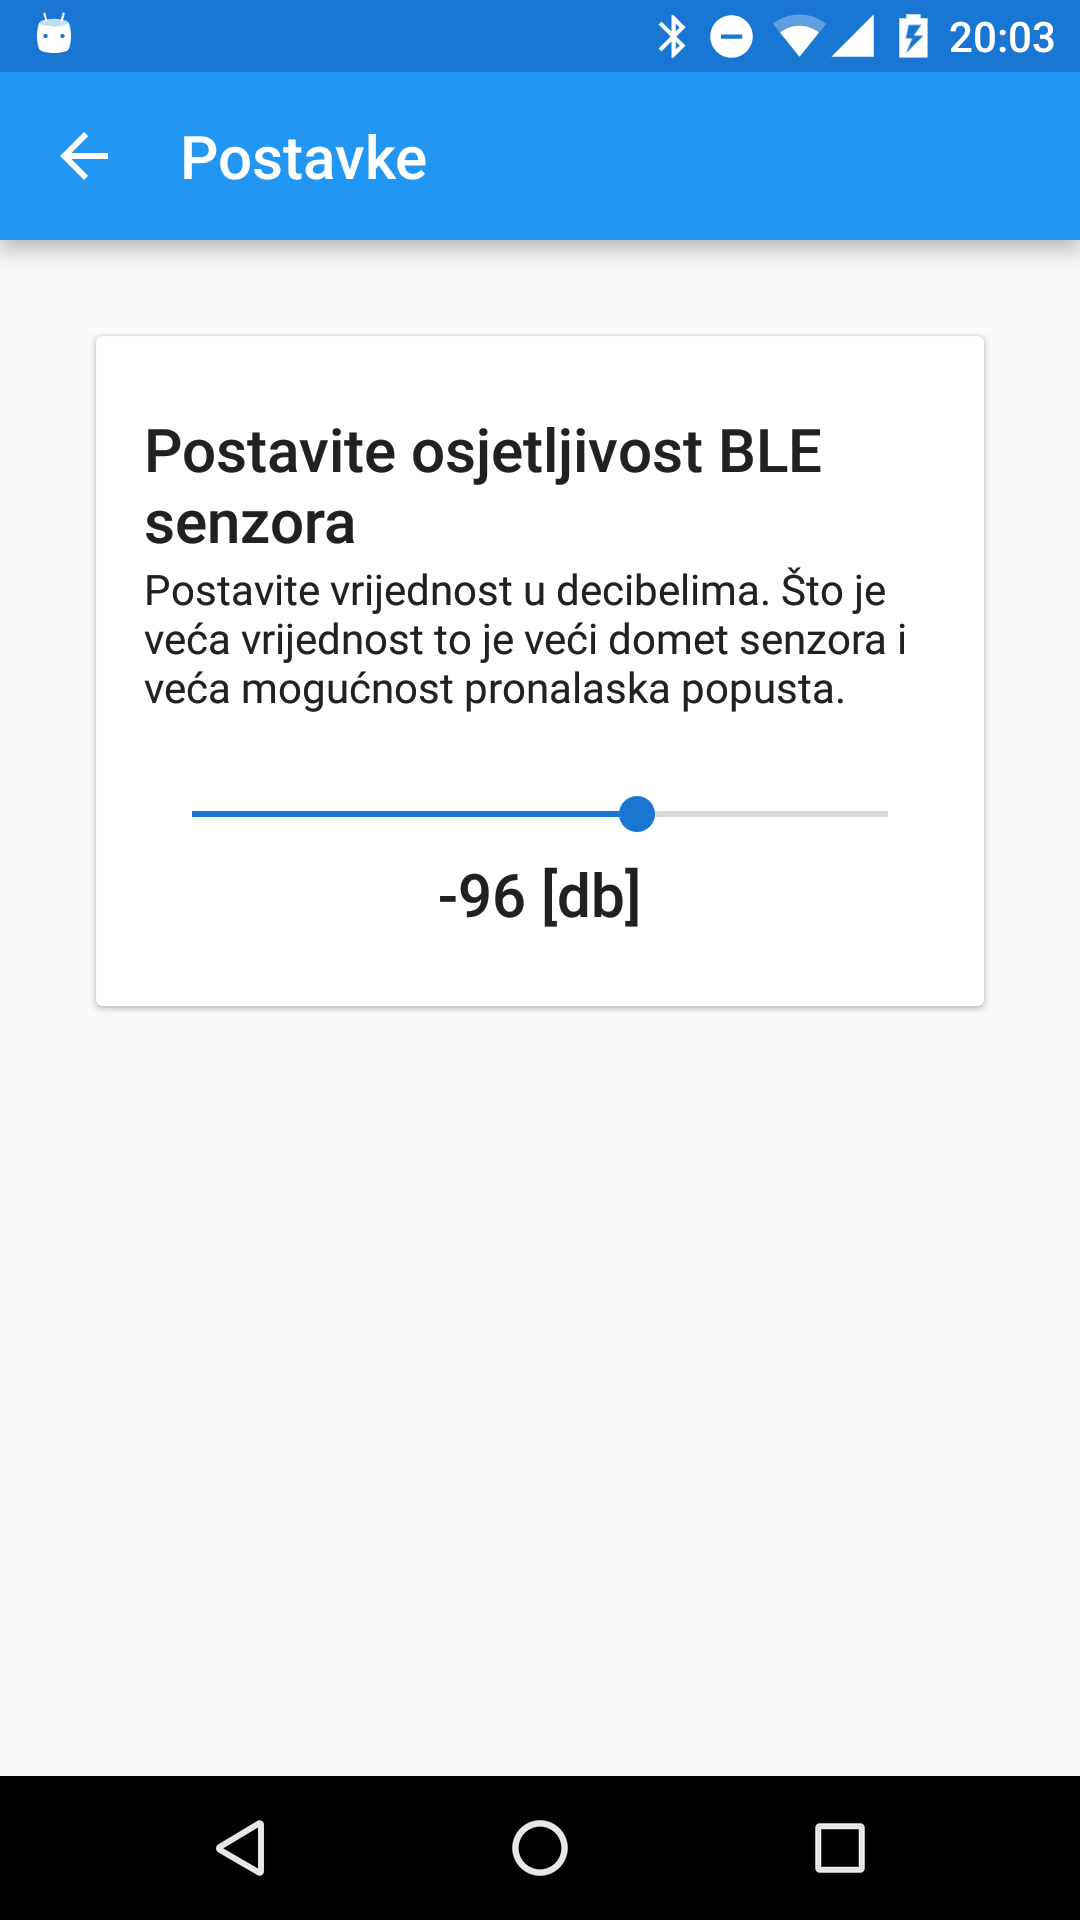
\includegraphics[height=12cm,keepaspectratio=true]{postavke}
 \caption{Ekran postavki u kojemu je korisniku dopu\v{s}teno odabrati gornju granicu ja\v{c}ine signala, dovoljnog za detekciju od strane aplikacije}
 \label{fig:postavke}
	\end{center}
\end{figure}


\section{Kori\v{s}tene knji\v{z}nice}

Knji\v{z}ica ozna\v{c}ava skup resusra koji se dodaju u izvorni kod projekta, a slu\v{z}e za pru\v{z}anje odre\dj enih funkcionalnosti. Uklju\v{c}ivanjem knji\v{z}nica u projekt se mo\v{z}e bitno skratiti vrijeme potrebno za razvoj jer nije potrebno implemntirati ne\v{s}to \v{s}to je netko ve\'{c} implementirao, dobro testirao i pru\v{z}io tr\v{z}i\v{s}tu. S druge strane, dodavanjem knji\v{z}nice se dobivamo sve funkcionalnosti iste koje mo\v{z}da nisu potrebne a mogu pove\'{c}ati veli\v{c}inu projekta (potencijalni problem kod Androida jer ljudi generalno ne vole aplikacije koje zauzimaju puno memorije).
Dodavanje knji\v{z}ica se u Android-u se radi preko Gradle priklju\v{c}ka \cite{gradle} koji slu\v{z}i za izgradnju projekta. Proces dodavanja knji\v{z}ice uklju\v{c}uje upis lokacije knji\v{z}nice u datoteku build.gradle (konfiguracijska datoteka zapisana u programskom jeziku Groovy \cite{groovy}, koja definira izgradnju projekta). Lokacija knji\v{z}ice je zapravo ime paketa i verzija \v{z}eljene knji\v{z}ice, \v{s}to je dovoljno informacija Gradle priklju\v{c}ku da ju prona\dj e na repozitoriju jCenter \cite{jcenter} (centralni repozitor za Android knji\v{z}ice otvorenog koda) i preuzme. Tada od knji\v{z}ice postaje dostupan za kori\v{s}tenje u cijelom projektu.
Kori\v{s}tene knji\v{z}ice su:

\begin{itemize}
	\item Support design
	\begin{itemize}
		\item Google-ova slu\v{z}bena knji\v{z}ica u kojoj se nalaze komponente korisni\v{c}kog su\v{c}elja te se pru\v{z}a kompatibilnost za stare verzije Android-a
	\end{itemize}

	\item Okhttp \cite{okhttp}
	\begin{itemize}
		\item HTTP klijent za Android i Java aplikacije
		\item Koristi se za komunikaciju aplikacije sa poslu\v{z}iteljom
	\end{itemize}

	\item GSON \cite{gson}
	\begin{itemize}
		\item Knji\v{z}ica za serijalizaciju JSON objekata u Java objekte i obrnuto
		\item Koristi se serijalizaciju odgovora poslu\v{z}itelja u model
	\end{itemize}
	
	\item Butterknife \cite{butterKnife}
	\begin{itemize}
		\item Knji\v{z}ica koja uvodi anotacije koje povezuju komponentu korisni\v{c}kog su\v{c}elja definiranog u XML-u sa Java objektom, preko identifikatora
		\item Koristi se za smanjivanja linija koda i \v{c}i\v{s}\'{c}i kod
	\end{itemize}


	\item EventBus \cite{eventBus}
	\begin{itemize}
		\item Knji\v{z}ica za ogla\v{s}avanje i pretplatu na doga\dj aje
		\item Slu\v{z}i za olak\v{s}avanje komunikacije izme\dj u klasa
		\item Koristi se za obavjest o promjeni stanja BLE i internet modula na razini cijele aplikacije
	\end{itemize}
\end{itemize}





\chapter{Internetska aplikacija}

Internetska aplikacija se sastoji od korisni\v{c}kog su\v{c}elja za internetske korisnike i (API) za mobilne korisnike. Zajedni\v{c}ko objema aplikacijama je kori\v{s}tenje iste baze podataka koja slu\v{z}i kao centralni repozitorij podataka. U nastavku ovog poglavlja je prvo obja\v{s}njena struktura baze, a zatim implementacija internetske aplikacije i API su\v{c}elja.

\section{Baza podataka}

Baza podataka sastoji se od \v{s}est tablica te je modelirana po tre\'{c}oj normalnoj formi. To zna\v{c}i da su tablice kreirane i pomo\'{c}u relacijskih veza strukturirane s ciljem minimiziranja redundancije podataka. Relacijske veze uklju\v{c}uju definiranje primarnog klju\v{c}a svake tablice (atribut tablice koji ima jedinstvenu vrijednost za svaki zapis) te kreiranje stranih klju\v{c}eva (veza izme\dj u primarnog klju\v{c}a jedne tablice i atributa druge tablice). Struktura baze i veze izme\dj u tablica su prikazani na slici ~\ref{fig:bazaPodataka}.


\begin{figure}[!htbp]
	\begin{center}
 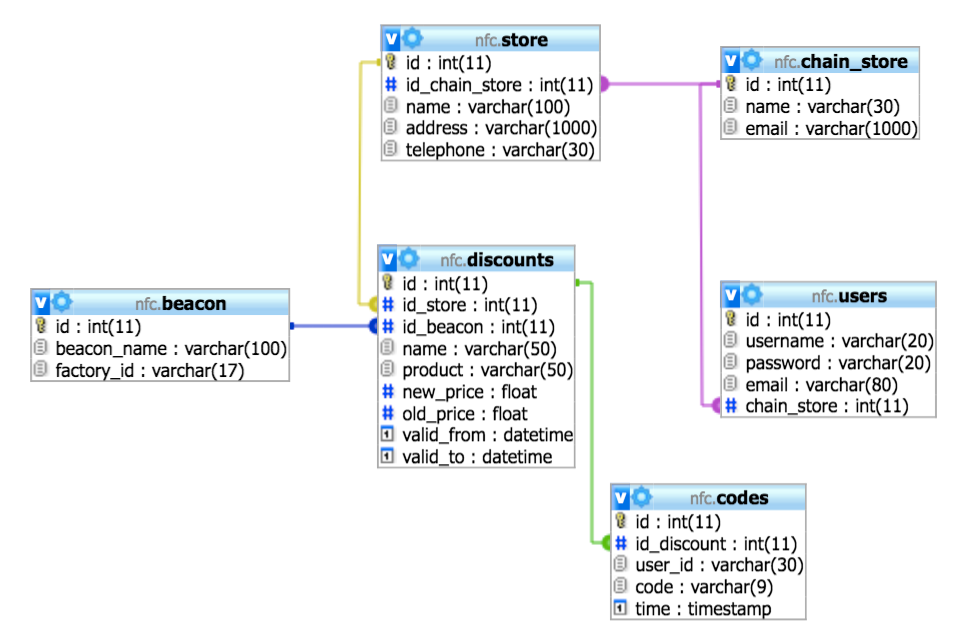
\includegraphics[height=10cm,keepaspectratio=true]{web_baza}
 \caption{Struktura baze podataka}
 \label{fig:bazaPodataka}
	\end{center}
\end{figure}

Baza podataka se sastoji od sljede\'{c}ih tablica:
\begin{itemize}
	\item Lanac trgovina
	\begin{itemize}
		\item Sadr\v{z}i naziv i e-mail adresu lanca trgovina
	\end{itemize}
	\item Poslovnica
	\begin{itemize}
		\item Sadr\v{z}i osnovne informacije o poslovnici i referencu na lanac trgovina
	\end{itemize}
	\item Popust
	\begin{itemize}
		\item Sadr\v{z}i osnovne informacije o popustu i referencu na poslovnicu i ogla\v{s}iva\v{c}
	\end{itemize}
	\item Ogla\v{s}iva\v{c}
	\begin{itemize}
		\item Sadr\v{z}i naziv i strojnu adresu ogla\v{s}iva\v{c}a
	\end{itemize}
	\item Kod za popust
	\begin{itemize}
		\item Sadr\v{z}i kod, vrijeme aktivacije i identifikator korisnika te referencu na popust
	\end{itemize}
	\item Korisnik
	\begin{itemize}
		\item Korisnik internetske aplikacije, vezan je za lanac trgovina
	\end{itemize}
\end{itemize}



\section{Internetska aplikacija}

\subsection{Su\v{c}elje za pristup}

Prvo \v{s}to korisnik vidi kada preko pretra\v{z}iva\v{c}a ode na lokaciju internetske aplikacije je forma za unos kredencija, prikazana na slici ~\ref{fig:webLogin}. Korisnik je du\v{z}an unijeti svoje korisni\v{c}ko ime i lozinku, kako bi pristupio po\v{c}etnom su\v{c}elju.

\begin{figure}[!htbp]
	\begin{center}
 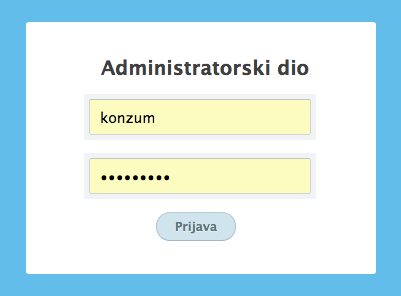
\includegraphics[height=5cm,keepaspectratio=true]{web_login}
 \caption{Forma za unos kredencija}
 \label{fig:webLogin}
	\end{center}
\end{figure}


\subsection{Po\v{c}etno su\v{c}elje}

Nakon uspje\v{s}nog pristupanja aplikaciji, korisniku je prikazano po\v{c}etno su\v{c}elje na slici ~\ref{fig:web_glavni}. Su\v{c}elje se sastoji od izbornika, centralnog dijela i tipke za odjavu iz sustava. U izborniku se nalaze glavne korisni\v{c}ke opcije koje uklju\v{c}uju popis poslovnica, su\v{c}elje za kreiranje popusta i su\v{c}elje za kreiranje nove poslovnice.


\begin{figure}[!htbp]
	\begin{center}
 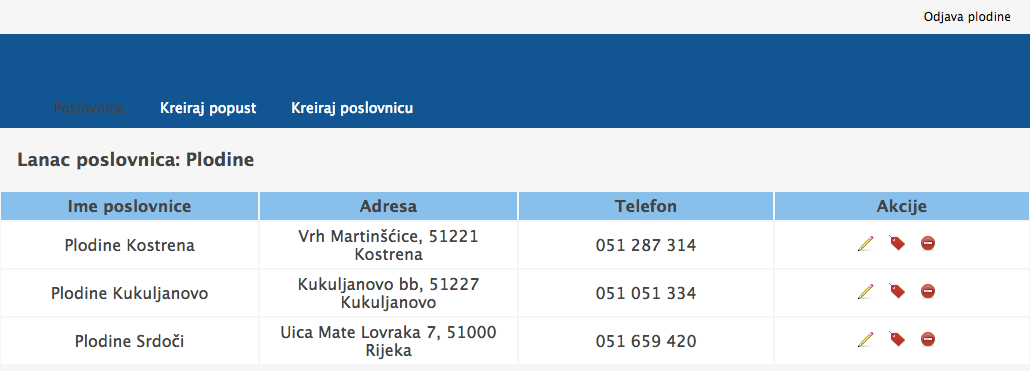
\includegraphics[height=5cm,keepaspectratio=true]{web_glavni}
 \caption{Popis poslovnica trgova\v{c}kog lanca}
 \label{fig:web_glavni}
	\end{center}
\end{figure}

Kada se korisnik prijavi u sustav u centralnom dijelu su\v{c}elja mu se prika\v{z}e popis poslovnica trgova\v{c}kog lanca za koji je vezan. Popis je prikazan u formatu tablice te osim osnovnih informacija o poslovnicama uklju\v{c}uje i akcije vezane za poslovnicu. Dostupne akcije su ure\dj enje poslovnice, pregledavanje popusta poslovnice i brisanje poslovnice.


\subsection{Poslovnica}

U aplikaciji je implementirano dodavanje, ure\dj ivanje i brisanje poslovnice, a odgovaraju\'{c}a su\v{c}elja su prikazana na slici ~\ref{fig:web_poslovnicaa}.

\begin{figure}[!htbp]
	\begin{center}
 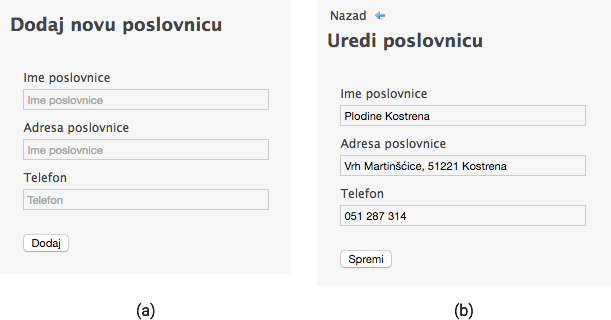
\includegraphics[height=7cm,keepaspectratio=true]{web_poslovnicaa}
 \caption{Dodavanje i ure\dj ivanje poslovnice}
 \label{fig:web_poslovnicaa}
	\end{center}
\end{figure}

Korisnik sa popisa poslovnica mo\v{z}e odabrati i pregled popusta poslovnice, te mu se tada u centralnom dijelu su\v{c}elja prikazuju svi popusti poslovnice prikazani na slici ~\ref{fig:web_popusti}.

\begin{figure}[!htbp]
	\begin{center}
 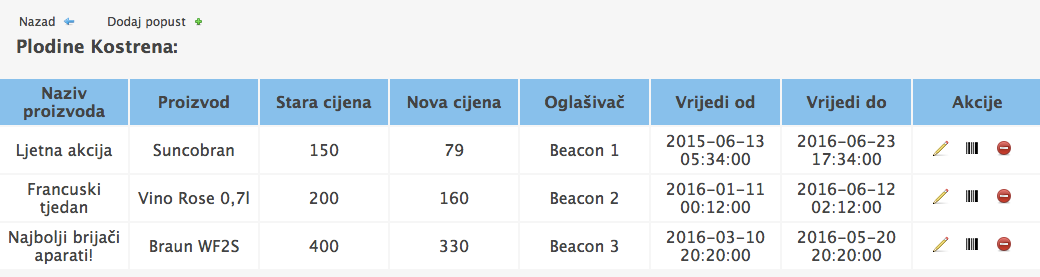
\includegraphics[height=3.9cm,keepaspectratio=true]{web_popusti}
 \caption{Popusti poslovnice}
 \label{fig:web_popusti}
	\end{center}
\end{figure}

Popusti su strukturirani u tablicu iz koje korisnik mo\v{z}e pro\v{c}itati podatke o popustu, kao i napraviti akcije koje uklju\v{c}uju ure\dj ivanje i brisanje popusta te pregled aktivacijskih kodova poslovnice.


\subsection{Popust}

Korisniku je omogu\'{c}eno kreiranje, ure\dj ivanje i brisanje popusta. Na slici ~\ref{fig:web_dodaj_popust} su prikazane forme za kreiranje i ure\dj ivanje popusta.

\begin{figure}[!htbp]
	\begin{center}
 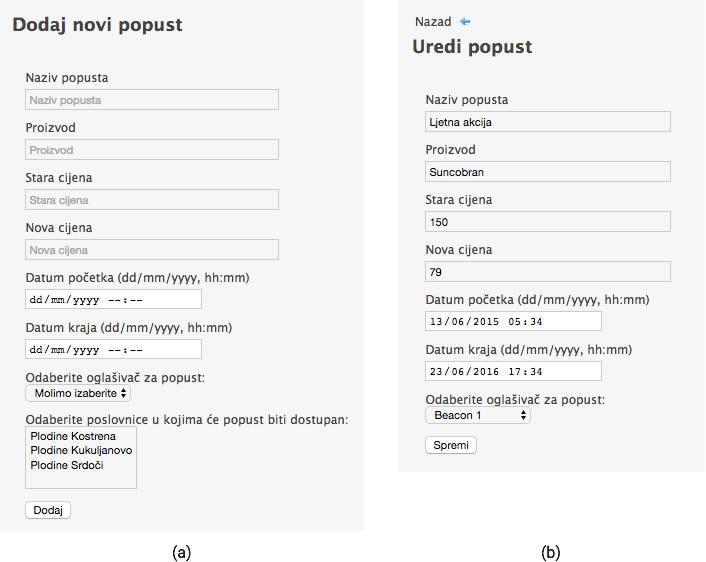
\includegraphics[height=10cm,keepaspectratio=true]{web_dodaj_popust}
 \caption{Popusti poslovnice}
 \label{fig:web_dodaj_popust}
	\end{center}
\end{figure}
Kod kreiranja popusta je potrebno unijeti osnovne informacije o popustu koje uklju\v{c}uju i ogla\v{s}iva\v{c} za kojeg je popust vezan, kao i poslovnice u kojim se popust mo\v{z}e ostvariti. Kod ure\dj ivanja popusta koji je ve\'{c} vezan za poslovnicu korisnik mo\v{z}e, uz osnovne informacije, promijeniti samo ogla\v{s}iva\v{c} za kojeg je popust vezan.


\subsection{Pregled kodova popusta}
Za svaki popust u poslovnici je omogu\'{c}eno i pregledavanje kodova koji su izdani za popuste. Primjer aktiviranih kodova je prikazan na slici ~\ref{fig:web_kodovi}.

\begin{figure}[!htbp]
	\begin{center}
 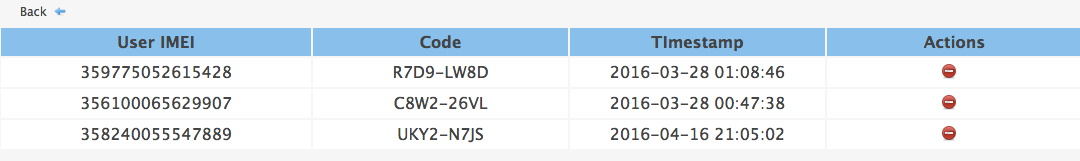
\includegraphics[height=2.2cm,keepaspectratio=true]{web_kodovi}
 \caption{Aktivirani kodovi popusta}
 \label{fig:web_kodovi}
	\end{center}
\end{figure}

Na su\v{c}elju su prikazane informacije o popustu koje uklju\v{c}uju identifikator korisnika (IMEI broj njegovog pametnog telefona), aktivacijski kod, vrijeme aktiviranja koda i opcija brisanja aktivacije.

\subsection{API su\v{c}elje}

API su\v{c}elje ozna\v{c}ava skup pravila komunikacije kojeg koriste dva ra\v{c}unalna sustava kako bi razmijenili informacije. U sklopu ovog projekta je su\v{c}elje moralo biti implementirano kako bi mobilna aplikacija mogla komunicirati sa bazom podataka koju koristi internetska aplikacija. Komunikacija se vr\v{s}i tako da mobilna aplikacija radi API zahtjev sa ispravnom metodom (GET ili POST) na ispravnu internetsku lokaciju. Ovisno o tipu komunikacije, zahtjev mora sadr\v{z}avati odre\dj ene podatke kako bi su\v{c}elje moglo napraviti ispravan zahtjev prema bazi (primjer je aktivacija popusta pri \v{c}emu je mobilna aplikacija u zahtjevu du\v{z}na poslati ure\dj ajev IMEI). Kada su podaci izvu\v{c}eni iz baze podataka, potrebno ih je serijalizirati u format koji je podoban za slanje i kojeg primatelj zna interpretirati. Za potrebe ove aplikacije je kori\v{s}ten JSON format \cite{json} (JavaScript Object Notation), koji specificira podatke kao kolekciju parova ime-vrijednost. Vrijednost mo\v{z}e biti primitiv, objekt i lista primitiva/objekta. Na slici ~\ref{fig:web_json} je prikazana konfiguracija poslovnice koja se \v{s}alje preko API-a, u JSON formatu.


\begin{figure}[!htbp]
	\begin{center}
 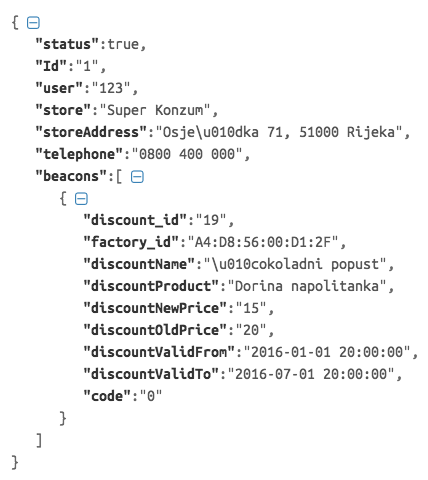
\includegraphics[height=9cm,keepaspectratio=true]{web_json}
 \caption{Aktivirani kodovi popusta}
 \label{fig:web_json}
	\end{center}
\end{figure}

 
\chapter{Usporedba NFC-a i BLE-a}


BLE i NFC su dva be\v{z}i\v{c}na komunikacijska protokola te ovo poglavlje slu\v{z}i kao usporedba istih. Po\v{s}to su zanovani na razli\v{c}itim tehnologijama, protokoli imaju razli\v{c}ite karakteristike i razli\v{c}itu primjenu. 
Nastavak poglavlja je koncipiran kao usporedba opisanih protokola u kontekstu dometa, sigurnosti, potro\v{s}nje energije, cijene i primjene. 

\subsubsection{Domet}

BLE tehnologija mjeri svoj domet u metrima (u praksi do 10 metara) a NFC tehnologija mjeri svoj domet u centimetrima (do 10 centimetara). Iz dometa protokola je vidljivo da BLE pru\v{z}a korisnicima ve\'{c}u fleksibilnost pri kori\v{s}tenju, dok je kod NFC-a korisnik primoran prisloniti svoj ure\dj aj na NFC ure\dj aj. Projektant sustava koji se bazira na ovim tehnologijama moraja biti svjestan ograni\v{c}enja koje pru\v{z}aju protokoli i shodno tome mora postaviti ure\dj aje u prostoru na na\v{c}in da kori\v{s}tenje korisnicima bude \v{s}to jednostavnije.

\subsubsection{Sigurnost}

BLE koristi uparivanje ure\dj aja i enkripciju (128 bitnu AES kriptografiju) prilikom oda\v{s}iljanja podataka  \cite{bleSecurity}, iako kod kori\v{s}tenja protokola u obiliku ogla\v{s}iva\v{c}a i nema velikih sigurnosnih rizika jer je svrha ure\dj aja samo ogla\v{s}avati svoje prisutstvo u prostoru.  Po\v{s}to se NFC koristi za delikatnije transakcije (recimo pla\'{c}anje sa kreditnom karticom) sigurnost je tu ve\'{c}i problem nego kod BLE-a . Postoje rizici od prislu\v{s}kivanja transakcije, manipulacije podataka koji se prenose kroz komunikacijski kanal i kra\dj e ure\dj aja i vr\v{s}enja ne\v{z}eljenih transakcija \cite{nfcSecurity}. Navedeni problemi se rje\v{s}avaju osiguravanjem sigurnog kanala izme\dj u NFC ure\dj aja (pomo\'{c}u Diffie-Hellmann algoritma) i enkripcije podataka koji se razmjenjuju (3DES ili AES kriptografija ili ) \cite{nfcSecurityTwo}. Tako\dj er, korisnik protokola ima va\v{z}nu ulogu u sigurnosti jer je domet kratak pa mo\v{z}e uo\v{c}iti nepravilnosti u komunikaciji.

\subsubsection{Potro\v{s}nja energije}
Oba protokola tro\v{s}e jednako struje u kori\v{s}tenju (oko 15 mA), dok NFC tro\v{s}i ne\v{s}to manje energije u stanju mirovanja (BLE oko \SI{1}{\micro\ampere} a NFC manje of \SI{1}{\micro\ampere}) \cite{mobilePayments}. Navedeni iznosi potro\v{s}nje energije kod oba protokola zaista malena u usporedbi sa drugim be\v{z}i\v{c}nim komunikacijskim protokolima.


\subsubsection{Cijena}
Generalno cijene modula za oba protokola su relativno niske i time su pristupa\v{c}ni proizvo\dj a\v{c}ima da ih integrirju u svoje proizvode, s time da su NFC ure\dj aji jeftiniji. NFC naljepnice kori\v{s}tene u ovom projektu su ko\v{s}tale 7.67 kn po naljepnici \cite{whiztags}, dok su BLE ogla\v{s}iva\v{c}i ko\v{s}tali 33.06 kn po komadu \cite{gimbal_beacon}.

\subsubsection{Dostupnost}
Oba protokola su danas prili\v{c}no dostupna prosje\v{c}nom \v{c}ovjeku jer se obi\v{c}no ugra\dj uju u pametne telefone. Tako\dj er, na internetu postoje mnoge trgovine koje prodaju ure\dj aje koji implementiraju ove protokole.

\subsubsection{Primjena}
I jedan i drugi protokol se koriste kod be\v{z}i\v{c}nog prijenosa malih koli\v{c}ina podataka ali zbog navedenih posebitosti imaju razli\v{c}itu primjenu u praksi. BLE se zbog ve\'{c}eg dometa uglavnom koristi za informaciju o tome gdje se korisnik nalazi u prostoru (mo\v{z}e se koristi vi\v{s}e BLE ure\dj aja te korisnikova aplikacija mo\v{z}e na temelju ja\v{c}ine signala, pomo\'{c}u trijangulacije, odrediti dovoljno to\v{c}nu lokaciju), dok se NFC zbog manjeg dometa koristi u situacijama u kojima je potrebna neka akcija od korisnika (zbog ve\'{c}e razine sigurnosti NFC ima primjenu kod komunikacije osjetljivim podacima). Tako\dj er, NFC komunikacija je mogu\'{c}a izme\dj u samo dva ure\dj aja dok se kod BLE-a komunikacija teoretski mo\v{z}e voditi izme\dj u beskona\v{c}no ure\dj aja (u praksi do 20 \cite{mobilePayments}). 



 
\chapter{Uvod}
Ovo je uvodno poglavlje 
 

% ispod \appendix zaglavlja pomocu \include dodati poglavlja s prilozima
%\appendix
%\chapter{Naslov priloga}

\section{Naslov sekcije}

\section{Naslov sekcije}

% itd.

%%%%  POGLAVLJE ZAVRSENO  %%%%%
  % dati neko suvislo ime umjesto ovoga
%\include{Prilog_2}  % itd.
%

%I) rucno upisati svaku referencu redoslijedom kojim se prvi puta pozivaju u tekstu
%\begin{thebibliography}{99}
%
%\bibitem{html} .....opis reference .........
%
%\bibitem{qwe} .......opis reference ........

%\bibitem{ajax}  .........opis reference..........
%
%\end{thebibliography}


%II) bolji nacin: pomocu programa JabRef opisati svoje reference i pohraniti u datoteku ``Literatura''. U tekstu samo pozivati zeljene reference, a lista se sama formira.
\bibliographystyle{tex_aux/IEEEtranHR}  % ``unsrt'', ``IEEEtran'', ``ieeetr''
% argument is your BibTeX string definitions and bibliography database(s)
\bibliography{Literatura}
  % ovo je ime Bibtex datoteke koju korisnik kreira
\include{Reference}  % ovo je ime Bibtex datoteke koju korisnik kreira


\end{document}
